%\chapter*{}

\pagebreak

\begin{vplace}[30]
\begin{centering}
Os nomes russos foram transliterados conforme padrão adotado pela \scalebox{0.8}{USP}.
Os nomes de origem estoniana seguem grafia original do país. As notas de
rodapé são das tradutoras, exceto algumas do autor, nesse caso assinaladas.
\end{centering}
\end{vplace}
\thispagestyle{empty}

\pagebreak

\begin{vplace}[30]
\begin{flushright}
\emph{A N. S. Dovlátova,\\por todos os tormentos!}
\end{flushright}
\end{vplace}
\thispagestyle{empty}

\pagebreak

\blankpage

\label{compromisso}
\ldots{} E eu fiquei sem trabalho. Ponderei: talvez dê para aprender o ofício
de alfaiate? Reparei que os alfaiates estão sempre de bom humor\ldots{}

Topei com Lóguinov, o da televisão.

--- Olá. Como tem passado?

--- Pois é, estou à procura de trabalho.

--- Tem uma vaga. O jornal \emph{Em defesa da pátria}.\footnote{\emph{Em
  Defesa da Pátria} (\emph{Na straje ródiny}), jornal voltado para
  questões militares e nacionalistas fundado em São Petersburgo em 1918.}
Tome nota do sobrenome: Kachírin.

--- O careca?

--- Kachírin é um jornalista calejado. Um homem de temperamento macio\ldots{}

--- A bosta também é macia --- disse eu.

--- Então você o conhece?

--- Não.

--- Mas se está dizendo\ldots{} Tome nota.

Eu anotei.

--- Deveria se vestir decentemente. A minha mulher diz que se você se
vestisse decentemente\ldots{}

A propósito, a mulher dele me telefonou uma vez\ldots{} \emph{Stop}! Aqui se
abre um tópico amplo e perturbador. Que nos levaria para longe\ldots{}

--- Quando eu ganhar decentemente, irei me vestir assim. Comprarei uma
cartola\ldots{}

Eu juntei meus recortes de jornal. Selecionei os melhores artigos. Não
gostei de Kachírin. Rosto inexpressivo, humor do exército. Ele me deu
uma olhada e disse:

--- O senhor, evidentemente, é apartidário?

Consenti com a cabeça, o ar culpado. Com uma espécie de ingenuidade
idiota, ele acrescentou:

--- Umas vinte pessoas tinham pretensões à vaga. Conversaram um bocado
comigo\ldots{} e não apareceram mais. O senhor, queira ao menos deixar o
telefone.

Soletrei o número da tinturaria que por acaso me veio à memória.

Em casa desdobrei meus recortes de jornal. Reli uma coisa ou outra.
Perdi"-me em pensamentos\ldots{}

Folhas amareladas. Dez anos de mentiras e de fingimento. Mesmo assim,
certas pessoas estão lá, os papos, os sentimentos, a realidade\ldots{} Não
propriamente nas folhas, mas ali, no horizonte\ldots{}

Da realidade ao real o caminho é árduo

Não se pode pisar duas vezes no mesmo rio. Mas se pode, através da água,
divisar o fundo coberto por vidros de conservas. E, por trás dos
cenários pomposos do teatro, ver a parede de tijolos, as cordas, o
extintor de incêndio e os operários embriagados. Quem ao menos uma vez
na vida esteve numa coxia sabe disso\ldots{}

Comecemos com uma mísera nota de jornal.

\movetooddpage
\begin{center}
{\MyriadPro{\textbf{Primeiro compromisso}}}
\end{center}


\begin{quotation}
\begin{flushright}
(\emph{Estônia Soviética}.\footnote{\emph{Estônia Soviética}
  (\emph{Soviétskaia Estónia}), diário estoniano publicado em russo
  en­tre 1940 e 1996.} Novembro de 1973.)\\
\end{flushright}
\vspace{4pt}
\noindent\emph{C\scalebox{0.8}{ONFERÊNCIA CIENTÍFICA}. Acadêmicos de oito estados chegaram a
Tállin para a 7ª Conferência de Estudos da Escandinávia e da Finlândia.
São especialistas da \scalebox{0.8}{URSS}, Polônia, Hungria, \scalebox{0.8}{RDA}, Finlândia, Suécia,
Dinamarca e \scalebox{0.8}{RFA}. A conferência foi dividida em seis seções. Mais de 130
cientistas --- historiadores, arqueólogos e linguistas --- apresentam
relatórios e comunicações. O evento dura até dia 16 de novembro.}
\end{quotation}

A conferência realizou"-se no Instituto Politécnico. Passei por lá, bati
um papo. Em cinco minutos, a nota estava pronta. Deixei"-a na secretaria.
Apareceu o editor, Turónok, um adulador meloso como marzipã. Um canalha
do tipo comedido. Dessa vez, estava excitado:

--- O senhor cometeu um erro ideológico grosseiro.

--- ?

--- O senhor listou os países\ldots{}

--- Por acaso não pode?

--- Pode e deve. O problema é como o senhor os listou. Em que ordem.
Primeiro aparecem a Hungria, \scalebox{0.8}{RDA} e Dinamarca e depois a Polônia, \scalebox{0.8}{URSS} e
\scalebox{0.8}{RFA}\ldots{}

--- Claro, por ordem alfabética.\footnote{Foi mantida a ordem do
  alfabeto russo.}

--- Mas a abordagem aqui vai além das classes --- pôs"-se a gemer Turónok
---, existe uma ordem de ferro. Os países democráticos --- na frente!
Depois, os estados neutros. E, finalmente, os participantes do bloco\ldots{}

--- \emph{Okay} --- disse eu.

Reescrevi a nota, deixei"-a na secretaria. No manhã seguinte, Turónok se
aproximou às pressas:

--- O senhor está caçoando de mim! Faz de propósito?!

--- Qual é o problema?

--- O senhor confundiu os países de democracia popular. Colocou a \scalebox{0.8}{RDA}
depois da Hungria. De novo por ordem alfabética?! Esqueça essa palavra
oportunista! O senhor é funcionário de um jornal do partido. A Hungria
em terceiro lugar! Lá houve um golpe.

--- E na Alemanha houve uma guerra.

--- Não discuta! A troco de que está discutindo?! Essa é outra Alemanha,
outra! Não compreendo, quem pode ter confiado no senhor? Miopia
política! Infantilismo moral! Vamos apurar essa questão\ldots{}

Pela nota me deram dois rublos. E eu que pensei que dariam três\ldots{}

\movetooddpage
\begin{center}
{\MyriadPro{\textbf{Segundo compromisso}}}
\end{center}

\begin{quotation}
\begin{flushright}
(\emph{Estônia Soviética}. Junho de 1974.)
\end{flushright}
\vspace{4pt}
\noindent\emph{Ê\scalebox{0.8}{MULOS DO VENTO} (Hipódromo de Tállin: 50 anos). Jóqueis
conhecidos, ídolos do público, são, em primeiro lugar, zootecnistas
escolados que aprimoram uma linhagem de maneira obstinada e paciente,
desenvolvem em seus ``pupilos'' sinais hereditários de valor. Além
disso, são atletas de alta qualificação que uma vez a cada semana
prestam contas de seus méritos ao exigente auditório de Tállin. Ao longo
de cinquenta anos conquistaram não poucos prêmios e títulos, e em 1969 o
mestre"-cavaleiro Anton Dukálski, pelo garanhão Tálnik, ganhou o Grande
Prêmio de Toda a União. Entre as estrelas do turfe talliniano
destacam"-se ginetes tarimbados: L. Jürgens, E. Ilves, Kh. Nõmmiste.
Esperanças são depositadas no jovem A. Ivanóv.\\
Para marcar o jubileu do hipódromo, uma festa hípica ocorre no dia 1º de agosto.}
\end{quotation}

O hipódromo de Tállin é um espetáculo bastante deplorável. Um campo meio
sujo, tribunas tortas. A terra coberta por pedaços de pules descartados.
Uma multidão alvoroçada e ruidosa circula do bar até a balaustrada.

O hipódromo é o único lugar onde se vende vinho do Porto barato em copo.

No caixa se encontram bilhetes de dois tipos: expressos e duplas.
Pedindo um expresso, você deve acertar a ordem de chegada dos líderes do
páreo. Com uma dupla, só é preciso adivinhar os dois competidores mais
fortes, não importa em que ordem. Por um pule de dupla, portanto, o
rateio é menor. Também pagam uma merreca pelos favoritos. O hipódromo
inteiro aposta neles, todos os novatos. Uma bela bolada dão pelos
cavalos ruins que por acaso terminam na frente. É fácil adivinhar quem é
o franco favorito. O duro é prever o inesperado: um tiro ligeiro de um
rocinante tinhoso. Por uma boa soma, os ginetes de classe detêm os
favoritos. O dom de ficar para trás é também uma arte. É até mais
difícil puxar do que vencer. Os matungos é que ficam na frente. Os
ganhos às vezes somam cento e cinquenta rublos. Só que é pouco provável
que bons ginetes queiram negociar com você. Eles têm uma clientela
sólida. O mais simples é entender"-se com um jóquei de terceira
categoria. Ele é proibido de apostar nas corridas. Age por meio de
testas de ferro. Ele pega o programa do dia seguinte e o marca para
você. Assinala as três montarias mais fortes de cada páreo. E, seguindo
suas indicações, você compra uma parte dos bilhetes para ele também.

Decidi escrever uma nota comemorativa sobre o hipódromo. Conversei com o
diretor, A. Melder. Ele chamou Tólia Ivanóv.

--- Aqui está um jovem talento --- disse ele.

Ivanóv e eu nos dirigimos até o bar. Eu disse:

--- Tenho um dinheirinho extra, uns oitenta rublos. O que o senhor me
aconselha?

--- Em que sentido?

--- Tenho em vista as corridas.

Ivanóv lançou"-me um olhar cauteloso.

--- Não tenha medo --- disse eu ---, não sou um provocador, embora seja
jornalista.

--- Eu não tenho medo.

--- Então qual é o problema?

Finalmente ele abriu o jogo:

--- Dúkel (ou seja, Dukálski) aposta com a ajuda dos letões de fora. É
pura barbada. Levam páreos inteiros, abocanham tudo. Isso já no fim, com
apostas consideráveis. Mas as primeiras três provas dá para conseguir.

Saquei o programa do dia seguinte. Tólia sacou o lápis\ldots{}

Após o terceiro páreo recebi sessenta rublos. Depois, sistematicamente,
tiramos de trinta a oitenta. Pena que as corridas ocorriam somente uma
vez por semana.

No verão, Tólia quebrou uma perna e duas clavículas. Os cavalos não
tiveram nada com isso. Ele caiu, bêbado, de um táxi.

Com o hipódromo estava tudo acabado. Faz alguns anos que o ``êmulo do
vento'' trabalha como \emph{barman} do Mündi.

\clearpage
\thispagestyle{empty}

\movetooddpage
\begin{center}
{\MyriadPro{\textbf{Terceiro compromisso}}}
\end{center}

\begin{quotation}
\begin{flushright}
(\emph{Juventude da Estônia}.\footnote{\emph{Juventude da Estônia}
  (\emph{Molodioj Estónii}), jornal estoniano publicado em russo de 1950
  a 2009.} Agosto de 1974.)
\end{flushright}
\vspace{4pt}
\noindent\emph{E\scalebox{0.8}{U ME SINTO EM CASA} (Visitantes de Tállin). Alla Melechko tem um
rosto extraordinariamente encantador. Claro que isso não é o mais
importante na vida. Mesmo assim, mesmo assim\ldots{} Talvez seja justamente
isso que explique a invariável simpatia que demonstram por essa mocinha
risonha e um tanto desajeitada\ldots{}}

\emph{Alla não é um daqueles artistas famosos em turnê. Não é membro de
um simpósio científico eminente. Recordes esportivos também não são sua
especialidade.}

\emph{O que trouxe Alla a nossa cidade foi\ldots{} a curiosidade. Sim, sim,
precisamente a curiosidade, um sentimento inquieto que impele uma pessoa
a abandonar de repente o aconchego de uma cidade. Eu chamaria isso de
emoção da estrada, a sedução do horizonte, a constante inconstância do
andarilho\ldots{}}

\emph{``O movimento está na inconstância!'' --- escreveu
Czerny,}\footnote{Carl Czerny (1791--1857), compositor e professor de
  piano nascido em Viena. Foi aluno de Salieri e Beethoven.}
\emph{famoso teórico de música\ldots{}}

\emph{Decidimos fazer algumas perguntas a Alla:}

\emph{--- O que pode dizer de Tállin?}

\emph{--- É uma cidade incrível, acolhedora e sóbria. Fico impressionada
com o contraste harmonioso entre o antigo e o moderno. Em seu silêncio e
em sua tranquilidade se sente uma força altiva\ldots{}}

\emph{--- O que a trouxe aqui?}

\emph{--- Ouvi falar dos} designers \emph{e dos pintores locais. Além do
mais, gosto do mar\ldots{}}

\emph{--- Está viajando sozinha?}

\emph{--- Meus companheiros de viagem inabaláveis são uma câmera
fotográfica e um volume de Aleksandr Blok.}\footnote{Aleksandr Blok
  (1880--1921), poeta expoente do simbolismo russo.}

\emph{--- Que lugares já visitou?}

\emph{--- Estive em Toompea}\footnote{Toompea (Cidade Alta), bairro
  histórico de Tállin.}\emph{e em Kadriorg,}\footnote{Kadriorg (Vale de
  Catarina), palácio barroco construído por ordem de Pedro, o Grande, em
  Tállin, em homenagem à Catarina I. No parque do palácio, encontra"-se o
  Museu \scalebox{0.8}{KUMU}, de arte contemporânea.} \emph{onde me vi cercada por
esquilos tão mansos, ingênuos e comoventes.}

\emph{--- Quais os próximos planos?}

\emph{--- O verão vai acabar. As aulas do meu estúdio de coreografia vão
recomeçar. De novo, um esforço obstinado, um trabalho intenso\ldots{} Mas,
por enquanto, aqui eu me sinto em casa!}
\end{quotation}

Nesta novela não há anjos nem vilões\ldots{} Não há culpados nem inocentes. E
na vida eles também não existem. Faz alguns anos que reparo nisso\ldots{}

Um editor me disse:

--- Todas as suas personagens são canalhas. Quando um herói é um
canalha, você deve, com a lógica da narrativa, conduzi"-lo a uma
derrocada moral. Ou a uma penitência. Mas em seus textos os canalhas
parecem algo natural, como a chuva ou a neve\ldots{}

--- Onde estão os canalhas aqui? --- perguntei.--- Quem é canalha, por
exemplo?

O editor me olhava como a um homem que se encontra em má companhia e se
esforça por defender seus companheiros\ldots{}

Há tempos não divido as pessoas entre positivas e negativas. Muito menos
as personagens literárias. Além disso, não tenho certeza que na vida o
crime é inevitavelmente seguido de arrependimento ou a proeza de
deleite. Nós somos o que sentimos ser. Nosso caráter, nossos méritos e
vícios são conduzidos ao mundo por um delicado toque de vida\ldots{} ``Tu,
natureza, és minha deusa!''\footnote{Fala de Edmundo em \emph{Rei Lear,}
  de William Shakespeare.} Etc. Pois bem\ldots{}

Nessa novela não há anjos nem vilões, nem poderia haver. Um dos heróis
sou eu mesmo. Além disso, temos Micha Chablínski, com suas expressões
sintomáticas, como ``apercepção espontânea'', ``dualismo imanente''\ldots{}
Aparece ainda Mítia\footnote{Mítia é diminutivo de Dmítri e Micha
  (acima) de Mikhail.} Kliónski, que também é fácil de reconhecer. Sua
paixão por prendedores de gravata anodizados e por piteiras grossas de
âmbar falsificado lhe trouxe fama.

O que nos aproximava? Como é mais apropriado dizer, talvez uma leve
aversão pelo lado oficial do trabalho no jornal. Certo cinismo saudável
que ajuda a fugir das palavras solenes.

Dos trinta e dois funcionários efetivos de nosso escritório, vinte e
oito chamavam a si mesmos de ``pena de ouro da república''. Nós três, em
função da originalidade, de ``pena de prata''. Dima Cher, que em uma
correspondência escreveu: ``O rim artificial é um fenômeno rotineiro de
nossa rotina'', tinha reputação de ``pena de carvalho''.

Em duas palavras, éramos camaradas. Chablínski trabalhava na seção de
indústria e suas matérias não suscitavam debates. Nelas sobressaíam
cifras destinadas a um leitor particular. Kliónski cuidava da seção de
esportes, assinava uma coluna diária. Suas notícias precisas e eficazes
eram desprovidas de emoções. Eu escrevia artigos satíricos de
atualidade. Ainda em abril o editor havia me dito: ``Se escrever
matérias de atualidade, vamos lhe conceder um apartamento''.

Uma tarefa dura. É preciso verificar meticulosamente cada fato. O objeto
da crítica se esquiva para se defender. A cidade é pequena, todos estão
à mostra. Em suma, tentaram me espancar duas vezes. Uma vez (com
sucesso) foram os carregadores da estação de carga. Depois, foi o
especulador Tchiguir, que me golpeou com o chapéu Borsalino e na hora
levou um nocaute.

Meus artigos recebiam uma infinidade de respostas. Às vezes, em tom de
ameaça. Isso até me alegrava. O ódio significa que o jornal ainda é
capaz de despertar paixões.

Cada um de nós se ocupava dos próprios afazeres. E não ganhávamos mal.
Chablínski trazia de suas viagens de trabalho peixe curado, ovos de pata
e até porquinhos vivos. Kliónski escrevia monografias em nome de um
veterano do esporte que ele apelidou de ``meu bom fazendeiro''. Em
resumo, trabalhávamos de maneira escrupulosa e honesta\ldots{}

E o que mais? Nada de especial. Mítia Kliónski recebeu a visita de uma
amiga de Dvinsk. Nem sei com que intenções ela veio. Há certas moças,
não é que sejam depravadas ou indecentes, mas, como seria mais
apropriado dizer, insensatas. Sua vida é um contínuo ir e vir. Por trás
de tanto agito mal se percebe o que há no íntimo. Por exemplo, com um
esforço monstruoso, à custa de inúmeros sacrifícios, as moças arranjam
um par de botas importadas. É inimaginável o tempo e a energia que são
gastos nisso. Em seguida, o desfile das botas importadas. Um sem"-número
de companhias, boates ou simplesmente uma caminhada do centro comercial
até a Câmara Municipal, passando por vitrines reluzentes. Algumas vezes
você vislumbra essas botas ao lado de sua cama: as solas maciças, os
canos dobrados. E não é que seja uma indecência censurável. São apenas
moças desimpedidas. Tomam um trago e outro, os ônibus não circulam mais,
não conseguem um táxi. E o dono do apartamento é uma graça. Tem três
ícones em casa, um autógrafo de Magomáiev,\footnote{Muslim Magomáiev
  (1942-- 2008), cantor popular soviético de origem azerbaidjana.}
gravuras, Cole Porter\ldots{} De noite as moças dançam e de dia trabalham. E
até que trabalham razoavelmente. E fazem visitas a casas de homens
interessantes. Como de jornalistas, por exemplo.

Mítia passou por nossa seção. Ele estava acompanhado pela moça.

--- Espere aqui --- ele lhe disse ---, meu chefe está de mau humor.
Serj,\footnote{Serj, diminutivo de Serguei.} tudo bem se ela ficar aqui?

Respondi:

--- Tudo bem.

A moça se acomodou perto da janela, sacou o pó de arroz. Mítia saiu. Eu
segui trabalhando sem especial afinco. O texto que eu escrevia se
chamava ``\scalebox{0.8}{VMK} sem retoques''. Que diabo é \scalebox{0.8}{VMK} me fugiu completamente da
memória\ldots{}

--- Qual é o seu nome?

--- Alla Melechko. É verdade que todo jornalista sonha escrever um
romance?

--- Não --- eu menti.

A moça coloriu os lábios e começou a revirar"-se na cadeira.

--- Onde estuda?

Então foi ela quem começou a mentir. Uma escola de arte dramática
qualquer, uma espécie de pantomima, e um diretor iugoslavo a convidou
para participar de uma filmagem. O nome dele é Iochko Gáti. Mas o tal
\emph{Intersin} não transfere o dinheiro de fora.

Como a mentira foi enobrecida nos últimos duzentos anos! Antes elas
diziam que tinham um noivo, um criador milionário de cavalos. E agora
falam de diretores iugoslavos. Em outros tempos, orgulhavam"-se de seus
cavalos trotadores, e agora\ldots{} do chinelo de bombazina da Polônia.
Khlestakóv\footnote{Khlestakóv, personagem principal de \emph{O inspetor
  geral} (1836), peça de Nikolai Gógol (1809--1852).} era amigo
de Púchkin, e meu conhecido Guénytch voltou de Moscou abatido e mudo:
tinha visto o Oljás Suleiménov\footnote{Oljás Suleiménov, nascido em
  1936, é poeta, escritor e ativista político do Cazaquistão.} no
\scalebox{0.8}{TSUM}.\footnote{\scalebox{0.8}{TSUM} (acrônimo de \emph{Tsentrálnyi Universálnyi
  Magazin}), um dos maiores e mais caros \emph{shoppings} de Moscou. De
  estilo gótico, é situado na esquina da Praça do Teatro.} Até pessoas
da \emph{intelligentsia} mentem dizendo que recebem um salário decente.
Eu mesmo sempre acrescento pelo menos vinte rublos, embora eu realmente
não ganhe nada mal\ldots{} Enfim\ldots{}

Ela desembestou a mentir. Em semelhantes casos, eu fico calado: que
lorote à vontade. Uma mentira desinteressada não é fingimento, é poesia.
Por alguma razão tenho certeza que ela nem se chamava Alla\ldots{}

Depois Kliónksi deu o ar da graça.

--- Pronto --- disse ele ---, trezentas linhas na pasta do encarregado.
Agora se pode relaxar.

Em um piscar de olhos arrematei meu artigo. Escrevi algo do tipo: ``\ldots{}
Por que os ativistas da oficina permaneceram calados? Para onde olhava o
Corte dos Camaradas?\footnote{Corte dos Camaradas (\emph{Továrischeskii
  sud}), justiça coletiva da União Soviética que podia existir em
  fábricas, institutos, cooperativas, etc. Os membros da corte, eleitos
  bienalmente, julgavam pequenas ofensas contra o Esta­do e poderiam
  encaminhar o caso para a justiça comum. A corte deixou de existir em
  1997.} Há tempos se sabe que a ganância, somada à impunidade, termina
em crime!\ldots{}''.

--- Bem, vamos logo com isso --- disse Kliónski ---, quanto é possível
esperar?!

Entreguei o texto e telefonamos para Chablínski. Ele reagiu ao apelo com
sinceridade:

--- Rosa está na época de exames. Capital: oito rublos. Amanhã é minha
quarta"-feira de folga. Como se diz, uma coisa leva à outra\ldots{}

Nós nos encontramos na escada perto do elevador. Jbankóv se aproximou e
bateu um \emph{flash}, tirando uma foto de Alla sem dizer palavra, e
escafedeu.

--- Quais os planos? --- perguntei.

--- Vamos dar uma ligada para Verka.\footnote{Verka, diminutivo de Vera.}

Vera Khlópina trabalhava no birô de datilografia, embora pudesse
facilmente ser revisora ou até editora"-assistente. Nervosa, competente e
talentosa, ela prejudicava a si mesma com sua franqueza ousada e
histérica. Os chefes do jornal se reuniam com prazer no apartamento de
Vera. Casa de solteiro, dois recintos, as amigas, a música\ldots{} Após
literalmente duas doses, Khlópina se tornava perigosa. Se algo não a
agradava, não media as palavras. Lembro que ela gritou para Veisblat,
subeditor de um jornal estudantil:

--- Escutem essa! É tão corneteiro como Armstrong! Nem para mecânico de
carros vão aceitá"-lo!

As mulheres também comiam o pão que o diabo amassou com ela. Por todos
os motivos: por saber sublimar seus pecados, pela roupa importada, pelos
maridos ricos e indolentes.

Vera simpatizava com nós três. E com razão. Não éramos carreiristas, não
comprávamos carros, não nos vangloriávamos. E gostávamos de Vera. Embora
não passássemos de amigos. Sempre corada, cheiinha e um tanto
desengonçada, ela era pudica ao extremo.

Não é que Khlópina fosse um bom copo. Simplesmente gostava de organizar
recepções de amigos, de se agitar, correr atrás de um bom
\emph{Riesling}, preparar os tira"-gostos. Ela nos dizia:

--- Agora mesmo vou telefonar para a Liudka do armarinho. É um chuchu!
Cintura de vespa! Uns olhões verdes!\ldots{}

Ela gritava para Liudka ao telefone:

--- Deixe tudo para depois, chame um carro e corra até aqui! Estou
esperando! O quê? Escritores, jornalistas, uma fartura de vodca, um
bolo\ldots{}

Finalmente, chegava Liudka, realmente alta, esbelta, os olhos enormes\ldots{}
seguida pelo marido, um capitão do Ministério para Assuntos Internos\ldots{}

Vera fazia tudo isso com total desprendimento. Era apenas solitária.

Então nós fomos até a casa dela. Compramos gim e água tônica. E o resto
necessário. Devo dizer que estudei essas festas. Eu sabia de antemão o
que se passaria. Elas se desenrolavam de maneira idêntica, sem exceção.
Havia uma ordem em que tudo sempre se conduzia. Uma espécie de concerto
com todos os números incluídos no programa.

Chablínski contará sobre alguma caçada fantástica do Comitê Municipal do
partido. Constarão galinholas do tamanho de águias, uma pequena isbá com
uma sauna finlandesa no meio do bosque, conhaque de Erevã\ldots{} Então eu
irei interrompê"-lo com minha piada favorita:

--- E por entre as árvores corriam instrutores do Comitê Regional
metidos em peles de urso\ldots{}

--- Você está com inveja --- dará uma risadinha Chablínski, sem maldade
---, falei para você ir também\ldots{}

Em seguida, Kliónski mencionará algo sobre o hipódromo. E soarão os
nomes pavorosos de cavalos: Aníbal, Cantiga Feliz, Rock'n'Roll. ``O
Dúkel passa roçando numa virada, o favorito falha em quatro momentos,
tenho seis expressos no bolso, e na reta final ele vai a galope e é
desqualificado!\ldots{}''

Depois a anfitriã irá se embebedar e dizer o que pensa de cada um de
nós. Estamos habituados e não nos ofendemos mais. Kliónski levará uma
por sua gravata cafona. Eu por minha lealdade aos chefes. Chablínski
pelo esnobismo. Verifica"-se que ela examina todas as nossas
correspondências com rigor e parcialidade. Então se iniciará o eterno
falatório de jornalistas sobre quem é medíocre e quem é genial, os
discos de antes da guerra, as lágrimas, a vodca comprada por milagre, e,
por fim, o ``você é meu amigo?''. Aliás, daria uma bela coluna na seção
de humor.

De modo geral, foi assim que tudo se deu. Colocamos uns espetinhos de
salsichas para assar. Vera se embebedou e deu de beijar um retrato de
Dobroliúbov:\footnote{Nikolai Dobroliúbov (1836--1861), escritor e
  publicista democrata revolucionário.} ``Não se fazem mais homens
assim!\ldots{}''. Chablínski contou qualquer vulgaridade sobre Dobroliúbov,
eu o refutei com indolência. Alla inventou algo que chegava a comover de
tão inverossímil, dizia que Audrey Hepburn tinha lhe enviado um xampu
para colorir os cabelos\ldots{}

Depois ela se retirou com o Mítia para a cozinha. Kliónski possuía um
método admirável para influenciar mulheres. O método consistia em passar
horas a fio papeando com elas. E em não falar de si próprio, mas delas.
E não importava o que ele dizia a elas: ``A senhora tem uma tendência a
confiar nas pessoas, mas dentro de certos limites\ldots{}''. O método
funcionava perfeitamente tanto com as moças das escolas profissionais
quanto com as correspondentes cínicas da televisão.

Chablínski e eu logo ficamos entediados na companhia um do outro. Ele
foi embora sem se despedir. Vera já tinha pegado no sono. Telefonei para
Marina e também me mandei.

À Alla eu disse apenas uma frase: ``Que tal sairmos de mansinho?''. Digo
essa frase a todo mundo. (A mulheres, naturalmente.) Bem, a quase todo
mundo. Por via das dúvidas. A frase é evidente e ao mesmo tempo
inofensiva.

--- Fico sem jeito --- disse Alla ---, é que vim visitar o Mítia\ldots{}

Na manhã seguinte havia muitos afazeres na redação. Eu preparava uma
coluna sobre o Comitê de Controle do Povo\footnote{O Comitê de Controle
  do Povo foi instituído em 1965 e era formado por operários e membros
  das cooperativas de camponeses (\emph{kolkhozes}).} e curava a ressaca
com água mineral. Chablínski decifrava as gravações que tinha feito numa
conferência de pedagogos. Kliónski apareceu, sombrio e abatido. Ele se
expressou de um modo abstrato e misterioso: ``Isso é pura ficção, assim
como toda a nossa vida''. Na hora do almoço, tocou o telefone:

--- É a Alla. Por acaso não viram o Mítia?

--- Ah, bom dia --- disse eu. --- Como se sente?

--- Hemoglobina ---20.

--- Não entendi.

--- Que pergunta esquisita: ``Como se sente?''\ldots{} Péssima, é óbvio\ldots{}

Fui atrás de Kliónski e me disseram que ele estava viajando. No povoado
de Kungla uma mãe heroica havia parido o décimo primeiro filho. Passei a
informação para Alla. Ela disse:

--- Que filho da mãe, ele nem avisou\ldots{}

Houve um silêncio. Não gostei. O que tenho eu com isso? E preciso
entregar a matéria. O título está um horror: ``Balada de um aritmômetro
perdido''\ldots{} E o Mítia fez bonito, ele se mandou e não avisou a garota.
Fiquei um tanto sem jeito.

--- Que tal um café da manhã comigo?

--- Não seria nada mal um café da manhã. Meu humor está esquisito.

Marquei um encontro com ela. Depois espalhei papéis pela mesa. Criei uma
fachada de trabalho\ldots{}

Era um dia de maio fresco e encoberto. Toldos de lona golpeavam as
vitrines do café. Alla chegou com um enorme sombreiro de calicô. Era
evidente que ela se orgulhava dele. Angustiado, lancei o olhar ao redor.
Só faltava que alguma amiga de Marina me flagrasse com esse sombreiro.
As abas do chapéu esbarravam nos canos para escoar água do telhado. No
café, revelou"-se que ele se dobrava jeitosamente. Nós comemos croquetes
e bebericamos chá com docinhos. Ela se portava como se eu lhe devesse
algo. Perguntei:

--- Deve estar de férias?

--- Sim. ``Férias em Roma.''\footnote{\emph{Férias em roma,} filme de
  William Wyler (\emph{Roman Holiday,} 1953), no Brasil traduzido
  como \emph{A princesa e o plebeu}. A princesa Ann (Andrey Hepburn) vai
  para Roma anonimamente e se envolve com um repórter interesseiro, Joe
  Bradley (Gregory Peck).}

--- É verdade, uma princesa no meio dos jornalistas. E como sua mãe a
deixou vir para cá?

--- E qual é o problema?

--- Uma cidade desconhecida, tentações\ldots{}

--- Duas mães se encontram. Uma diz: ``Como deixou a sua filhinha
partir?'', e a outra: ``Para que esquentar a cabeça? Desde os nove anos,
a polícia anda na cola dela\ldots{}''.

Eu ri, por cortesia. Chamei o garçom. Pagamos a conta e saímos. Eu
disse:

--- Bem, foi um grande prazer revê"-la, senhorita.

--- Tchau, Johnny! --- disse Alla.

--- Seria mais apropriado dizer Giovanni, e não Johnny.

--- \emph{Good bye}, Giovanni!

Ela foi embora com seu enorme chapéu de calicô, toda fininha, parecendo
um cogumelo. E eu disparei para a redação. Deu"-se que o secretário já
estava à minha procura. A matéria devia estar pronta às seis.

À noite eu fui ao teatro. Estava em cartaz \emph{Os sinos}, uma
adaptação de Hemingway. A montagem era um horror, uma mistura de
\emph{Sete homens e um destino} e \emph{A jovem guarda}.\footnote{\emph{Sete
  homens e um destino} (\emph{The Magnificent Seven}, 1960),
  \emph{western} de John Sturges com Yul Brynner e Steve McQueen.
  \emph{A jovem guarda} (\emph{Molodaia gvárdia,} 1948), filme soviético
  de Serguei Guerássimov baseado no romance homônimo de Aleksandr
  Fadéiev (1901--1956).} No segundo ato, Robert Jordan\footnote{Robert
  Jordan, personagem principal de \emph{Por quem os sinos dobram.}
  Ernest Hemingway (1899--1961) tornou"-se conhecido na \scalebox{0.8}{URSS} na década de
  1930 e desempenhou papel importante na literatura do país dos anos
  1950 e 1960.} fez a barba com um punhal. A propósito, ele vestia uns
jeans poloneses. Iguaizinhos aos meus.

No fim do espetáculo começou um tiroteio tão medonho que saí antes da
ovação. Nossa cidade é generosa, todos os espetáculos terminam em
aplausos doentios\ldots{}

Cheguei de manhãzinha ao escritório. Fui incumbido de redigir uma
crítica favorável. Entorpecido de tabaco e café, comecei a escrever:

``A obra de Hemingway não é cênica. A única peça do autor não possui
enredo dramático, sendo `uma novela com diálogos'. `A obra foi feita
para ser lida', sublinhou ele. As inúmeras tentativas de Hollywood de
levar ao cinema\ldots{}''.

Nesse instante Vera telefonou. Eu disse:

--- Céus, estou ocupado aqui! Do que se trata?

--- Suba aqui um minutinho.

--- O que é que há?

--- Vai subir?

--- Ah, caramba\ldots{}

Vera me esperava na escada. Corada, nervosa, o ar triste.

--- Ela precisa de dinheiro, compreende?

Eu não compreendi. Ou melhor, compreendi, mas disse:

--- Não compreendo.

--- Alka\footnote{Alka, diminutivo de Alla.} precisa de dinheiro. Não
tem nem um tostão para a passagem.

--- Verka, você me conhece, antes do dia catorze é impossível. De quanto
é preciso?

--- Pelo menos trinta.

--- Fora de cogitação. Não tenho extras para receber em abril\ldots{} Devo
setenta e cinco à tesouraria. Ainda nem terminei de quitar o
televisor\ldots{} Além do mais, não sou exatamente\ldots{} Alto lá, e o Kliónski?
Afinal, a história toda é dele\ldots{}

--- Escafedeu.

--- Ele logo estará de volta.

--- Compreenda, será uma catástrofe. O noivo de Sarátov telefonou\ldots{}

--- De Dvinsk --- disse eu.

--- De Sarátov, mas não importa\ldots{} Ele disse que se enforca se ela não
voltar. Alka pôs o pé na estrada em fevereiro.

--- Ele podia ter vindo atrás dela.

--- Ele tem prova na segunda"-feira.

--- Sensacional --- disse eu ---, ele pode se enforcar, mas não cabular
o exame\ldots{}

--- Ele chorou, chorou de verdade\ldots{}

--- Só que eu não tenho trinta rublos! E, por Deus, é meio esquisito\ldots{}
Mas o pior é que não tenho lhufas!

O mais curioso é que eu dizia a verdade.

--- E se tomarmos emprestado? --- disse Vera.

--- E por que exatamente faríamos isso? A garota é do Kliónski. Ele que
se preocupe com ela.

--- Talvez devêssemos pedir ao Chablínski?

Fomos atrás de Chablínski. Ele até se indignou.

--- Eu tinha oito rublos e os dei de bandeja como um \emph{gentleman}.
Eu mesmo quero que alguém me banque. Esperem pela volta do Mítia e ele
que financie esse negócio. Escutem, até inventei um trocadilho: ``As
pessoas se dividem em bolchevistas e bonchequistas\ldots{}''.

--- Está bem --- disse Vera ---, vou dar um jeito.

E deu um passo em direção à porta.

--- Escute --- disse eu ---, se não conseguir nada, me ligue\ldots{}

--- Está certo.

--- Dá para fazer o seguinte. Uma entrevista com ela.

--- Por que motivo?

--- Para a coluna ``Visitantes de Tállin''. A moça estuda a arquitetura
gótica. Não desgruda de um volume do Blok. Alimenta esquilinhos no
parque\ldots{} Ela pode tirar uns vinte rublos ou quem sabe até vinte e
cinco.

--- Serj, tente isso!

--- Está bem\ldots{}

Nesse momento, fui chamado para falar com o editor. Guénrikh
Frántsevitch sentava"-se perto da janela de seu gabinete espaçoso. A
radiola e o televisor estavam desligados. O complicado telefone cheio de
teclas brancas em silêncio.

--- Sente"-se --- articulou o editor ---, há uma tarefa importante. Em
nosso jornal quase não se toca no tema da moral. A escolha é vasta.
Calotes de pensões alimentícias, protecionismo, roubo dos cofres
públicos\ldots{} Eu conto com o senhor. Passe na Corte Popular, na
Administração de Segurança Rodoviária\ldots{}

--- Vou inventar alguma coisa.

--- Faça algo --- disse o editor ---, o tema é de extrema importância.

--- \emph{Okay} --- respondi.

--- E lembre"-se: o concurso livre da redação continua. As melhores
matérias serão agraciadas com prêmios em dinheiro. E o vencedor irá para
\scalebox{0.8}{RDA}\ldots{}

--- Voluntariamente? --- perguntei eu.

--- O que quer dizer?

--- Nem à Bulgária me deixaram ir. Apresentei os documentos na
primavera.

--- O senhor deveria beber menos --- disse Turónok.

--- Deixe para lá --- disse eu ­---, aqui também não estou mal\ldots{}

Nesse dia ainda houve muita dor de cabeça, muitos conflitos, discussões,
pepinos para resolver. Eu estive em duas reuniões. Respondi a quatro
cartas. Fiz umas vinte ligações. Tomei alguns drinques, abracei
Marina\ldots{}

Tudo corria normalmente.

E o dia de ontem: onde foi parar? Se ele já foi esquecido, o que me fez
escrever depois de seis anos: ``Nesta novela não há anjos nem vilões\ldots{}
Não há culpados nem inocentes\ldots{}''?

E, no fim das contas, que laia de pessoas somos nós?

\clearpage
\thispagestyle{empty}

\movetooddpage
\begin{center}
{\MyriadPro{\textbf{Quarto compromisso}}}
\end{center}

\begin{quotation}
(\emph{Vespertino de Tállin}.\footnote{Vespertino de Tállin
  (\emph{Vetchérnii Tállin}), jornal estoniano de grande tiragem que
  saiu, em russo, entre 1972 e 1991. Era financiado pelo Partido
  Comunista da Estônia.} Outubro de 1974.)
\vspace{4pt}

\emph{B\scalebox{0.8}{Ê"-Á"-BÁ ESTONIANO}}

\emph{Num dia chuvoso perto do bosque}

\emph{Topamos com um bichão.}

\emph{Nós lhe dissemos: ``Oiê!''}

\emph{O bichão respondeu: ``Terê''}\footnote{\emph{Terê}, ``olá'',
  ``salve'', em estoniano.}

\emph{E entre as nuvens um raio brilhante}

\emph{Apareceu no mesmo instante\ldots{}}
\end{quotation}

O \emph{Vespertino de Tállin} é publicado na língua russa. E então
inventamos uma nova coluna: ``Bê"-á"-bá estoniano''. Para os pequenos
leitores russos. Eu preparava a primeira publicação. Escrevi alguns
poemas simpáticos. Uma série de oito. Como um jornalista universal, eu
me orgulhava deles em segredo.

Vánia Trul, o instrutor do Comitê Central, telefonou:

--- Quem escreveu essa fábula chauvinista?

--- Por que chauvinista?

--- Quer dizer que foi você quem escreveu?

--- Fui. Qual é o problema?

--- Lá aparece um animal.

--- E daí?

--- Que conclusão podemos tirar? Então os estonianos são animais? Eu sou
um animal? Eu, o instrutor do Comitê Central do partido, sou um animal?!

--- Mas é um conto de fadas, uma convenção. Colocaram uma ilustração. As
crianças encontram um urso. O urso tem um rosto bondoso e cordial. Ele é
positivo\ldots{}

--- Por que ele fala em estoniano? Ele que fale no idioma de algum país
capitalista\ldots{}

--- Não entendi.

--- Ah, para que perco tempo em explicações?! Você não está pronto para
ser colaborador de um jornal do partido, não está pronto\ldots{}

Uma hora mais tarde, o editor veio dar uma espiada.

--- O júri multou o senhor em dois pontos.

--- Que diabo de júri?

--- O senhor esqueceu que continuamos com o concurso. Os autores de boas
matérias serão premiados. O melhor dos melhores será gratificado com uma
viagem ao Ocidente, à \scalebox{0.8}{RDA}.

--- Logicamente. E o pior dos piores, ao Oriente?

--- O que quer dizer com isso?

--- Nada. Foi uma piada. E será que a \scalebox{0.8}{RDA} é ocidental?

--- E o que é, na sua opinião?

--- O Japão é que ocidental de verdade!

--- O quê?! --- gritou Turónok, assustado.

--- No sentido ideológico --- acrescentei eu.

O rosto do editor toldou, dando mostras de um cansaço infindável.

--- Dovlátov, é impossível falar com o senhor! --- disse ele. --- Lembre
que até minha paciência tem limites\ldots{}


\movetooddpage
\begin{center}
{\MyriadPro{\textbf{Quinto compromisso}}}
\end{center}

\begin{quotation}
\begin{flushright}
(\emph{Estônia Soviética}. Novembro de 1975.)
\end{flushright}
\vspace{4pt}
\noindent\emph{U\scalebox{0.8}{M HOMEM NASCEU}. O Dia da Libertação,}\footnote{O Dia da
  Libertação (22 de setembro) comemora a chamada Ofensiva de Tállin,
  quando o Exército Vermelho e a Frota Báltica se uniram para expulsar
  as tropas nazistas da Estônia (1944).} \emph{feriado anual, é
comemorado amplamente em nossa república. Fábricas e indústrias,}
kolkhozes \emph{e estações de máquinas e tratores reportam ao Estado os
altos índices atingidos.}

\emph{Há alguns dias outro limiar extraordinário foi superado. A capital
estoniana alcançou a cifra de 400~mil habitantes. No hospital nº 4 de
Tállin, Maia e Grigóri Kúzin tiveram o esperado primogênito. Seu filho
foi destinado a ser o quadringentésimo milésimo habitante da cidade.}

\emph{--- Ele será um atleta --- diz sorrindo Mihkel Teppe, o
médico"-chefe.}

\emph{O pai sortudo esconde, constrangido, as mãos calosas e grossas.}

\emph{--- Nosso filho vai se chamar Lembit}\footnote{Herói nacional,
  Lembit (ou Lembitu) foi um ancião e chefe de guerra estoniano do séc.
  \scalebox{0.8}{XIII} mencionado na Crônica de Henrique da Livônia.} \emph{--- diz ele
---, espero que cresça como esse} bogatyr\emph{\ldots{}}\footnote{\emph{Bogatyr,}
  guerreiro de grande habilidade e força das narrativas épicas medievais
  eslavas (\emph{bylinas}).}

\emph{Boris Chtein, conhecido poeta de Tállin, dedicou um poema aos pais
felizardos:}

\begin{verse}
\emph{Nas fábricas, nas minas dos jazigos,}\\
\emph{Em planetas tão longínquos e \qb{}alheios ---}\\
\emph{Vivem quatrocentos mil paladinos,}\\
\emph{E entre eles está seu filho primeiro\ldots{}}
\end{verse}

\emph{Gostaria de relembrar algumas palavras de Goethe:}

\emph{``Nasce um homem --- nasce um mundo!''}\footnote{Fantasia do
  autor. Goethe não escreveu isso. (Nota do Autor.)}

\emph{Eu não sei o que se tornará, Lembit\ldots{} Torneiro ou mineiro,
oficial ou cientista. Mas uma coisa é certa: um Homem nasceu! Um Homem
fadado à felicidade!\ldots{}}
\end{quotation}

Tállin é uma cidade pequena, intimista. Você topa com um conhecido na
rua e ouve: ``Olá, estava à sua procura\ldots{}''. Como se tudo se passasse
no refeitório do trabalho\ldots{}

Em suma, fiquei surpreso ao descobrir o número de habitantes de Tállin.

Aconteceu o seguinte. Turónok me chamou e disse:

--- Tenho uma pauta construtiva. Pode sair daí uma reportagem
sensacional. Vamos discutir os detalhes. Mas, por favor, não me venha
com grosseiras.

--- E por que eu seria grosseiro? É inútil\ldots{}

--- O senhor, propriamente, acabou de ser --- respondeu Turónok, sombrio
---, e é grosseiro o tempo todo, Dovlátov. Até nas reuniões gerais. Só
não faz grosserias quando se ausenta por tempo considerável\ldots{} Acha que
sou um homem tão inculto? Que só leio os jornais? Venha me visitar um
dia. Verá que biblioteca eu tenho. A propósito, possuo até edições de
antes da revolução\ldots{}

--- Para que me chamou? --- perguntei.

Turónok ficou um tempo calado. Endireitou"-se bruscamente, como que
trocando a posição lírica pela pragmática. Pôs"-se a falar de maneira
segura e clara:

--- Daqui a uma semana será o aniversário da Libertação de Tállin. A
data será comemorada amplamente. Inclusive nas páginas de nosso jornal.
Estão previstas diferentes abordagens: econômica, cultural, de
costumes\ldots{} Todas as seções da redação estão preparando matérias. Temos
uma tarefa para o senhor também. Mais precisamente: segundo os dados da
agência de estatística, a cidade tem aproximadamente quatrocentos mil
habitantes. Essa cifra em certa medida é relativa. Como são relativos os
próprios limites da cidade. Pois bem. Nós confabulamos e tomamos uma
decisão. O quadringentésimo milésimo habitante da cidade irá nascer na
véspera do jubileu.

--- Algo aí não faz sentido.

--- O senhor dá um pulo na maternidade. Espera pelo primeiro
recém"-nascido. Anota os parâmetros. Entrevista os pais felizardos. O
médico que realizou o parto. Obviamente, bate umas fotos. A reportagem
vai para a edição de aniversário. Os honorários (sei que o senhor não é
indiferente a essa questão) serão dobrados.

--- Deveria ter começado por aí.

--- O mercantilismo é um dos traços desagradáveis do senhor --- disse
Turónok.

--- Dívidas --- falei eu ---, pensão alimentícia\ldots{}

--- O senhor bebe além da conta.

--- Também acontece.

--- Enfim. A ideia geral é essa. Nasceu um homem feliz. Eu até
expressaria assim: um homem fadado à felicidade!

O editor gostou tanto dessa frase estúpida que gritou duas vezes:

--- Um homem fadado à felicidade! Nada mal, hein?! Quem sabe
experimentar dar como manchete? ``Um homem fadado à felicidade''\ldots{}

--- Depois vemos isso --- disse eu.

--- E lembre --- Turónok se levantou, concluindo a conversa ---, o bebê
deve ser publicável.

--- Isto é?

--- Isto é, inteiro. Nada de deficiências deprimentes. Nada de cesáreas.
Nada de mães solteiras. O conjunto completo: pai e mãe. Um menino
saudável e socialmente completo.

--- Precisa ser necessariamente um menino?

--- Sim, um menino é como que mais simbólico.

--- Guénrikh Frántsevitch, no que se refere às fotos\ldots{} Leve em conta
que os recém"-nascidos não costumam ser lá essas coisas\ldots{}

--- Escolha o melhor. Não se apresse, temos tempo.

--- É preciso esperar pelo menos quatro meses. É pouco provável que
pareça um ser humano antes disso. Em alguns casos, cinquenta anos é
pouco\ldots{}

--- Escute --- zangou"-se Turónok ---, deixe de demagogia! O senhor
recebeu uma incumbência. A matéria deve estar pronta na quarta"-feira. O
senhor é um jornalista profissional\ldots{} Para que estamos perdendo
tempo?\ldots{}

Realmente, pensei, para quê?

Eu desci até o bar, pedi uma dose de gim. Notei Jbankóv, fotógrafo
correspondente do jornal, não plenamente sóbrio. Fiz"-lhe um aceno com a
mão. Ele mudou para minha mesa levando sua taça de vodca. Abocanhou
metade do meu sanduíche.

--- É melhor você ir para casa --- falo eu ---, o escritório está
repleto de superiores\ldots{}

Jbankóv entornou o copo e disse:

--- Dei vexame, é lógico. Viu a foto que tirei para o ensaio do Fiédia?

--- Não leio jornais.

--- Fiédia escreveu um ensaio para o \emph{Moçada}. Ou melhor, um esboço
de ensaio. ``Três contra uma tormenta.'' Sobre uns
mergulhadores. Estavam atrás, você pode imaginar, de uma carga valiosa
que submergiu. Como se não bastasse, avançava uma tormenta. Então, a
minha foto\ldots{} Dois homens sentados num tronco. E um pedaço de mangueira
sobressaindo da água. Ou seja, um dos comparsas estava agindo no fundo.
Eu, é lógico, bati a foto, juntei meu seis vinténs e dei o assunto por
encerrado. Um dia dou uma chegada no porto e vejo o pessoal morrendo de
rir. Que diabo? A história é a seguinte. Lá trabalha o tal Mironienko, o
chefe da oficina de serviços gerais. Um dia ele sai do refeitório e
acende um cigarro perto do terceiro atracadouro. Tempo vai, tempo vem.
Ele joga o cigarro fora. Solta um escarro, perdoe a expressão. Nisso
deixa escapar os dentes. Os postiços, é lógico. E ele tinha enfiado na
prótese uns oitocentos e poucos rublos em ouro. Ele corre até os
escafandristas: ``Rapazes, deem um jeito!''. E eles topam: ``Vamos
procurar depois do trabalho''. ``Não vão ficar de mãos vazias.'' ``Uma
garrafa por cabeça.'' ``Negócio fechado''\ldots{} Após o expediente, começam
a procurar a dentadura. Nessa altura, chega o Fiédia com uma tarefa do
jornal. Vê a cena por alto. ``O que estão fazendo?'' pergunta. Ele já
bolando uma pauta, sabe como é. E os rapazes meio constrangidos.
``Cacete, uma carga valiosa afundou," respondem. E o Fiédia sem ideia de
nada: ``Qual é o seu nome? E o seu qual é?''\ldots{} Os rapazes respondem
como se deve. ``O que gostam de fazer nas raros momentos livres?''\ldots{}
``Música, pintura'', respondem\ldots{} ``E por que estão aqui até tão
tarde?''\ldots{} ``Uma tormenta avança para cá'', dizem, ``temos pressa\ldots{}''
O Fiédia me telefona na redação. Eu venho e faço a foto, sem pensar\ldots{} O
pior é que é um tanque interno, artificial. Uma tormenta seria
impossível\ldots{}

--- É melhor você ir para casa --- disse eu.

--- Espere, esse ainda não é o xis da questão. Fiquei sabendo como o
assunto terminou. Os mergulhadores encontraram a tal dentadura. O
Mironienko ficou feliz pra burro. Levou os rapazes até um botequim.
Pediu vodca. Tomaram uns goles. Mironienko desembestou a mostrar a
prótese para todo mundo. ``Obrigado, meninos'', dizia, ``deram uma mão,
acharam o tesouro. Vocês são corajosos, trabalhadores exemplares,
\emph{stakhanovistas}\ldots{}''\footnote{O termo \emph{stakhanovista}
  (\emph{stakhánovets} em russo) relaciona"-se com o mineiro Aleksei
  Stakhánov (1905--1977), que bateu um recorde de extração de
  carvão em 1935 na cidade de Írmino (Ucrânia). A palavra designava,
  sobretudo nos anos 1930 e 1940, os trabalhadores soviéticos que
  sobressaíam no trabalho.} Olhavam a dentadura de uma mesa, olhavam de
outra\ldots{} O porteiro veio espiar\ldots{} O trombonista da banda\ldots{} As
garçonetes meneavam as cabeças\ldots{} E o Mironienko já entornava a sexta
garrafa na companhia dos mergulhadores. De repente ele deu pela falta da
dentadura, alguém havia passado a mão nela. E começou a gritar:
``Devolvam, parasitas!''. Mas aí era tarde\ldots{} Nem os mergulhadores
puderam ajudar dessa vez\ldots{}

--- Bem, tenho que ir --- disse eu.

Não estava com ânimo para ir à maternidade. A atmosfera de hospital
sempre me deprime. Basta eu ver os vasos de figueiras\ldots{}

Passei no jornal, na seção de Marina. Ouvi:

--- Ah, é você\ldots{} Desculpe, estou cheia de trabalho.

--- Aconteceu alguma coisa?

--- O que pode ter acontecido? Só afazeres\ldots{}

--- Mas que afazeres?

--- O feriado e coisas do gênero. Aqui somos ignorantes, não escrevemos
romances\ldots{}

--- Por que está nervosa?

--- E por que deveria me alegrar? Você de repente desaparece. Ora um
amor louco, ora uma semana na farra\ldots{}

--- Como na farra?! Estava numa viagem de trabalho, na ilha de Saaremaa.
No hotel, fui todo picado por percevejos\ldots{}

--- Não são percevejos --- Marina semicerrou os olhos com uma expressão
de desconfiança ---, são mulheres. Vadias sujas e detestáveis. Não sei o
que elas veem em você! Um pé"-rapado eternamente de ressaca\ldots{} Eu me
espanto com o fato de você ainda não ter pegado uma doença\ldots{}

--- O que se pode pegar de um percevejo?

--- Ah, pelo menos não minta! Quem é aquela ruiva grandalhona, toda
elétrica? Vi vocês de manhã do ônibus\ldots{}

--- Não é uma ruiva grandalhona nem elétrica. É o poeta metafísico
Vladímir Erl.\footnote{Vladímir Erl (Vladímir Gorbunóv), nascido em
  1947, é poeta e crítico textual. Foi um dos organizadores da primeira
  antologia do vanguardista Daniil Kharms (1905--1942), publicada
  em Bremen nos anos 1970.} Ele usa tal penteado\ldots{}

Num relance compreendi que ela estava prestes a chorar. E Marina chorava
com desespero e amargura, dando gritos e sem poupar a si mesma. Como uma
atriz depois de um espetáculo\ldots{}

--- Por favor, acalme"-se. Tudo ficará bem. Todos sabem que estou ligado
a você\ldots{}

Marina tirou um minúsculo lenço cor"-de"-rosa, enxugou os olhos. Falou
mais tranquila:

--- Você pode falar a sério?

--- Claro.

--- Duvido. Você é totalmente irresponsável\ldots{} Como uma cotovia\ldots{} Não
tem endereço, não tem bens, não tem planos\ldots{} Não se apega a nada. Sou
apenas um ponto acidental no espaço. Eu já estou beirando os quarenta.
Preciso dar um jeito em minha vida.

--- Também estou beirando os quarenta. Ou melhor, já passei dos trinta.
E eu não compreendo o que quer dizer com dar um jeito na vida\ldots{} Você
quer casar? O que isso vai mudar? Para que precisa desse rótulo idiota?
É como uma marca de cavalo\ldots{} Enquanto eu estiver bem, ficarei aqui. E,
se me aborrecer, eu me mando. E será sempre assim.

--- Não pretendo casar. Além do mais, você não é um sonho de homem. Eu
só quero ter um filho. Senão, depois será tarde\ldots{}

--- Pois tenha. Só não esqueça o que o espera.

--- Você sempre carrega nas tintas. Milhões de pessoas vivem e trabalham
honestamente. Aliás, como é que vou ter um filho sozinha?

--- Por que sozinha? Eu vou\ldots{} contribuir. Quanto ao lado financeiro da
questão, você ganha três vezes mais do que eu. Ou seja, na prática, não
depende de mim\ldots{}

--- Eu me referia a outra coisa\ldots{}

Tocou o telefone. Marina atendeu:

--- Alô? Que ótimo\ldots{} Ele está justamente aqui\ldots{}

Acenei negativamente com as mãos. Com ar de entendido, Marina assentiu
com a cabeça:

--- Digo, estava aqui agorinha\ldots{} Isso eu não sei. Deve estar tomando
uma birita por aí.

Que peste, pensei.

--- Tsekhanóvski está procurando por você. Quer saldar uma dívida.

--- Que bicho o mordeu?

--- Ele recebeu dinheiro pelo livro.

--- \emph{A caravana vai para o céu}?\footnote{Provável alusão ao filme
  soviético \emph{Tábor ukhódit v niébo} (\emph{O acampamento vai para o
  céu,} traduzido para o inglês como \emph{Queen of The Gypsies,} 1975),
  do moldávio Emil Loteanu.}

--- Por que \emph{caravana}? O livro se chama \emph{Continua}.

--- Dá no mesmo. Bom, preciso ir --- disse eu.

--- Para onde vai? Se não for segredo\ldots{}

--- Você não vai acreditar, vou para a maternidade\ldots{}

Eu dirigi os olhos para as mesas entulhadas de jornais. Pairava o cheiro
de fumaça de cigarro e de cola. Senti uma tristeza e uma amargura tão
fundas que a atmosfera do hospital já não me parecia tão assustadora.

Só do outro lado da porta me dei conta de que Marina havia gritado um
segundo antes:

``Então vá embora daqui, bêbado miserável!''.

Peguei um ônibus, fui até a rua Karl Marx. No ônibus, inesperadamente
cochilei. Um minuto depois, despertei com dor de cabeça. Ao cruzar o
\emph{hall} da maternidade, eu me vi de passagem no espelho e me
voltei\ldots{}

Em minha direção vinha uma mulher de avental branco.

--- É proibida a entrada de pessoas de fora.

--- E de pessoas do além?

A enfermeira parou, perplexa. Mostrei o crachá da redação. Subi até o
segundo andar. Na escada mulheres fumavam usando aventais disformes.

--- Onde posso achar o médico"-chefe?

--- No próximo andar, em frente ao elevador.

Em frente ao elevador, isso significa que é uma pessoa modesta. Em
frente ao elevador é barulhento, as portas batem\ldots{}

Entrei. Um estoniano de cerca de sessenta anos estava fazendo ginástica
ao lado de uma janela aberta.

Eu reconheço os estonianos de forma instantânea e infalível. Nada de
gritante ou de exagerado na aparência. Estão invariavelmente de gravata
e de calças com pregas. A linha do queixo pouco pronunciada e uma
expressão calma no olhar. E onde já se viu um russo fazer ginástica
desacompanhado?

Estiquei o crachá.

--- Doutor Mihkel Teppe. Sente"-se, por favor. Em que posso ser útil?

Eu expliquei o cerne da questão. O doutor não se espantou. Em geral, não
importa o que dá de inventar a imprensa, é difícil surpreender o leitor
comum. Estão acostumados com tudo\ldots{}

--- Acho que não será complicado --- falou Teppe ---, o hospital é
enorme.

--- O senhor é informado de cada recém"-nascido?

--- Posso dar uma ordem.

Ele tirou o fone. Disse algo em estoniano. Depois se dirigiu a mim:

--- O senhor tem interesse em saber como ocorre um parto?

--- Deus me livre! Só preciso anotar os dados, dar uma olhada na criança
e conversar com o pai.

O doutor voltou a telefonar. De novo disse algo em estoniano.

--- Uma mulher está no parto agora. Vou telefonar em alguns minutos.
Espero que tudo corra bem. A mãe goza de boa saúde\ldots{} Uma loira
gorduchinha --- distraiu"-se o médico.

--- E o senhor, é casado? --- perguntei.

--- Claro.

--- Tem filhos?

--- Um filho.

--- E o senhor não pensa no que o aguarda?

--- Para que pensar? Eu sei perfeitamente o que o aguarda. Um campo de
prisioneiros de regime rigoroso. Conversei com um advogado. Inclusive
ele já assinou a papelada que o proíbe de sair da cidade\ldots{}

Teppe falava de uma maneira simples e calma. Como se fosse um assunto
banal e positivo.

Baixando o tom da voz, perguntei em tom confidencial e conspirativo:

--- O caso de Soldátov?\footnote{Serguei Soldátov (1933--2003),
  político e ativista, foi um dos fundadores do movimento antissoviético
  na Estônia.}

--- Como? --- o doutor não compreendeu.

--- Seu filho luta pelo retorno da Estônia?

--- Meu filho --- escandiu Teppe --- é contrabandista e bêbado. Só
consigo ficar relativamente tranquilo quando ele está preso\ldots{}

Ficamos algum tempo em silêncio.

--- Antigamente eu trabalhava como enfermeiro nas ilhas. Depois combati
no corpo estoniano. Consegui uma alta posição. Não sei como isso foi
acontecer. Eu e sua mãe somos pessoas boas, mas nosso filho é ruim\ldots{}

--- Não faria mal ouvir a versão dele.

--- É impossível ouvi"-lo. Eu lhe digo: ``Iura, por que você me despreza?
Tudo o que consegui foi à custa de um esforço incansável. Não tive uma
vida fácil. Agora ocupo um alto cargo. Por que um simples enfermeiro
seria nomeado médico"-chefe, hein?!''. E ele me responde: ``Porque todos
os seus colegas inteligentes acabaram fuzilados\ldots{}''. Como se fosse eu
quem os tivesse fuzilado\ldots{}

Tocou o telefone.

--- Teppe na linha --- articulou ele ---, ótimo.

Então passou para o estoniano. A conversa girava em torno de centímetros
e quilogramas.

--- Aqui está --- disse ele ---, a moça deu à luz na enfermaria nº 9.
Quatro quilos e duzentos e cinquenta e oito centímetros. Quer dar uma
espiada?

--- Não é necessário. Todos os bebês têm a mesma cara\ldots{}

--- O sobrenome da mãe é Okas. Hilja Okas. Nascida em 1946. É
responsável pelas normas técnicas da \emph{Púnane \scalebox{0.8}{RET}}.\footnote{\emph{Púnane
  \scalebox{0.8}{RET}}, empresa de rádios e aparelhos eletrônicos que funcionou em
  Tállin de 1935 a 1993.} O pai, Magabcha.

--- O que significa Magabcha?

--- É um sobrenome. Ele é da Etiópia. Estuda na Escola Naval.

--- É negro?

--- Eu diria cor de chocolate.

--- Escute, isso é bom --- disse eu. --- Destaca o internacionalismo. A
amizade dos povos\ldots{} Estão casados no papel?

--- Certamente. Todo dia ele deixa bilhetinhos para ela. E assina: ``Seu
bombonzinho de soja''.

--- Posso fazer uma ligação?

--- Faça o favor.

Liguei para a redação. Turónok atendeu.

--- Pois não\ldots{} Turónok falando.

--- Guénrikh Frántsevitch, acaba de nascer um menino.

--- Como é? Quem está falando?

--- É o Dovlátov. Da maternidade. O senhor me passou um tarefa\ldots{}

--- Ah, sim, lembro.

--- Então, nasceu um menino. Robusto, sadio\ldots{} Cinquenta e oito
centímetros. Peso: quatro quilos e duzentos\ldots{} O pai é etíope.

Houve uma pausa penosa.

--- Não entendi --- disse Turónok.

--- É etíope --- falei ---, vem da Etiópia\ldots{} Estuda aqui. É marxista
--- acrescentei por alguma razão.

--- O senhor está bêbado? --- perguntou Turónok rispidamente.

--- Que coisa! Estou trabalhando.

--- Trabalhando\ldots{} E desde quando isso o detém?! Quem em dezembro
vomitou as tripas nos ativistas do Comitê Regional do partido?\ldots{}

--- Guénrikh Frántsevitch, fico sem jeito em ocupar o telefone por muito
tempo\ldots{} Acaba de nascer um menino. O pai vem da Etiópia, um país amigo.

--- Você quer dizer que ele é negro?

--- Chocolate.

--- Ou seja, negro?

--- Naturalmente.

--- O que há de natural nisso?

--- Então para o senhor um etíope não é um ser humano?

--- Dovlátov --- pronunciou Turónok com uma voz cheia de sofrimento ---,
Dovlátov, vou colocar o senhor no olho da rua\ldots{} Pelas tentativas de
desacreditar tudo o que é bom\ldots{} Deixe seu etíope de merda em paz!
Espere por um bebê normal, o senhor me escutou? Um bebê normal e
humano!\ldots{}

--- Como quiser --- disse eu ---, eu só perguntei\ldots{}

Ouviram"-se sons entrecortados na linha. Teppe fitou"-me com compaixão.

--- Não convém --- disse eu.

--- Na hora tive certas dúvidas, mas preferi não dizer nada.

--- Ah, que seja\ldots{}

--- O senhor quer café?

Ele tirou do armário um pote marrom. De novo soou o telefone. Teppe
ficou um bom tempo falando em estoniano. Pelo visto, tratava"-se de um
assunto não relacionado comigo. Esperei até o fim da conversa e
subitamente perguntei:

--- Posso tirar um cochilo aqui, atrás do biombo?

--- Certamente --- Teppe não se surpreendeu. --- Quer usar minha
gabardina para se cobrir?

--- Estou bem assim.

Livrei"-me dos sapatos e me deitei. Era preciso me concentrar. Caso
contrário, os contornos da realidade se dissolveriam irremediavelmente.
De repente vi a mim mesmo de longe, perdido e ridículo. Quem sou eu? A
troco de que me encontro aqui? Por que estou deitado atrás de um biombo
esperando só Deus sabe o quê? E como a minha vida é patética!\ldots{}

Quando acordei, Teppe estava diante de mim.

--- Desculpe se incomodo\ldots{} Uma conhecida sua acaba de dar à luz.

``Marina!'' --- pensei com um leve pavor. (Todos sabem que é possível
sentir pavor em graus quase imperceptíveis.) Em seguida, ao afastar essa
ideia insana, perguntei:

--- Uma conhecida, o que quer dizer?

--- A jornalista do jornal estudantil, Rumiántseva.

--- Ah, Lena. A mulher de Bória\footnote{Lena é diminutivo de Elena e
  Bória de Boris.} Chtein. É mesmo, não a vejo desde maio\ldots{}

--- Ela deu à luz faz cinco minutos.

--- Isso pode ser interessante. O editor ficará contente. O pai da
criança é um poeta conhecido em Tállin. A mãe é jornalista. Os dois são
membros do partido. Chtein escreverá uma balada pela ocasião\ldots{}

--- Fico feliz pelo senhor.

Telefonei para Chtein.

--- Olá --- disse eu ---, devo lhe dar os parabéns.

--- É cedo. A resposta só sai na quarta.

--- Que resposta?

--- Se eu vou à Suécia ou não. Dizem que não tenho traquejo em viagens
para países capitalistas. E como arranjar traquejo se não me deixam
ir?\ldots{} Você já esteve em países capitalistas?

--- Não. A mim nem aos socialistas deixam ir. Apresentei documentos para
a Bulgária.

--- Cheguei a ir à Iugoslávia. E a Iugoslávia é praticamente
capitalista\ldots{}

--- Estou telefonando da clínica. Seu filho acaba de nascer.

--- Puta que o pariu! --- gritou Chtein. --- Puta que o pariu!\ldots{}

Teppe me estendeu uma folha com uns garranchos.

--- Altura: cinquenta e seis --- disse eu ---, peso: três quilos e
novecentos. Lena passa bem.

--- Puta que o pariu --- não se continha Chtein ---, irei agora mesmo.
Vou pegar um táxi.

Nesse ponto era preciso chamar um fotógrafo.

--- Telefone, telefone --- disse Teppe.

Liguei para Jbankóv. Foi Lera quem atendeu o telefone.

--- Mikhail Vladímirovitch está doente --- disse ela.

--- Está bêbado, quer dizer?

--- Como um porco. Foi você quem o embebedou?

--- Nada disso. Aliás, estou trabalhando.

--- Certo, desculpe.

Telefonei para Malkiel.

--- Venha fotografar o bebê da edição comemorativa. Nasceu o filho de
Chtein. Os honorários, por sinal, serão dobrados.

--- Você quer mesmo escrever sobre esse bebê?

--- E qual o problema?

--- O problema é que Chtein é judeu. E para cada judeu é preciso uma
aprovação. Você é incrivelmente ingênuo, Serj.

--- Escrevi sobre Kaplan sem pedir aprovação.

--- E não deixe de mencionar o Glikman. Kaplan é membro do secretariado
do Comitê Regional. Dele escreveram umas duzentas vezes. Não me venha
comparar Kaplan com Chtein\ldots{}

--- Eu não os comparo. Chtein é, de longe, mais simpático que Kaplan.

--- Tanto pior para ele.

--- Está claro. Obrigado por ter avisado.

Eu disse a Teppe:

--- Ao que parece, Chtein também não convém.

--- Eu tive minhas dúvidas.

--- E eu pergunto: quem foi que me acordou?

--- Fui eu quem o acordei. Mas dúvidas eu bem que tive.

--- E o que vamos fazer?

--- Daqui a pouco outra vai parir. Ou, talvez, já tenha parido. Ligarei
já.

--- Eu vou dar uma volta.

Gatos flanavam pelo triste jardim do hospital. Álamos negros desfolhados
gemiam asperamente. Um moço arqueado e magrelo, fazendo estrondo, puxava
uma carroça com uma caixa de descarga em cima. O avental gasto
azul"-claro lhe fazia parecer uma velha.

Chtein surgiu virando a esquina.

--- Meus cumprimentos.

--- Obrigado, meu velho, obrigado. Acabo de deixar umas coisinhas para
Lena\ldots{} Estou extraordinariamente bem"-disposto! Seria bom beber algo
pela ocasião.

``Beber com você'', pensei, ``só me traria problemas\ldots{}''

Eu não queria decepcioná"-lo. Não contei que seu filho tinha sido
rejeitado. Mas Chtein já estava por dentro do caso.

--- Está preparando a matéria para a edição comemorativa?

--- Estou tentando.

--- Quer nos tornar famosos?

--- Veja bem --- disse eu ---, aqui é preciso de uma família operária ou
camponesa, e vocês são da \emph{intelligentsia}\ldots{}

--- É pena. Já escrevi um poema no táxi. O fim é o seguinte:

\begin{verse}
Nas fábricas, nas minas dos jazigos,\\
Em planetas tão longínquos e alheios ---\\
Vivem quatrocentos mil paladinos,\\
E entre eles está meu filho primeiro\ldots{}
\end{verse}

Eu disse:

--- Mas que primeiro filho? Você tem uma filha crescida.

--- É do primeiro casamento.

--- Ah, daí tudo bem --- digo eu.

Chtein pensou um pouco e inesperadamente disse:

--- Então quer dizer que existe antissemitismo aqui?

--- Parece que sim.

--- Mas como isso pode ter surgido? No nosso país, onde se tem a
impressão\ldots{}

Eu o interrompi:

--- No país onde o principal morto ainda não foi enterrado\ldots{} No país
cujo próprio nome é uma mentira\ldots{}

--- Para você, tudo é uma mentira!

--- A mentira se encontra no meu jornalismo e em seus versinhos ruins!
Como foi achar um estoniano no cosmo?

--- É uma metáfora.

--- Uma metáfora\ldots{} A mentira tem dezenas de nomes de guerra!

--- Você é o único homem honesto, claro! E quem foi que escreveu uma
novela sobre o caminho de ferro Baikal"-Amur?\footnote{A ferrovia
  Baikal"-Amur, que leva à Sibéria Oriental e ao Extremo Oriente russo,
  começou a ser construída em 1938 por prisioneiros de campos de
  trabalho correcional (\emph{ispravítelno"-trudovyie láguery}).} Quem
glorificou o tchekista Timoféiev?

--- Vou largar esse negócio. Você vai ver\ldots{}

--- Então não venha censurar os outros.

--- Não fique bravo.

--- Droga, você me deixou de mau humor\ldots{} Passe bem.

Teppe me encontrou na porta.

--- Kúzina, da enfermaria nº 6, deu à luz. Aqui estão os dados. Ela é \label{ref4}
estoniana, motorista de carrinhos de carga. O marido, um torneiro da
fábrica de navios, é russo, membro do partido. O bebê está dentro das
normas.

--- Graças a Deus, parece que esse convém. Vou telefonar, por via das
dúvidas.

Turónok disse:

--- Ótimo. Dê um jeito de chamarem o bebê de Lembit.

--- Guénrikh Frántsevitch --- implorei ---, quem em sã consciência
chamaria um filho de Lembit? É antiquado demais. Vem do folclore\ldots{}

--- Pois eles chamarão. Que diferença faz para eles?! Lembit soa bem, é
viril e simbólico\ldots{} Vai atrair atenção na edição comemorativa.

--- O senhor chamaria seu filho de Bová? Ou de Mikula?\footnote{Bová
  Koroliévitch e Mikula, guerreiros de narrativas medievais eslavas.}

--- Deixe de demagogia. O senhor recebeu uma incumbência. A matéria deve
estar pronta na quarta"-feira. Se eles se recusarem a chamá"-lo de Lembit,
prometa algum dinheiro.

--- Quanto?

--- Uns vinte e cinco rublos. Vou enviar um fotógrafo. Qual é o
sobrenome do recém"-nascido?

--- Kúzin. Enfermaria nº 6.

--- Lembit Kúzin. Soa muitíssimo bem. Aja.

Perguntei a Teppe:

--- Como posso achar o pai?

--- Ele está ali fora. Sentado no gramado, embaixo das janelas.

Eu desci.

--- Alô --- disse eu ---, o senhor é Kúzin?

--- Pois é, Kúzin, Kúzin --- disse ele ---, mas de que adianta?!

Pelo visto, o camarada Kúzin se encontrava num estado de espírito
filosófico.

--- Permita"-me cumprimentá"-lo. Seu filho teve a sorte de ser o
quadringentésimo milésimo habitante da nossa cidade. Eu sou do jornal.
Gostaria de escrever sobre sua família.

--- O que acharia para escrever aqui?

--- Bem, sobre a vida do senhor\ldots{}

--- Pois não, vivemos até que razoavelmente\ldots{} Trabalhamos, como deve
ser\ldots{} Ampliamos nossos horizontes\ldots{} Gozamos de prestígio\ldots{}

--- Deveríamos sentar em algum canto e bater um papo.

--- No sentido de tomar um trago? --- animou"-se Kúzin.

Era um homem alto com queixo de granito e cílios inocentes de criança.
Ele se levantou rapidamente do gramado e sacudiu os joelhos.

Fomos ao Cosmo, sentamos ao lado da janela. O salão ainda não estava
cheio.

--- Só tenho oito rublos em dinheiro --- disse Kúzin ---, mais uma
garrafa do veneno.

Ele sacou da pasta uma garrafa de rum cubano. Camuflou"-a sob a cortina
da janela.

--- Vamos pedir meia garrafa? Só para manter as aparências\ldots{}

--- E cerveja --- disse eu ---, se estiver gelada\ldots{}

Pedimos trezentos gramas de vodca, duas saladas e um croquete para cada.

--- Um filezinho defumado? --- perguntou o garçom.

--- Descansar! --- reagiu Kúzin.

O salão estava deserto. Havia quatro músicos instalados num palquinho.
Piano, violão, contrabaixo e bateria. As estantes de carvalho foram
decoradas com liras de lata.

O violonista limpou furtivamente os sapatos com um lencinho. Depois se
aproximou do microfone e anunciou:

--- A pedido dos nossos amigos que regressaram do balneário de
Asalemma\ldots{}

E fez uma pausa significativa.

--- Vamos interpretar uma canção lírica: ``Caem chuviscos na minha
fuça''!\ldots{}\footnote{Alusão à canção \emph{Pela tundra} (\emph{Po
  tundre}), também chamada \emph{Trem Vorkutá--Leningrado}, uma
  das músicas mais famosas do fim dos anos 1940 entre prisioneiros.}

Ouviu"-se um estrondo inimaginável, reforçado pelos alto"-falantes. Os
músicos gritavam algo indistinto em coro.

--- Sabe o que é Asalemma? --- divertia"-se Kúzin.--- É o maior povoado
carcerário da Estônia. Colônia de trabalho correcional, zona de
trânsito, pavimento de regime rigoroso\ldots{} Bem, um brinde!

Ele ergueu o copo.

--- Por você! Por seu filho!

--- Pelo nosso encontro! Que não seja o último\ldots{}

Dois casais, com ar indiferente, dançavam por entre as mesas. Os
garçons, de uniforme preto e branco, lembravam pinguins.

--- Mais uma?

Viramos outra. Kúzin beliscou algo para rebater e começou:

--- Como tudo começou entre nós --- é puro teatro. Eu trabalhava no
estaleiro, morava sozinho. Então conheci essa mulher, também sozinha.
Não digo que ela fosse um canhão, mas introspectiva. Volta em meia
aparecia em casa, lavava a roupa, passava, coisas do tipo. A gente se
amigou na Páscoa\ldots{} Minto, foi no \emph{Pokróv}\ldots{}\footnote{\emph{Pokróv
  Presviatói Bogoróditsy} (Proteção da Nossa Senhora), feriado da igreja
  ortodoxa celebrado em 14 de outubro, especialmente na Rússia, Ucrânia
  e Bielorrússia. O dia de \emph{Pokróv,} ou Festa da Intercessão,
  lembra uma das aparições da Virgem Maria (pela tradição eslava, a
  Andrei Iuródivi, séc.~\scalebox{0.8}{X}).} Senão, depois do trabalho, só resta o
vácuo\ldots{} Quanto é possível beber?\ldots{} Moramos juntos por mais ou menos um
ano\ldots{} Mas como ela foi engravidar, isso eu não compreendo\ldots{} Ela ficava
deitada às vezes como um bacalhau. Eu perguntava: ``Você, por acaso,
caiu no sono?''. ``Não'', ela me respondia, ``estou ouvindo tudo''.
``Falta um pouco de ardência em você'', digo. E ela: ``Acho que a luz da
cozinha ficou acesa\ldots{}''. ``De onde tirou isso?'' ``Escute lá como o
contador de energia se mexe\ldots{}'' ``Pois aprenda com ele\ldots{}'' E assim
vivemos por um ano\ldots{}

Kúzin tirou de trás da cortina a garrafa de rum e a verteu, convidativo.
Esvaziamos outro copo.

O violonista ajeitou o paletó e exclamou:

--- A pedido de Tólik B., sentado ao lado da porta, vamos tocar\ldots{}

Uma pausa. E, depois, com mais fôlego:

--- Vamos tocar a canção lírica ``Que veneno usou para me
embebedar?\ldots{}''.

--- E você, é casado? --- Kúzin mostrou"-se interessado.

--- Fui casado.

--- E agora?

--- Agora, ao que parece, não.

--- Tem filhos?

--- Tenho.

--- Muitos?

--- Muitos\ldots{} Uma filha.

--- Quem sabe ainda tenha outros?

--- É pouco provável\ldots{}

--- Sinto dó das crianças. Elas não têm culpa\ldots{} Eu, pessoalmente, chamo
as crianças de ``flores da vida''\ldots{} Mais uma rodada?

--- Vamos.

--- Com cerveja\ldots{}

--- Naturalmente\ldots{}

Eu sabia que bastavam três cálices para estarmos liquidados. Beber pela
manhã é bom nesse sentido. Você toma uns goles e ainda tem o dia inteiro
livre\ldots{}

--- Escute --- disse eu ---, chame seu filho de Lembit.

--- Por que Lembit? --- espantou"-se Kúzin. --- Nós queremos Volódia. E
que raio é Lembit?

--- Lembit é um nome.

--- E Volódia, não é um nome?

--- Lembit vem do folclore.

--- O que é folclore?

--- É uma arte popular.

--- O que tem a arte popular com isso?! Ao meu próprio filho quero dar o
nome de Volódia\ldots{} Como depois vão chamar esse cagãozinho, é outra
questão. Veja, costumavam me chamar de Gricha,\footnote{Gricha,
  diminutivo de Grigóri.} e de que adiantou? Quem eu me tornei? Um
beberrão\ldots{} Deveriam ter me chamado assim mesmo, beberrão\ldots{} Mais uma,
vamos?

Bebemos, já sem petiscar.

--- Seu nome será Volódia\footnote{Volódia, diminutivo de Vladímir.} ---
raciocinava Kúzin --- e crescerá um vagabundo. Muita coisa, sem dúvida,
depende da educação\ldots{}

--- Escute --- falei eu ---, chame de Lembit temporariamente. Nosso
editor prometeu uma grana por isso. E, daqui a um mês, troca"-se o nome,
quando vocês forem registrar\ldots{}

--- Quanto? --- interessou"-se Kúzin.

--- Vinte e cinco rublos.

--- Dá para duas meias garrafas e uns tira"-gostos. No botequim, claro\ldots{}

--- No mínimo. Espere aqui, vou fazer uma chamada\ldots{}

Desci até o orelhão. Liguei para o escritório. Calhou de o editor
atender.

--- Guénrikh Frántsevitch! Tudo \emph{okay}! O pai é russo, a mãe é
estoniana. Os dois trabalham no estaleiro\ldots{}

--- A voz do senhor está esquisita --- formulou Turónok.

--- É o orelhão\ldots{} Guénrikh Frántsevitch, mande Hubert trazer o dinheiro
com urgência.

--- Que dinheiro?

--- Na qualidade de incentivo. Para chamarem o bebê de Lembit\ldots{} O pai
concordou por vinte e cinco rublos. Caso contrário, ele diz que dará o
nome de Adolf\ldots{}

--- Dovlátov, o senhor está bêbado! --- disse Turónok.

--- Não é nada disso.

--- Está bem, vamos dar um jeito. A matéria deve estar pronta na
quarta"-feira. Hubert sairá em cinco minutos. Espere por ele na praça da
Câmara Municipal. Ele entregará a chave\ldots{}

--- A chave?

--- Sim. A chave simbólica. A chave da felicidade. O senhor irá
entregá"-la ao pai\ldots{} Em um ambiente apropriado\ldots{} A chave custa três e
oitenta. Essa soma será descontada dos vinte e cinco.

--- É desonesto --- disse eu.

O editor bateu o fone.

Eu subi de volta. Kúzin cochilava, deixando tombar a cabeça na toalha de
mesa. Sob sua bochecha sobressaía um prato inclinado com pão.

Apanhei Kúzin pelo ombro.

--- Alô --- disse eu ---, acorde! Hubert está à nossa espera\ldots{}

--- O quê?! --- Kúzin se alarmou --- Hubert? Você tinha falado Lembit.

--- Lembit é outra história. Lembit é seu filho. Temporariamente\ldots{}

--- Sim. Meu filho nasceu.

--- O nome dele é Lembit.

--- Primeiro Lembit, depois Volódia.

--- E Hubert nos trará o dinheiro.

--- Tenho dinheiro --- disse Kúzin ---, oito rublos.

--- É preciso pedir a conta. Cadê o garçom?

--- Alô! Filezinho, cadê você? --- gritou Kúzin.

Surgiu o garçom, com os lábios cerrados e o ar triste.

--- Um prato foi quebrado --- anunciou.

--- Ahã --- disse Kúzin ---, fui eu que meti a cara na mesa --- pum!

Constrangido, ele tirou os cacos do bolsinho interno do casaco.

--- E, no banheiro, falharam no tiro --- acrescentou o garçom ---, é
preciso atuar com mais precisão\ldots{}

--- Fora daqui --- Kúzin repentinamente se zangou ---, está me ouvindo?
Ou vou lustrar essa sua careca!

--- Enquanto eu estiver de serviço, não aconselho. Pode acabar em cana.

Dei uma gorjeta ao garçom.

--- Desculpe --- falei ---, meu amigo acabou de ter um filho. Está um
pouco perturbado.

--- Se tomaram umas e outras, ao menos se comportem --- deu"-se por
vencido o garçom.

Pagamos a conta e saímos debaixo de chuva. O automóvel de Hubert estava
estacionado ao lado da Câmara Municipal. Ele buzinou e abriu a porta.
Nós nos enfiamos no carro.

--- Aqui está o dinheiro --- disse Hubert ---, o editor está preocupado,
acha que você vai tomar um pileque\ldots{}

Eu peguei algumas notas e moedas no escuro\ldots{} Hubert me passou uma caixa
pesada.

--- E isso, o que é?

--- ``Uma lembrancinha de Pskóv''.

Abri a caixa. Nela havia uma chave anodizada do tamanho de uma pequena
balalaica.

--- Ah, a chave da felicidade! --- disse eu.

Abri a porta e atirei a chave no cesto do lixo. Depois disse a Hubert:

--- Vamos beber.

--- Estou dirigindo.

--- Largue o carro e vamos.

--- Ainda preciso levar o editor para casa.

--- Ele que vá por conta própria, aquele porco ensebado\ldots{}

--- Eles me prometeram um apartamento, sabe como é. Se não fosse pelo
apartamento\ldots{}

--- More na minha casa --- disse Kúzin ---, vou mandar minha mulher para
o campo. Para a região de Pskóv, a aldeia Ussókhi. Lá não veem uma
margarina desde o verão\ldots{}

--- Preciso ir, rapazes --- disse Hubert.

De novo saímos debaixo de chuva. As janelas do restaurante Astória
brilhavam, convidativas. Um lampião destacava da escuridão uma poça
multicolor perto da porta\ldots{}

Vale contar em detalhes o que veio a seguir? Como meu companheiro foi
até o palco e pôs"-se a gritar: ``Venderam a Rússia!\ldots{}''. E como depois
ele nocauteou o porteiro e seu quepe foi parar na despensa\ldots{} E como
depois nos levaram à delegacia\ldots{} E como só nos vimos livres graças ao
meu crachá\ldots{} E como perdi meu bloquinho de anotações\ldots{} E em seguida
perdi o próprio Kúzin\ldots{}

Eu acordei na casa da Marina no meio da madrugada. Uma penumbra pálida
inundava o quarto. O despertador tirquetaqueava um ruído insuportável.
Pairava cheiro de amoníaco e de roupa molhada.

Eu apalpei o arranhão que inchava na minha têmpora.

Marina estava sentada ao lado, triste e um pouco abatida. Ela acariciava
meu cabelo. Acariciava e repetia:

--- Pobre menino\ldots{} Pobre menino\ldots{} Pobre menino\ldots{}

Com quem ela pode estar falando, pensei, com quem?\ldots{}

\clearpage
\thispagestyle{empty}

\movetooddpage
\begin{center}
{\MyriadPro{\textbf{Sexto compromisso}}}
\end{center}

\begin{quotation}
\begin{flushright}
(\emph{Vespertino de Tállin}. Programa\\semanal de rádio. Março. 1976.)
\end{flushright}
\vspace{4pt}
\hspace{-10pt}\emph{\ldots{} 13.30. ``E\scalebox{0.8}{NCONTRO COM UMA PESSOA}
\scalebox{0.8}{INTERES-}\\\scalebox{0.8}{SANTE}. Vladímir
Miérkin. A economia do futuro''.}

\emph{No rádioensaio de hoje, L. Agápova e S. Dovlátov apresentam
Vladímir Grigórievitch Miérkin, doutor em ciências econômicas. Vocês vão
ouvir um relato vivo e fascinante sobre o progresso econômico da \scalebox{0.8}{URSS} e
a irreversível crise financeira do Ocidente na atualidade. No intervalo,
temos o boletim de notícias e o ``Entreato musical''.}
\end{quotation}

Quatro anos depois, no rosto da jornalista Agápova aparecerá uma
cicatriz produzida por um golpe de uma régua \scalebox{0.8}{T} de metal. Com um berro
louco, contra ela se lançará o arquiteto autodidata Degtiarenko, que
seria o herói da série político"-social ``Evidência'', nunca
veiculada. Seis semanas antes dessa cena revoltante, a jornalista ouvirá
pela primeira vez sobre o projeto \emph{Mobile kooperato} e seu criador
genial, um simples operário de uma das fábricas de Tállin. Agápova
escreverá um comentário para o programa ``Encontro com uma pessoa
interessante''. O departamento técnico solicitará as plantas do
arquiteto. O perito, Tchubárov, segurará por um minuto, em suas mãos bem
tratadas, dois desenhos sujos e trêmulos e se expressará da seguinte
maneira:

--- Original! Muito original!

A jornalista exclamará com alívio e orgulho:

--- Ele só cursou até a quarta série!

--- E a senhora? --- o perito perguntará enojado. --- Sabe o que é isso?

--- É o \emph{mobile kooperato}. Uma casa móvel. A moradia do futuro\ldots{}

--- É um vagão --- Tchubárov a interromperá ---, um simples vagão. E
esse seu Le Corbusier precisa ser internado urgentemente\ldots{}

O programa será no mesmo instante cancelado. Desiludido, Degtiarenko
golpeará Lida na cabeça com a régua \scalebox{0.8}{T} de metal. A carreira da
colaboradora da rádio de Tállin será interrompida por tempo
considerável\ldots{} Mas tudo isso acontecerá em quatro anos. No momento
acompanhamos Lida na parada do bonde.

Antes disso, a noite havia dado lugar a uma manhã nublada. Um pombo
sonolento flanava pela cornija do telhado, unhando o metal. Em seguida,
o despertador, os chinelos frios, o tumulto perto do banheiro, o chá, o
queijo úmido e enrugado, o zum"-zum do barbeador elétrico --- seu marido
se apressava para o trabalho. Sua filha: ``Já não pedi para não tocar no
meu roupão?''\ldots{} E, finalmente, o frescor das ruas apáticas, o vento, as
poças cor de zinco, os malteses no jardim, o ribombo do bonde\ldots{}

Eu tentarei descrevê"-la. Embora a aparência de Agápova não tivesse nada
de especial.

Botas de borracha importadas. Uma pesada saia marrom que não realçava
seu andar. Uma japona sintética com zíper que frufrulhava. O boné com o
cocuruto azul"-claro do uniforme da Politécnica de Tállin. O rosto
decidido que parecia sempre morto de frio. Sem sinais de cosméticos. No
canto do sorriso lhe faltava um dente. Apenas os olhos mostravam
surpresa, enquanto as sobrancelhas, imóveis, lembravam uma linha de
chegada\ldots{}

Voltamos a acompanhar nossa heroína. A parada do bonde\ldots{}

``\ldots{} Como as moças de hoje se vestem bem. O sobretudo dessa é malfeito,
mas não é nosso. Em vez de botões, algo como cones de pinheiro\ldots{} Bonito
de ver\ldots{} Ou essa daqui, de macacão\ldots{} Olhe as centáureas no traseiro\ldots{}
E que andar altivo, deve se sentir a Lollobrigida\ldots{} Uma vez no verão vi
uma moça descalça\ldots{} Ela não estava bêbada, andava descalça por gosto\ldots{}
No centro da cidade\ldots{} Andava e se exibia\ldots{} No fim das contas, minha
roupa também é importada, dos países de democracia popular. Mas não fico
com essa aparência\ldots{} Onde será que arranjam essas coisas? Será que
andam na farra com os estrangeiros? Que indecência! Mas é bonito de
ver\ldots{}''

As portas do bonde se separaram com esforço. Um assalto curto e
torturante. O caminho de nossa heroína foi bloqueado pelas costas largas
de um militar. A bochecha dela esbarrou num tecido felpudo e
sufocante\ldots{} Ela se agarrou ao corrimão. A vida se refletiu no tubo de
níquel\ldots{}

--- A moedinha não precisa depositar\ldots{}

Lida tentava se equilibrar sobre a caixa metálica de tíquetes.

--- Ande logo. Ela fica parada feito um poste\ldots{}

Nessas horas o melhor é não se irritar, apelar para o humor. O horário
do \emph{rush} é um evento corriqueiro. O principal aqui é encontrar uma
fonte de emoções positivas. Alguém cedeu o acento a uma velha. Um
estudante folheia suas anotações. Até o militar tem um rosto decente\ldots{}

E de novo: a rua, os carros, as pessoas, uma indiferença agradável e
excitante de pessoas e carros. Em seguida: o vestíbulo, uma ampla
escadaria de mármore, passadeiras desgastadas nas dobras dos degraus\ldots{}
Uma placa: ``Departamento de propaganda''.

Lida deu uma batidinha na porta e entrou. Todos se alegraram muito ao
vê"-la. Kulechóv, como de costume, falou qualquer vulgaridade. Vérotchka
Kótova sorriu sem levantar o olhar. Jénia Tiúrin ajudou"-a a tirar a
japona. Moralévitch perguntou:

--- Ouviu o programa na quinta? Até o Iura está contente com você!

--- É mesmo?!

Vália Tchmútov, um fracassado crônico, também estava ali, fumando.
Tchmútov era ator. Ele tinha um dom inato: uma voz baixa e bonita, com
um timbre extraordinário. Trabalhava como locutor. Seis meses antes, uma
história trágica havia lhe acontecido. Tchmútov precisava abrir um
programa ao vivo de manhãzinha. Sua fala consistia nas seguintes
palavras: ``Caros rádio"-ouvintes! Está no ar o programa semanal `Bom
dia, camarada!'''. E era tudo. A isso seguiriam músicas e
gravações. E Tchmútov colocaria seus onze rublos no bolso.

Tchmútov entrou na cabine. Sentou"-se. Aproximou o microfone. Repassou
mentalmente o texto. Arregaçou as mangas para os botões do punho não
tilintarem na mesa. Ficou esperando que a luzinha ``No ar'' acendesse.
Seu ânimo, depois da noitada da véspera, estava melancólico. A lâmpada
não acendia.

--- Caros rádio"-ouvintes! --- disse Tchmútov com ar pensativo.

A língua, queimada pelo vinho do Porto, movia"-se com muito custo. A
lâmpada não acendia.

--- Caros rádio"-ouvintes --- repetiu Tchmúrov ---, ai, que sensação
intragável\ldots{} Caros rádio"-ouvintes\ldots{} Não devia ter bebido tanto
ontem\ldots{}

A lâmpada não acendia. Como se revelou depois, estava queimada. Algo
assim só acontece uma vez a cada cem anos\ldots{}

--- Está no ar o programa semanal --- ensaiava Tchmútov ---, chega,
preciso largar a bebida, porra\ldots{}

Atrás do vidro surgiu a fisionomia transtornada do produtor. Tchmúrov
ficou petrificado. A porta se abriu de par em par. O locutor,
debatendo"-se, foi lançado à escada. Seus esconjuros à ressaca se
difundiram pelo mundo. O ator foi demitido\ldots{} Mas a história não acaba
aí.

Tchmútov foi para Pskóv. Começou a trabalhar como locutor em uma rádio.
A programação local era transmitida por cerca de uma hora e meia. O
tempo restante era ocupado por emissões de Moscou e de Leningrado.
Tchmútov se deleitava. Era valorizado como um mestre da capital.

Um dia ele estava apresentando um programa. De repente, a porta deu um
rangido. Entrou um cachorrão marrom. (De quem? De onde?) Tchmútov o
acariciou com cautela. O cachorro pressionou as orelhas e semicerrou os
olhos. A ponta do focinho brilhava como uma luva de boxe em miniatura.

--- Os trabalhadores do campo informam\ldots{} --- narrava Tchmúrov.

E nesse momento, sem que ninguém esperasse, o cachorro desembestou a
latir. Quem sabe de felicidade. Pelo visto, não costumavam tratá"-lo com
afago.

--- Os trabalhadores do campo informam\ldots{} Au! Au! Au!

Tchmútov foi demitido de novo. Dessa vez, para sempre e de todos os
lugares. Quando ele contou sobre o cachorro, não acreditaram. Acharam
que ele mesmo tinha latido por estar de ressaca.

Tchmútov partiu para Leningrado. Passava dias inteiros na rádio.
Esperava por uma chance\ldots{}

Todos fogem de fracassados. Lida sorriu para ele.

Já fazia tempo que Agápova era colaboradora do departamento de
propaganda. Gostavam dela. Nesse dia até a diretora, Nina Ignátievna,
lhe fez um aceno amigável:

--- Lídotchka,\footnote{Lídotchka, diminutivo de Lida.} dê um pulo no
meu escritório.

Em seu escritório havia tranquilidade, uma mesa lustrada e uma
infinidade de canetas"-tinteiro. Nos armários, reluziam atrás dos vidros
lembrancinhas e lombadas de enciclopédias. Na mesa de Nina Ignátievna,
viam"-se um batom, um espelhinho e um rímel. E de modo geral é agradável
encontrar uma mulher jovem e interessante em um escritório tão sisudo\ldots{}

--- Lídotchka, quero lhe propor um novo programa. ``Encontro com uma
pessoa interessante.'' A propósito, não precisa necessariamente ser um
cientista ou um cosmonauta. A cobertura será especialmente ampla. Um
\emph{hobby} respeitável, uma preferência insólita, um traço particular
na biografia. Suponhamos, um chefe de contabilidade modesto, da
nomenclatura, que em segredo\ldots{} Sei lá\ldots{} O que desejar\ldots{} Agora nada me
ocorre\ldots{} Que em segredo\ldots{}

--- Seduz jovenzinhos --- sugeriu Lida.

--- Eu tinha outra coisa em mente. Suponhamos, que em segredo\ldots{}

--- Estuda sânscrito.

--- Esse é o espírito. Só que algo mais significativo do ponto de vista
social. Suponhamos, um policial que ajuda alguém a encontrar uma pessoa
querida\ldots{}

--- Fizeram um filme sobre isso.

--- Não consigo propor nada de muito concreto. É preciso pensar um
pouco. Aqui, por exemplo. Na fábrica Kálev filmaram \emph{Uma mulher
solitária}. Com a atriz Dorónina,\footnote{Tatiana Dorónina, nascida em
  1933, é uma conhecida atriz russa de teatro e cinema.} lembra? Então,
o menino que participou da filmagem se tornou chefe de uma das oficinas
da fábrica.

--- Eu gostei desse tema --- disse Lida ---, posso senti"-lo.

--- Esse tema já foi usado por Arvid Kiisk. Estou falando de modo
genérico. É preciso achar algo seu. Suponhamos, um velho general está
prestes a ser operado. Vê o cirurgião e reconhece seu antigo
ordenança\ldots{}

--- Qual é o sobrenome? --- perguntou Lida.

--- De quem?

--- Qual é o sobrenome do general? Ou do ordenança?

--- Estou falando hipoteticamente\ldots{} Aqui o principal é a surpresa, o
mistério, o acaso\ldots{} As várias facetas de uma vida\ldots{} Por fora uma
coisa, por dentro outra\ldots{}

--- Acontece a muita gente --- suspirou Lida.

--- Enfim, mãos à obra --- disse Nina Ignátievna com uma leve irritação.

Lídotchka saiu do escritório.

Desde a infância era rodeada por pessoas interessantes. Seu pai conhecia
Erenburg. Seu professor de desenho na escola tinha fama de gênio
incompreendido. Depois um malandro passou a cortejá"-la e até lhe
escreveu uns poemas. Os professores do instituto surpreendiam a todos
com suas extravagâncias. Um deles andava com a braguilha invariavelmente
aberta. O marido dela era um homem curioso: um economista"-chefe com
lapsos gramaticais. A filha dava a impressão de misteriosa: sempre
calada. E ultimamente silenciava a tal ponto de Lida se perguntar se ela
não estaria grávida\ldots{} O eletricista que chamaram da administração
predial tinha sido preso, praticamente por assassinato. Em resumo,
pessoas interessantes, se olharmos bem\ldots{}

Lida era médica higienista de formação. Ela vasculhou na memória os
antigos colegas do instituto. Pavínski, Rójin, Iankelévitch, Feofánov\ldots{}
Míschenko, parece, dedicava"-se ao esporte. Lévin enveredou para a
ciência\ldots{} Lévin, o Bória Lévin, tornou"-se professor universitário, uma
cabeça, autor de um doutorado\ldots{} Dizem que esteve na França.

Agápova tirou um bloco de anotações e marcou numa folha em branco:
Lévin.

Então passou para os conhecidos do marido. Também pessoas interessantes,
claro. Economistas. Kalínin, por exemplo, afirmava que o desemprego
estimula o progresso. De outra forma, as pessoas sabem que não serão
demitidas. E, mesmo se fossem, não seria nenhuma desgraça. Bastaria
cruzar a rua e arrumar um serviço na fábrica vizinha. Quer dizer,
pode"-se farrear, abusar da bebida\ldots{} Não, é pouco provável que Kalínin
fosse servir. Demasiadamente progressista\ldots{} E Miérkin era outro caso
perdido. Um dia perguntaram a ele como a nossa economia poderia dar um
salto. E ele respondeu: uma guerra. Uma guerra, e nada mais. A guerra
traz disciplina, uma subida de consciência. A guerra apaga qualquer
defeito\ldots{} Creio que Miérkin também não iria convir. Outro dia uma \label{ref1}
colega jornalista havia aparecido na rádio com um filólogo\ldots{} Ou talvez
fosse tradutor. Ele disse que tinha sido guarda de prisioneiros
escoltados\ldots{} Contava coisas horríveis\ldots{} O sobrenome dele não era
russo, Alikhánov. Outra pessoa interessante, sem sombra de dúvida\ldots{}

Assim, no bloquinho, ao lado de Lévin, ela anotou Alikhánov.

Seria desejável encontrar um terceiro candidato. Aqui Lida lembrou que
na casa dos vizinhos morava um parente vindo de Pórkhov. Ou um
conhecido. Milka Ossínskaia tinha comentado qualquer coisa no pátio.
Havia algo de misterioso na vida dele. Ou tinha sofrido repressão, ou
vice"-versa\ldots{} Um chefe de província é sempre curioso. Ele poderia ser
abordado com uma linha original. ``Não existe província geográfica,
apenas província espiritual\ldots{}''

Assim, ao lado de Alikhánov e Lévin, ela grafou um ponto de
interrogação. E, entre parênteses, colocou o familiar de Mila O.

De reserva deixou o administrador do prédio que era dado à leitura. Ele
se interessava por Simenon.\footnote{Georges Simenon (1903--1989),
  escritor belga conhecido sobretudo pela personagem do detetive Jules
  Maigret.} Mas Lida tivera com ele um conflito por causa das lixeiras
constantemente entulhadas\ldots{} Pois bem\ldots{} Era preciso lançar"-se ao
trabalho!\ldots{}

--- Até logo, Vérotchka, rapazes!

--- Agápova, não suma!\ldots{}

Ela telefonou para Bória Lévin na clínica. Ele reconheceu sua voz,
alegrou"-se, combinaram um encontro à uma da tarde.

Já o ex"-guarda de prisão se encontrava em casa.

--- Passe por aqui --- disse ele ---, e, se puder, compre três garrafas
de cerveja. Dou o dinheiro logo que chegar.

Lida deu um pulo no supermercado da rua Karja, comprou a cerveja. Ele
morava em um bairro de prédios novos: a distância entre uma entrada e
outra era de no mínimo um quilômetro.

Alikhánov foi recebê"-la na porta. Era um jovem enorme, de testa pequena
e queixo frouxo. Havia um quê de falso napolitano em seu olhar. Ele
desmanchou"-se num discurso inábil e sem sentido que não pôde acabar:

--- A que devo, Lídotchka, que bons ventos, ao qual\ldots{} ao qual\ldots{} Trouxe
a cerveja? Boa menina. Tire a japona. A casa está uma completa zona.

O quarto causava uma impressão horrível. O sofá abarrotado de papéis e
sujo de cinzas de cigarro. A mesa escondida debaixo de uma pilha de
livros. A armação de uma máquina de escrever fabricada antes da guerra.
Um iatagã enferrujado na parede. Louça por lavar e taças com borra de
vinho. Fatias de um arenque sem cor sobre um pedaço de jornal\ldots{}

--- Venha para cá. Está mais ou menos limpo aqui.

O guarda abriu uma cerveja.

--- Um lugarzinho bem pitoresco --- disse Lida. --- É que sou higienista
de formação.

--- Um dia me mandaram comparecer à Corte dos Camaradas por questões
sanitárias.

--- E no que deu?

--- Não deu em nada. Eu apelei para meu espírito rebelde. Disse que sou
poeta, iogue, budista, que vivo na imundície\ldots{} Quer cerveja?

--- Não bebo.

--- Aqui está o dinheiro. Um rublo e onze.

--- Que bobagem --- disse Lida.

--- Não, eu faço questão --- indignou"-se Alikhánov ruidosamente.

Lida enfiou no bolso a mão cheia de moedinhas. O guarda entornou
agilmente uma cerveja direto do gargalo.

--- Agora me sinto melhor --- disse em tom confidencial.

Em seguida, ele de novo tentou, dessa vez num assalto, dominar uma frase
canhestra:

--- A que devo, por assim dizer, um prazer tão inesperado, ao qual\ldots{}

--- O senhor é filólogo? --- perguntou Agápova.

--- Para ser mais exato, sou linguista. Estudo o problema do fonetismo
da consoante \scalebox{0.8}{SCH}\ldots{}

--- Existe tal problema?

--- É um dos mais palpitantes\ldots{} Escute, o que houve? A que devo o
inesperado prazer de tê"-la diante de meus olhos?\ldots{}

O guarda virou a segunda garrafa.

--- Estamos preparando um programa de rádio, ``Encontro com uma pessoa
interessante''. Procuramos alguém com uma vida original. O senhor é
filólogo. Para ser mais exata, linguista. É um ex"-guarda de um campo de
prisioneiros. Um homem com uma vida de várias facetas. Sua vida tem
várias facetas?

--- Ultimamente, sim --- respondeu com sinceridade o guarda.

--- Fale um pouco mais de suas pesquisas filológicas. De preferência, de
forma compreensível.

--- O melhor seria lhe dar minha monografia. Agora não estou
concatenando as ideias. Está em algum lugar por aqui. Vou achar já já\ldots{}

Alikhánov disparou para uma pilha de papéis.

--- Deixe para uma próxima vez --- acalmou"-o Lida. --- Com certeza ainda
vamos nos encontrar. Por enquanto é só uma conversa preliminar. Gostaria
de lhe fazer uma pergunta. O senhor foi guarda de prisioneiros, é algo
perigoso, arriscado?

Alikhánov, a contragosto, caiu em reflexão.

--- Riscos certamente houve. Bebíamos vodca para valer. Não
desprezávamos uma água"-de"-colônia.\footnote{Na falta de bebida
  alcoólica, alguns bebiam quaisquer líquidos contendo álcool.} Essas
coisas afetam o coração\ldots{}

--- Eu me referia aos presos. São pessoas horríveis. Para eles nada é
sagrado\ldots{}

--- São pessoas como todo mundo --- disse Alikhánov, abrindo a terceira
garrafa.

--- Li muito a respeito. É um mundo à parte\ldots{} Com suas próprias leis\ldots{}
É preciso de coragem\ldots{} O senhor se considera um homem corajoso?

Alikhánov ficou completamente desconcertado.

--- Liuba --- disse ele.

--- Lida. \label{ref7}

--- Lida! --- Alikhánov quase gritava. --- Vou pegar agora seis rublos.
Tenho vizinhos humanos. Vamos comprar meia garrafa de vodca e uma de
vinho seco. Não estou concatenando as ideias.

--- Não bebo. O senhor se considera um homem corajoso?

--- Não sei. Antes eu conseguia tomar dois litros. Agora bastam
setecentos gramas para eu ficar tonto\ldots{} É a idade\ldots{}

--- O senhor não compreendeu. Preciso de um homem original, de uma \label{ref8}
personalidade interessante. O senhor é filólogo, um indivíduo que sente
as coisas com delicadeza. E antes era um guarda num campo de
prisioneiros. Corria riscos todo santo dia. A delicadeza da alma
frequentemente vem acompanhada pela rudeza física.

--- Quando é que eu fui rude com a senhora?

--- Não comigo. O senhor vigiava os presos\ldots{}

--- Vigiávamos principalmente a nós mesmos.

--- De onde veio essa cicatriz? Por favor, não seja modesto\ldots{}

--- Não é uma cicatriz --- exclamou Alilhánov ---, é um furúnculo. Eu o
arranhei\ldots{} Desculpe\ldots{}

--- Mesmo assim eu gostaria de saber: como se sentia no Norte? No
sentido figurado, sobre o que a tundra silenciava?

--- O quê?

--- Sobre o que a tundra silenciava?

--- Lida! --- gritou Alikhánov selvagemente. --- Não aguento mais! Eu
não sirvo para um programa de rádio! Ontem enchi a cara! Tenho dívidas e
pensão alimentícia para quitar! A \emph{Deutche Welle} mencionou meu
nome! Em certa medida, sou um dissidente! Vão demitir a senhora\ldots{}
Deixe"-me fora disso\ldots{}

Lida atarraxou a tampinha de sua caneta"-tinteiro.

--- Pena --- disse ela ---, o material é interessante. Cuide"-se. Eu
telefono. Enquanto isso, descubra onde enfiou sua monografia\ldots{}

O guarda ficou ali em pé, pálido e sem forças.

--- Um minuto, também vou sair. Tenho vizinhos humanos\ldots{}

Eles se despediram na escada. Lida pôs"-se a descer. Alikhánov voou para
o quarto andar.

Lévin abraçou Lida e fitou"-a demoradamente.

--- Pois é --- disse ele ---, os anos passam, os anos passam\ldots{}

--- Envelheci?

--- Como poderia dizer\ldots{} Você ganhou forma.

--- E você ganhou uns quilinhos. Que coisa feia! A Galina está em casa?

--- Numa reunião da escola. Nosso pilantrinha está crescendo. Você disse
que eu engordei? Outro dia minha mulher me deu um conselho: ``Você
precisa correr toda manhã''. E eu respondi: ``Se eu me puser a correr,
não volto mais\ldots{}''. Quer café? Tire a japona\ldots{}

--- Só depois do senhor, doutor --- Lida lembrou uma velha piada.

Foram até a sala. Uma luminária de chão com o abajur queimado. Revistas
estrangeiras no peitoril da janela.

--- Sua casa é acolhedora --- disse Lida. --- Passo mal nesses
apartamentos novos. Tudo lustrado, cristais em cada canto\ldots{}

--- Também tenho cristais --- gabou"-se Lévin.

--- Onde?

--- No prego.

--- Continua trabalhando com cancerígenos?

--- Nada mudou.

--- Conte mais.

--- Um momentinho, vou pôr a chaleira no fogo.

--- Espero aqui\ldots{}

Lida sacou seu bloco de anotações, sua caneta"-tinteiro e um maço de
\scalebox{0.8}{BT}.\footnote{Marca de cigarro búlgara.}

Lévin voltou. Começaram a fumar.

--- Você esteve na França?

--- Por duas semanas.

--- E que tal?

--- Normal.

--- Nada mais concreto?

--- Povo trabalhador, burguesia reacionária, crise econômica,
empobrecimento das massas\ldots{}

--- Fale do lado humano. Os franceses têm uma boa impressão nossa?

--- Como diabo vou saber? Estão sempre de bom humor.

--- E quanto às condições de vida? E as francesas, gostou delas?

--- As condições não são ruins. A comida era boa. Eu fiquei na mesa
três. Vinho, frango, café com creme\ldots{} As moças são magníficas. Ou
melhor: ou é um canhão, ou uma belezura. A questão está na maquiagem,
suponho. A maquiagem realça as qualidades, mas exagera os defeitos\ldots{}
Elas têm um jeito de ser livre e direto. Usam aqueles aventais brancos
sintéticos, decotados\ldots{}

--- Por que aventais brancos? Você trabalhou numa clínica?

--- Eu não trabalhei. Apanhei uma disenteria em Nice. Passeei por um dia
e então parei no hospital.

--- Quer dizer que você praticamente não viu a França.

--- Por que não? Tínhamos um televisor em cores.

--- Que azar\ldots{}

--- Em compensação, eu descansei.

--- Trouxe alguma coisa interessante de lá? Lembrancinhas, roupas?

--- Escute --- Lévin se animou ---, trouxe uma coisa única. Só deixe a
carolice de lado. Afinal, você é médica. Vou trazer já. Eu escondo do
Vovka.

--- O que inventou?

--- Lídotchka, eu trouxe um pênis. Um pênis de borracha, um trabalho
cheio de filigranas. Palavra. Mas onde é que foi parar? Pelo visto, a
Galka o escondeu em outro lugar.

--- Para que precisa disso?

--- Como para quê? É uma obra de arte. Eu juro. E a Galka também gosta.

--- Mas como não confiscaram na alfândega?

--- Claro que não o levei na mão, escondi.

--- Onde? Não é uma agulha\ldots{}

--- Pedi para uma senhora do nosso laboratório. Não costumam revistar as
mulheres tão minuciosamente. Além disso, elas têm mais possibilidades. A
fisiologia é mais\ldots{} velada.

--- Você não passa de uma criança. Vamos ao que interessa.

--- Só vou trazer o café.

Na mesa surgiram bombons, \emph{waffles} e limão.

--- Trago o leite condensado?

--- Não precisa. Fale mais.

--- Falar o quê? Trabalho com modelagens de reações químicas. Por um
tempo pesquisei a formação de carcinomas pela inalação da poeira do
asbesto\ldots{}

--- Diga lá, o câncer é curável?

--- O câncer de pele sim.

--- E o câncer de estômago, por exemplo?

--- Lídotchka, há um tremendo caos ao redor desse assunto. Um miligrama
de certo carcinógeno pode matar um cavalo. E, num dedo de qualquer
pessoa adulta, a quantidade que se encontra desse mesmo carcinógeno
poderia envenenar uma manada de cavalos. Eu, por exemplo, fumo, mas,
mesmo assim, estou vivo\ldots{} A fumaça, por sua vez, também\ldots{} Não anote
isso. O câncer é um tema espinhoso. Vão proibir seu programa.

--- Não creio.

--- Acha mesmo que eu nunca tratei com jornalistas?! Melhor ir atrás de
um clínico. Eles são mais sossegados. Todo mês assumem uma série de
obrigações sociais\ldots{} Ligue para seu escritório, aprove a pauta.

Agápova telefonou para Nina Ignátievna. Esta ficou assustada:

--- Lídotchka, o câncer é triste demais. Provoca emoções negativas. Será
associado com aquele conhecido romance\ldots{}\footnote{Alusão ao romance
  \emph{Pavilhão de cancerosos} (\emph{Rákovyi kórpus,} 1966), de
  Aleksandr Soljenítsyn (1918--2008).} E nós esperamos algo mais
luminoso\ldots{}

--- O câncer é o problema número um.

--- Lídotchka, não crie caso. Existem regras que não precisam ser ditas.

--- Pois é --- suspirou Lida ---, desculpe\ldots{}

--- Aonde você vai? --- surpreendeu"-se Lévin. --- Fique mais um pouco.

--- Eu, na verdade, vim pelo trabalho.

--- Faz sete anos que não nos vemos. A Galka está para chegar, e vamos
beber alguma coisa.

--- Peço perdão, mas não quero vê"-la.

Lévin se calou.

--- Bória, você é feliz?

Lévin tirou os óculos. Agora ele parecia um aluno repetente.

--- Ah, onde se poderia achar felicidade aqui?! Eu vivo, trabalho. A
Galka, devo admitir, é uma pessoa difícil. Há algo de apático nela. O
Volódia é um grosseiro, um menino lido e crescido e um grosseiro. No fim
das contas, sou doutor, professor universitário\ldots{} E ontem ele me disse:
``Você tem complexo de inferioridade\ldots{}''.

--- Mas você é um cientista, serve às pessoas. Deveria sentir orgulho de
si próprio\ldots{}

--- Pare, Lida. Eu só sirvo à Galina e a esse bostinha.

--- Você simplesmente está indisposto hoje.

Lida já estava na escada.

--- Lembra da vez que fomos para Nóvgorod? --- perguntou Lévin.

--- Bória, cale"-se. Tudo foi para o melhor. Bem, preciso ir.

Enquanto descia as escadas, ela abriu sua sombrinha. Um estalido e
firmou"-se sobre sua cabeça uma cúpula multicolorida e vibrante.

--- Lembra dos melões que a gente roubava?! --- gritou ele para o vão da
escada\ldots{}

Nessa altura já havia escurecido. Nas poças, flutuavam luzes de néon
aquareladas. As fisionomias pálidas dos transeuntes pareciam alheias. Um
bonde cheio de luz, cambaleando, surgiu virando a esquina. Lida
deixou"-se cair no banco de madeira. Fechou a sombrinha. Seu rosto
cansado se refletiu na janela oposta. Ela passou o dinheiro com a ajuda
de alguém e recebeu um tíquete de volta. Dormiu o caminho todo e acordou
com dor de cabeça. Foi para casa devagar, pisando nas poças. Ainda bem
que tinha vestido suas galochas da Tchecoslováquia\ldots{}

Os Ossínski moravam na ala lateral do prédio. Arkádi era treinador e
contava piadas sem parar. Em seu peito, sob o casaco de camurça, reluzia
um cronômetro. Milka dava aulas de química em algum lugar.

O filho tinha uma personalidade intrigante. Fazia seis anos que estava
fugindo do serviço militar. Fazia seis anos que simulava,
alternadamente, neuroses, úlcera do estômago e artrose crônica. Ele
superou o legendário Kamó,\footnote{Kamó, apelido de Simon
  Ter"-Petrossian (1882--1922), revolucionário russo de origem armênia
  que aderiu aos bolcheviques. Também conhecido por ter simulado loucura
  e insensibilidade à dor para escapar da prisão em Berlim (1907).} o
revolucionário. Com o passar dos anos, realmente tornou"-se neurótico,
estragou o estômago e adquiriu uma artrite crônica. No que se refere a
conhecimentos medicinais, havia muito tempo que Ígor deixara para trás
os médicos de bairro. Para completar, era conhecedor de jazz e falava
inglês fluentemente\ldots{}

Em suma, um sujeito bastante interessante, só não chegado ao trabalho\ldots{}

Lida subiu ao terceiro andar. De repente sentiu um desejo incontrolável
de ir para casa. Afastando essa ideia, apertou o botão da campainha.
Ouviram"-se os latidos abafados de Milorde.

--- Entre --- alegrou"-se Mila Ossínskaia ---, Ígor está vadiando em
algum lugar. Árik foi dar um treinamento em Matsesta. Deixe"-me
apresentá"-la, esse é Vladímir Ivánovitch.

Ao seu encontro, ergueu"-se um homem corpulento com cerca de sessenta
anos. Ele estendeu a mão e apresentou"-se. Serviu um pouco de conhaque
com modos respeitosos. Mila ligou o televisor.

--- Quer um pouco de \emph{borsch}?

--- Não. Por incrível que pareça, vou beber.

--- Por tudo de melhor --- Vladímir Ivánovitch brindou em tom amistoso.

Era um homem de ombros largos e saudável, vestido com um pulôver fino e
bonito. Tinha o rosto de quem bebe regularmente, mas de maneira
moderada. Ele era o retrato daqueles coronéis reformados dos filmes. Uma
testa sólida, olhos claros sem graça, coroas de ouro nos dentes.

Brindaram, beberam.

--- Conversem um pouco --- disse a anfitriã ---, preciso dar um pulo na
casa dos Vorobióv, volto em 10 minutos. A Rita está tricotando uma blusa
para mim.

E ela saiu.

--- Na verdade, vim por um assunto do trabalho --- disse Lida.

--- Estou ao seu dispor.

--- Estamos preparando um programa na rádio chamado ``Encontro com uma
pessoa interessante''. Liudmila Serguéievna comentou algo a respeito do
senhor\ldots{} E pensei que\ldots{} Me parece que o senhor é uma pessoa
interessante\ldots{}

--- Sou o tipo mais ordinário de homem --- disse Vladímir Ivánovitch
---, embora, devo confessar, eu goste do meu trabalho e o coletivo me
respeite\ldots{}

--- Onde trabalha? --- Lida sacou o bloco de notas.

--- Em Pórkhov se encontra uma filial da \emph{Krásnaia
Zariá}.\footnote{\emph{Krásnaia Zariá} (\emph{Amanhecer vermelho}),
  companhia telefônica de São Petersburgo fundada em 1919.} Nós
construímos seletores de coordenadas para centrais telefônicas
automáticas. Nossa oficina é grande e ocupa papel de destaque. Conforme
os resultados do segundo semestre, nós fizemos avanços importantes\ldots{}

--- O senhor não se sente entediado?

--- Não compreendo.

--- O senhor não se sente entediado numa província?

--- Nossa cidade está crescendo, se urbanizando. Temos uma nova Casa de
Cultura, um estádio, conjuntos residenciais\ldots{} A senhora anotou?

Vladímir Ivánovitch inclinou a garrafa. Lida recusou com um aceno de
cabeça. Ele bebeu mais um copo. Agarrou com o garfo um cogumelo marinado
escorregadio.

Após uma pausa, Lida prosseguiu:

--- Me parece que é possível ser um provinciano na capital e um citadino
na tundra.

--- É absolutamente verdade.

--- Ou seja, a província é um fenômeno espiritual, e não geográfico.

--- Justamente. Aliás, a nossa cidade é bem provida: carne, peixe,
hortaliças\ldots{}

--- Quando conjuntos da capital saem em turnê, passam por ali?

--- Certamente, incluindo o próprio Magomáiev.

Vladímir Ivánovitch voltou a encher seu copo.

--- O senhor deve ler muito, não é? --- perguntou Lida.

--- Como se pode viver sem isso? Eu respeito Símonov, Anániev,\footnote{Konstantin
  Símonov (1915--1979), escritor soviético, participou da campanha
  contra o ``cosmopolitismo'', reagindo a nomes como Anna Akhmátova,
  Boris Pasternak e Aleksandr Soljenítsyn. Anatóli Anániev (1925--2001),
  escritor soviético, editor do jornal \emph{Estandarte} (\emph{Známia})
  e \emph{Outubro} (\emph{Oktiábr}).} memórias de guerra, e,
naturalmente, os clássicos: Púchkin, Lérmontov, Tolstói\ldots{} Havia três
Tolstóis, como se sabe\ldots{} Cheguei a escrever poemas na minha
juventude\ldots{}

--- Interessante.

--- Como era mesmo, meu Deus? Aqui, por exemplo\ldots{}

Vladímir Ivánovitch recostou"-se na poltrona:

\begin{verse}
Ser um herói é o que cada um de nós espera,\\
Marchamos em fila com amizade,\\
Em nome de Stálin vamos cobrir a terra,\\
E na luta obter a felicidade\ldots{}
\end{verse}

Lida reprimiu sua decepção.

--- É difícil ser chefe de uma oficina?

--- Falando francamente, não é fácil. Não estão em jogo apenas fatores
de produção, mas também morais\ldots{} O plano, as oscilações, o microclima,
a desobediência\ldots{} E o principal é que o povo se tornou exigente.
Conhece seus direitos. Quer isso, quer aquilo\ldots{} Nenhuma
responsabilidade, mas um milhão de direitos\ldots{} Pois é, o velho Stálin
não está mais aqui\ldots{} Antes havia ordem, ordem\ldots{} Se alguém atrasasse um
só minuto no trabalho, ia a julgamento! Mas agora\ldots{} O povo relaxou,
relaxou\ldots{} Satiristas por todo lado, compreende\ldots{} Ah, se o velho
estivesse aqui\ldots{}

--- Então, o senhor aprova o culto à personalidade? --- perguntou Lida
em voz baixa.

--- O culto, o culto\ldots{} O culto existe e sempre existirá\ldots{} Precisamos
de uma personalidade, compreende? Uma personalidade!

Vladímir Ivánovitch, alcoolizado, ficou agitado. Agora ele gesticulava,
debruçava"-se sobre a mesa e brandia o garfo.

--- Não tive uma vida fácil. Aconteceu"-me de tudo. Caí feio, voei
alto\ldots{} Eu, cá para nós, já fui casado\ldots{}

--- Por que ``cá para nós''? --- surpreendeu"-se Lida.

--- Fui casado com a sobrinha de Iakir\footnote{Iona Iakir (1896--1937)
  foi um oficial soviético, comandante destacado do Exército Vermelho
  durante a Guerra Civil russa. Foi condenado à morte em junho de 1937,
  na época dos grandes expurgos stalinistas.} --- acrescentou Vladímir
Ivánovitch num sussurro.

--- De Iakir? Daquele Iakir?

--- Pois é. Tivemos uma criança. Um menininho\ldots{}

--- E onde eles estão agora?

--- Não sei. Eu os perdi de vista. Em 1939\ldots{}

Vladímir Ivánovitch se calou, absorto em seus pensamentos.

Depois de uma longa espera, Lida, nervosa, vermelha, perguntou:

--- Mas como é que os perdeu de vista? Como se pode perder de vista a
própria mulher? O próprio filho?

--- Eram tempos difíceis, Lídotchka, tempos tempestuosos e difíceis.
Famílias desmoronavam, bases seculares desmoronavam\ldots{}

--- O que as bases seculares têm com isso?! --- inesperadamente Lida
levantou a voz. --- Não sou criança. Eu sei de tudo. Iakir foi preso e o
senhor abandonou sordidamente sua mulher e seu filho. O senhor\ldots{} O
senhor\ldots{} O senhor não é uma pessoa interessante!

--- Eu peço que\ldots{} --- disse Vladímir Ivánovitch ---, eu peço que\ldots{}
Tais palavras não se lançam ao vento\ldots{}

E depois, num tom mais pacífico, disse:

--- Deveria se portar com mais modéstia, Lídotchka, com mais modéstia\ldots{}

Milorde soergueu a cabeça.

Lida já não o escutava. Ela ergueu"-se de um salto, apanhou sua japona na
antessala e bateu a porta atrás de si.

Na escada estava frio e silencioso. Um gato furtivo passou correndo como
uma sombra. O cheiro de peixe frito infundia tristeza.

Lida desceu as escadas e atravessou o pátio. Um crepúsculo úmido se
escondia atrás das garagens e perto das lixeiras. Os galhos de um
jardinzinho miserável toldavam e rangiam. Um cavalo de madeira havia
sido largado na neve.

Lida vasculhou sua caixa postal e tirou o \emph{Jornal Econômico}. Subiu
as escadas e abriu a porta. No quarto do marido, o televisor fazia
ruído. O sobretudo vermelho de meia"-estação de Tânia\footnote{Tânia,
  diminutivo de Tatiana.} estava no cabideiro. Lida tirou a japona e
largou as luvas em cima de uma mesinha feita de espelho.

Mal a cumprimentando, um jovem esgueirou"-se em direção ao banheiro. Seus
cachos, um tanto sujos, tinham sido presos com um cordão marrom de
sapato. Suas calças felpudas se arrastavam como uma cauda de vestido.

--- Tatiana, quem é esse?

--- Suponhamos que seja Jénia.\footnote{Jénia, diminutivo de Evguéni.}
Estamos estudando.

--- Estudando o quê?

--- Suponhamos que alemão. Algum problema?

--- Verifique se ele lavou as mãos --- disse Lida.

--- Ah, você gosta de banalizar tudo! --- a filha sussurrou com ódio\ldots{}

Lida me telefonou à uma da madrugada. Sua voz soava aflita e abafada:

--- Acordei você?

--- Não --- disse eu ---, pior\ldots{}

--- Não está sozinho?

--- Sozinho. Com Marina\ldots{}

--- Você pode falar a sério?

--- Certamente.

--- Não haveria alguma pessoa interessante em seu entorno?

--- Haveria. Ela manda lembranças.

--- Pare com isso. O assunto é muito sério. Preciso preparar um programa
para quinta.

--- Sobre o quê?

--- Encontro com uma pessoa interessante. Você teria algum candidato
conveniente?

--- Lida! --- eu implorei --- você conhece o meu entorno. São uma corja!
Telefone para Kliónski, seu sogro é inválido\ldots{}

--- Tenho uma proposta. Vamos fazer o programa juntos. Vai tirar uns
quinze rublos.

--- Mas eu não trabalho com gravações.

--- Disso eu me encarrego. Eu preciso de seu\ldots{}

--- Cinismo? --- soprei.

--- De sua experiência profissional --- reformulou delicadamente Lida.

--- Está bem --- disse eu para concluir a conversa ---, ligo amanhã
cedo. Ou melhor, hoje\ldots{}

--- Mas ligue sem falta!

--- Já falei que vou ligar\ldots{}

Então Marina não se conteve. E me deu uma mordida no dedo.

--- Até amanhã --- disse (ou melhor, gritei) e desliguei o telefone\ldots{}

Lida desencostou a porta do quarto do marido, inundado de uma luz
azulada. Vadim estava deitado de sapatos no sofá.

--- Posso finalmente jantar? --- perguntou ele.

A filha passou pelo quarto:

--- A gente vai sair.

Tânia tinha um rosto sombrio, endurecido por uma expressão de eterno
confronto.

--- Volte logo\ldots{}

--- Posso finalmente tomar chá? --- perguntou Vadim.

--- Eu, diga"-se de passagem, também trabalho --- respondeu Lida.

E depois, para não provocar uma briga:

--- O que acha, Miérkin é uma pessoa interessante?\ldots{}

\movetooddpage
\begin{center}
{\MyriadPro{\textbf{Sétimo compromisso}}}
\end{center}

\begin{quotation}
\begin{flushright}
(\emph{Estônia Soviética}. Abril de 1976.)
\end{flushright}
\vspace{4pt}
\noindent\emph{U\scalebox{0.8}{M TRAJE PARA UM MARCIANO} (Pessoas e profissões). O que esperamos
de um bom costureiro? A roupa confeccionada por ele deve condizer com a
moda atual. E o que você acharia de um alfaiate cujas peças estão
defasadas uns duzentos anos em relação às exigências da moda? Em todo
caso, esse homem desfruta de grande respeito e é merecedor das palavras
mais calorosas. Estamos nos referindo ao alfaiate"-figurinista do Teatro
Dramático Russo da República Socialista Soviética da Estônia, Voldemar
Sild. Entre seus fregueses regulares, constam os grandes do reino
espanhol e os mosqueteiros, os czares russos e os samurais japoneses, e,
como se não bastasse, raposas, galos e até marcianos.}

\emph{O figurino teatral nasce de um esforço conjunto do diretor de arte
e do alfaiate. A roupa deve corresponder ao caráter da época retratada e
ao mesmo tempo expressar o espírito do espetáculo e as particularidades
de cada personagem. Imaginem um Oniéguin vestido em calças de segunda ou
um Sobakiévitch}\footnote{Sobakiévitch, proprietário de terras comilão e
  estabanado em \emph{Almas mortas} (1842), de Nikolai Gógol.}
\emph{usando um fraque elegante\ldots{} Para criar o costume do escravo
Esopo, Voldemar Sild se viu obrigado a estudar a pintura antiga e o
drama grego\ldots{}}

\emph{A sobrecasaca, o cafetã, a} bekecha,\footnote{\emph{Bekecha,}
  sobrecasaca masculina de lã, forrada de pele e acinturada, usada desde
  o século \scalebox{0.8}{XVI}. O modelo foi adotado pelo exército soviético.} \emph{o
dólmã hussardo, o} arkhalig,\footnote{\emph{Arkhalig, t}raje
  usado no Cáucaso, lembrando o cafetã.} \emph{são todos tipos
inconfundíveis de vestimentas, com adereços e atributos específicos.}

\emph{--- Um dia um jovem ator --- contou Sild --- me perguntou: ``Um
fraque e um} smoking \emph{não são a mesma coisa?''. Para mim são tão
diferentes como um televisor e um gravador.}

\emph{Quando assiste a encenações de outros teatros, Voldemar
Khéndrikovitch, com um olhar profissional e criterioso, presta atenção
em como as personagens estão vestidas.}

\emph{--- Apenas nos espetáculos do meu querido Teatro
Vakhtángov}\footnote{O Teatro Acadêmico Estatal Vakhtángov foi criado em
  1921 por Evguéni Vakhtángov (1883--1922), discípulo de Stanislávski,
  em Moscou.} \emph{--- disse V. Sild --- eu consigo esquecer que sou
figurinista e acompanhar o desenrolar da peça. Isso é um claro sinal de
que os figurinistas desse teatro trabalham de maneira impecável.}

\emph{De maneira impecável também trabalha o próprio Voldemar Sild,
alfaiate, artista, um homem do teatro.}
\end{quotation}

Numa de nossas reuniões de pauta, elogiaram minha matéria:

--- Dovlátov é capaz de escrever de maneira viva sobre qualquer
bobagem.

--- E o título é atrativo\ldots{}

--- Onde ele arruma essas palavras? Adereços\ldots{}

No dia seguinte, o editor Turónok me chamou.

--- Sente"-se.

Sentei"-me.

--- A conversa não será agradável.

``Como todas as conversas com você, idiota'', pensei eu.

--- O senhor assina que coluna?

--- ``Pessoas e profissões''. Nosso interesse são pessoas com
profissões raras. E prismas inesperados\ldots{}

--- Sabe qual é a profissão desse seu Sild?

--- Sei. É alfaiate. Um costureiro teatral. Um prisma
inesperado\ldots{}

--- Isso ele é agora. E antes?

--- O que ele fazia antes, eu não sei.

--- Pois saiba que durante a guerra ele era um carrasco. Servia
aos alemães. Enforcava compatriotas soviéticos. Por isso ele passou doze
anos na prisão.

--- Meu Deus! --- disse eu.

--- O senhor entende o que aprontou?! Enalteceu um traidor da
pátria! Denegriu para sempre uma interessante coluna!

--- Mas ele me foi recomendado pelo diretor do teatro.

--- O diretor do teatro é um ex"-tenente da \scalebox{0.8}{SS}. Além do mais, ele
é entendido.

--- O que quer dizer com ``entendido''?

--- Era como chamavam os homossexuais antigamente. Ele não passou
uma cantada no senhor?

Passou, sim, pensei. Uma bela cantada. Ele me apertou a mão. A mão de um
jornalista. Até me surpreendi\ldots{}

Nesse momento, eu me lembrei de uma conversa que tivera um dia com um
francês. O assunto era a homossexualidade.

--- Aqui as pessoas podem ser levadas a julgamento por isso
--- eu me gabei.

--- E por hemorroidas, também podem? --- resmungou o
francês.

--- Não o condeno --- disse Turónok ---, o senhor
agiu como cabia. Quer dizer, pediu aprovação para seu candidato. Mas,
mesmo assim, é preciso ser mais cauteloso. A escolha do herói de sua
coluna é um assunto sério, extremamente sério\ldots{}

Na redação, falaram sobre o caso por umas duas semanas. Depois as
atenções se voltaram para meu colega Buch. Ele entrevistou o capitão de
um navio mercante da República Federal da Alemanha. Isso aconteceu na
véspera do aniversário da Revolução de Outubro. Na entrevista para Buch,
o capitão glorificou o poder soviético. No fim descobriram que ele era
um estoniano foragido. No verão de 69 ele havia se mandado de canoa para
a Finlândia. E dali para a Suécia. E por aí vai. Buch inventou a
entrevista do início ao fim. O caso teve repercussão e eu fui
esquecido\ldots{}

\movetooddpage
\begin{center}
{\MyriadPro{\textbf{Oitavo compromisso}}}
\end{center}

\begin{quotation}
\begin{flushright}
(\emph{Estônia Soviética}. Junho de 1976.)
\end{flushright}
\vspace{4pt}
\noindent\emph{M\scalebox{0.8}{OSCOU. KRÊMLIN. PARA L. I. BRÉJNEV. TELEGRAMA}. Caro e estimado
Leonid Ilitch! Quero compartilhar um acontecimento feliz. No ano passado
consegui atingir índices laborais sem precedentes. Ordenhei de uma única
vaca uma quantidade recorde de leite.}\footnote{Aqui e adiante, há
  evidentes falhas estilísticas. (Nota do autor.)}

\emph{Outro acontecimento feliz ocorreu na minha vida. Os comunistas da
nossa granja por unanimidade me escolheram para ser um membro deles!}

\emph{Eu prometo para o senhor, Leonid Ilitch, que daqui para a frente
vou trabalhar com ainda mais entusiasmo.}
\begin{flushright}
\emph{\scalebox{0.8}{LINDA PEIPS}.}\\
\end{flushright}
\emph{\scalebox{0.8}{RSS DA ESTÔNIA. REGIÃO DE PAIDE. PARA LINDA PEIPS.}
\scalebox{0.8}{TELEGRAMA}. Cara
Linda Peips! Eu e meus camaradas do fundo do coração agradecemos. Por
todos os bons resultados alcançados. O esforço abnegado pelo bem da
Pátria enobrece a vida de cada ser humano com a sensação de ser ele um
participante da luta pela obtenção dos ideais comunistas.}

\emph{Permita"-nos também parabenizá"-la com a maior sinceridade pelo
inesquecível acontecimento: seu ingresso nas fileiras do Partido
Comunista. O Partido é a vanguarda da sociedade soviética, seu
destacamento glorioso e progressista.}
\begin{flushright}
\emph{\scalebox{0.8}{LEONID BRÉJNEV}.}
\end{flushright}
\end{quotation}

As calças do editor Turónok rasgaram atrás, no assento. Elas rasgaram
sem esforço nem ruído; a costura simplesmente se desfez. Essa é uma das
inconveniências da macia flanela importada.

Por volta das doze horas, Turónok se aproximou do balcão do bar do
jornal. O azul fluorescente das ceroulas do editor se descortinou com
propriedade a toda a sua corja de bajuladores, que, servis, lhe deixaram
passar sem fazer fila.

Os funcionários começaram a se entreolhar.

Eu conto essa história tão pormenorizadamente em razão de duas
circunstâncias. Primeiro, porque qualquer humilhação passada por um
superior é uma grande fonte de alegria para mim. Segundo, o rasgão nas
calças de Turónok teve certa influência no meu destino.

Mas voltemos ao episódio do balcão.

Os funcionários começaram a se entreolhar. Alguns com maldade, outros
com compaixão. Os exultantes pela desgraça alheia eram sinceros; os
compassivos, hipócritas. E nesse momento, como sempre, apareceu o
capacho número um, com ar desinteressado e patético. Essa criatura
idolatrava a tal ponto os chefes que os confundia com a pátria, a época,
o universo\ldots{}

Resumindo, apareceu Édik Váguin.

Em qualquer redação de jornal há sempre uma pessoa que não quer, não
pode e não deve escrever. E não escreve por anos. Todos se habituam a
isso e não se espantam mais. Sobretudo porque jornalistas do tipo Váguin
estão invariavelmente extenuados e febrilmente preocupados. Chablínski,
com sua graça peculiar, chamava esse estado de ``vaguinal''\ldots{}

Váguin estava todo o tempo com pressa, cumprimentava as pessoas de
maneira abrupta e nervosa. No começo, eu, ingênuo, pensei que ele fosse
alcoólatra. Entre as inúmeras modalidades da ressaca existe uma variação
específica. É um estado de fuga torturante da luz do dia. A mobilidade
vibrante de um fugitivo que é perseguido por remorsos da consciência\ldots{}

Depois eu soube que Váguin não bebia. E, se um homem não bebe e não
trabalha, isso faz a gente pensar.

--- Um homem misterioso --- dizia eu.

--- Váguin é um dedo"-duro --- explicou"-me Bykovier
---, o que há de misterioso nisso?

Na época, nosso escritório se localizava na rua Pikk. Bem em frente ao
prédio do \scalebox{0.8}{KGB} (rua Pagari, 1). Váguin passava todo dia por ali. Ou quase
todo dia. Da janela nós o víamos atravessar a rua.

--- Váguin está fazendo hora extra! --- gritava
Chablínski\ldots{}

A propósito, de novo perdemos o fio da meada.

\ldots{} Os funcionários começaram a se entreolhar. Váguin tocou suavemente
no ombro do editor.

--- Chefe\ldots{} Um probleminha na sua roupa\ldots{}

E aqui o editor cometeu um erro. Precipitado, ele agarrou a braguilha
com as duas mãos. Mais precisamente\ldots{} Enfim, aquele lugar\ldots{} Fez o que
os músicos chamam de \emph{glissando}. (Uma rápida passagem dos dedos
pelas teclas.) Convenceu"-se de que as fronteiras estavam bem protegidas.
Ficou vermelho de raiva:

--- O senhor deveria achar melhor aplicação para o seu humor.

Ele se virou e saiu, banhando os subordinados com o brilho neón de sua
peça íntima. Depois se deu uma conversa curta e um tanto misteriosa.

Chablínski aproximou"-se do desencorajado Váguin.

--- Não devia se intrometer --- disse ele ---,
assim é mais cômodo\ldots{}

--- Mais cômodo para quem? --- olhou"-o de soslaio Váguin.

--- Para você, naturalmente\ldots{}

--- O que é mais cômodo?

--- Isso mesmo\ldots{}

--- Mas o que é mais cômodo?

--- Isso\ldots{}

--- Mas o quê? O que é mais cômodo? --- pôs"-se a gritar
Váguin. --- Que ele me diga!

--- Vá para o inferno! --- depois de um momento de
silêncio, disse Chablínski.

--- É isso mesmo! --- triunfou o dedo"-duro.

Váguin era um dedo"-duro medíocre, desajeitado e inconsistente.

Mal tive tempo de sentir pena dele, o editor me chamou. Fiquei um pouco
preocupado. Eu tinha acabado de redigir um artigo de duzentas linhas. O
título: ``Papai é maior que o sol''. Sobre uma mostra de desenhos
infantis. O que será que ele quer de mim? E, para completar, esse
maldito rasgão em suas calças. Talvez o editor pense que eu tenha
tramado a coisa toda. Já houve um caso semelhante. Um dia eu preparava
uma reportagem detalhada sobre uma exposição de cães tipo bibelô. O
editor, um amante de animais, apareceu em um carro oficial para dar uma
olhada nos cachorrinhos. E, nesse momento, caiu um temporal. Turónok se
afligiu e disse:

--- É impossível trabalhar com o senhor\ldots{}

--- O que quer dizer?

--- Sempre algum acontecimento inesperado\ldots{}

Como se eu fosse Zeus e tivesse armado o temporal com algum intuito.

\ldots{} Entrei em seu escritório. O editor perambulava entre um Lênin de
gesso e um \emph{stereo} Estônia.

Uma imagem de Lênin é um atributo indispensável a qualquer escritório de
nomenclatura. Conheci uma única exceção, e apenas em parte. Eu tinha um
camarada chamado Avdéiev. Ele era secretário executivo de um jornal
estudantil. Seu pai era um ator provinciano de Lugansk. Durante anos ele
havia interpretado Lênin em seu teatro dramático. Assim Avdéiev saiu"-se
dessa com astúcia. Ele cravou sobre sua mesa uma fotografia enorme: seu
pai no papel de Ilitch.\footnote{Ilitch é o patronímico de Vladímir
  Lênin e se tornou seu apelido na cultura popular.} Não havia motivo
para queixas: não deixava de ser Lênin, embora fosse seu pai\ldots{}

\ldots{} Turónok continuava seu passeio entre o busto e a radiola. E o
rasgão, como pude constatar, continuava em seu devido lugar. Se é que é
possível expor dessa maneira. Se é que a vergonha possui um lugar
legítimo\ldots{}

Finalmente, o editor atacou:

--- Sabe, Dovlátov, o senhor sabe manejar a pena!

Fiquei calado, sem corar pelos elogios\ldots{}

--- O senhor sabe observar, perceber\ldots{} Sejamos sinceros, o nível
cultural dos jornalistas russos na Estônia como que deixa a desejar. O
ritmo do crescimento ideológico, digamos assim, adiantou"-se em relação
ao ritmo do crescimento cultural. Basta lembrarmos a última reunião dos
ativistas. Kliónski não sabia o que é um sinônimo. Tólstikov afirmou,
devo notar, no editorial: ``\ldots{} Os comunistas da fábrica devem estar
liquidando nos próximos meses esse inadmissível \emph{status quo}\ldots{}''.
Repiétski intitulou o editorial de agricultura de ``Ovos bons de
exportar!''\ldots{} Gosta disso?

--- Um pouco íntimo\ldots{}

--- Enfim. O senhor possui erudição e senso de humor. Tem um
estilo original. Falta"-lhe um pouco de concentração, disciplina\ldots{}
Enfim, está na hora de agarrar"-se ao trabalho. De sair, como se diz,
para a vastidão do grande jornalismo. Tenho aqui uma consideração
curiosa. Informam da região de Paide\ldots{} Uma tal Peips deu uma quantidade
recorde de leite\ldots{}

--- Peips é uma vaca?

--- Peips é a ordenhadora. Além disso, é deputada do Soviete da
República. Seus índices batem recordes. Algo como duzentos litros, ou
talvez dois mil\ldots{} Em resumo, uma quantidade imensa. Verifique isso no
Comitê Regional do partido. Nós pensamos na seguinte operação. A
ordenhadora endereça um relatório ao camarada Bréjnev. O camarada
Bréjnev lhe responde --- vamos pedir uma aprovação disso. É
preciso redigir a carta ao camarada Bréjnev. Participar das cerimônias.
Reproduzi"-las na imprensa\ldots{}

--- Mas isso é para a seção de agricultura.

--- O senhor irá como correspondente especial. Não podemos
confiar uma missão como essa a qualquer um. Clichês jornalísticos são
inoportunos nesse caso. Precisamos de um toque humano, entende? Enfim, é
preciso agir. O senhor receberá ajuda de custo para a viagem. E que Deus
o acompanhe\ldots{} Vamos mandar um telegrama ao Comitê Regional\ldots{} E outra
coisa. Leve em consideração o seguinte. Ao ponderar os resultados do
concurso da redação, o júri dará preferência às matérias de caráter
social.

--- Isso significa?

--- Isso significa que será dada preferência às matérias que
tenham importância para a sociedade.

--- E eu que pensava que todas as matérias têm importância para a
sociedade\ldots{}

Turónok me fitou com uma leve irritação:

--- Em certa medida, todas têm. Mas o grau de importância pode
ser maior ou menor.

--- Ouvi dizer que pagam mais ao atores no papel de Lênin do que
no papel de Otello\ldots{}

--- É possível. E estou convencido de que é justo. Pois o ator
assume uma responsabilidade enorme\ldots{}

\ldots{} Durante a conversa eu fui invadido por uma sensação estranha. Alguma
coisa no editor me parecia fora do comum. E então compreendi que a razão
disso era o rasgão. O rasgão como que nos nivelou. Eliminou a
superioridade de seu alto cargo. Colocou"-nos em pé de igualdade. Eu me
dei conta de que éramos parecidos. Dois homens assalariados de certa
idade vestindo (devo revelar um pequeno segredo) ceroulas azuis
idênticas. Pela primeira vez senti simpatia por Turónok. Eu disse:

--- Guénrikh Frántsevitch, suas calças rasgaram atrás.

Turónok se aproximou calmamente de um grande espelho, inclinou"-se e,
convencido do fato, disse:

--- Meu querido, faça"-me uma gentileza\ldots{} Vou lhe dar linha\ldots{}
Tenho aqui no cofre\ldots{} Não peço por obrigação, mas por amizade\ldots{} Apenas
alguns pontinhos\ldots{} Não posso pedir algo assim a Pliúkhina\ldots{}

Vália Pliúkhina era o símbolo sexual do jornal, uma diva. Tinha uma voz
cheia de floreados, como uma cantora de ópera. E o hábito idiota de
morder\ldots{} A propósito, de novo perdemos o fio da meada\ldots{}

--- \ldots{} Não posso pedir algo assim a Pliúkhina --- dizia o
editor.

Seu subconsciente em ação, pensei.

--- Faça, meu querido.

--- Em que sentido? Quer que eu costure?

--- Dê uns pontos.

--- Basicamente, eu não sei costurar\ldots{}

--- Faça como puder\ldots{}

Resumindo, eu costurei as calças de Turónok. Fazer o quê?\ldots{}

Passei pelo laboratório de fotografia para ver Jbankóv.

--- Arrume suas coisas e vamos --- disse eu.

--- Um momento --- animou"-se Jbankóv ---, estou
indo. Só que tenho apenas quarenta copeques. E o Jora está me devendo
setenta\ldots{}

--- Ah, não me refiro a isso. Temos um trabalho.

--- Trabalho? --- falou Jbankóv, arrastando as palavras.

--- Por acaso não precisa de dinheiro?

--- Preciso. De uns quatro rublos até sair o vale.

--- O editor propôs uma reportagem, seria uma viagem de três
dias.

--- Para onde?

--- Paide.

--- Ah, vamos comprar \emph{vobla}!\footnote{\emph{Vobla}, peixe
  de família das carpas (\emph{Cyprinidae}) que se come seco e defumado,
  muitas vezes como acompanhamento de bebidas.}

--- Como eu dizia\ldots{} Vamos.

Liguei para Turónok pelo ramal interno:

--- Posso levar o Jbankóv?

O editor ficou pensativo:

--- Falando honestamente, o senhor e Jbankóv fazem uma combinação
perigosa.

De repente ele pareceu lembrar"-se de algo e disse:

--- Ele fica sob sua responsabilidade. E lembre: a missão é
séria.

Foi assim que comecei a fazer carreira. Antes disso, eu era como o rublo
soviético: todos o amam e ele não tem como cair. Com o dólar é
diferente. Ele ganhou tal altura que só pode cair e cair\ldots{}

A viagem começou de modo atípico. Mais precisamente: Jbankóv apareceu na
estação completamente sóbrio. Nem o reconheci de imediato. Estava de
terno, com uma expressão meio triste\ldots{}

Sentamos, acendemos um cigarro.

--- Muito bem --- disse eu ---, você está em forma.

--- Sabe, decidi pôr um freio. A coisa virou um estorvo. Afinal,
tenho família, filhos\ldots{} O mais velho já está com quatro anos. Lera
passou no jardim de infância e a diretora só a ele elogiou. Diz que o
menino é desenvolvido, esperto, cheio de energia, e se masturba\ldots{} Puxou
ao pai\ldots{} Sabe, um pedacinho de gente, e já compreende as coisas\ldots{}

Sobre a cabeça de Jbánkov, algo tiniu em sua bolsa de correspondente: o
trem pôs"-se em marcha.

--- O que acha, o bar está aberto? --- perguntou Jbankóv.

--- Mas você já tem aí.

--- De onde tirou isso?

--- Algo acabou de tinir.

--- E se fossem os produtos químicos para revelação?

--- Conte outra\ldots{}

--- Na verdade, claro que trouxe algo. Mas pense bem. Vamos
chegar às seis da manhã. Loucos por um gole para aliviar a ressaca. O
que faríamos? Tudo estará fechado. Um vácuo. Uma voz no deserto\ldots{}

--- O secretário do Comitê Regional irá nos encontrar.

--- E viria com meia garrafa? Ele não sabe que laia de pessoas
somos nós.

--- E quem é que queria pôr um freio nisso?

--- Eu queria, por um tempo. E já se passaram quase vinte e
quatro horas. Uma era\ldots{}

--- O bar está aberto --- disse eu.

Nós andamos pelos vagões. Nas cabines privativas estava silencioso. As
passadeiras acarpetadas em tom castanho"-acinzentado abafavam os passos.
Nos vagões abertos, tínhamos que nos desculpar o tempo todo e passar por
cima de sacos e de cestas com maçãs\ldots{}

Um ou duas vezes nos dirigiram palavrões, mas sem maldade. Jbankóv
disse:

--- Por sinal, tenham modos!

As saídas dos vagões zuniam do vento gelado. Nas passagens entre os
carros, envolvidas por portas pesadas com maçanetas baixas de alumínio,
o ruído aumentava.

Havia poucos fregueses no restaurante. Ao lado da janela, sentavam"-se
dois majores com os semblantes vermelhos. Seus quepes estavam sobre a
mesa. Um deles, excitado, dizia ao outro:

--- Onde está sua linha de referência, Vítia? É preciso de uma
linha de referência. Sem ela, você mesmo sabe\ldots{}

Seu interlocutor retrucou:

--- Houve um fato? Houve\ldots{} E um fato é um fato. Diante de um
fato, como se diz\ldots{}

Num canto havia se acomodado uma família judia. A menina, cheiinha e
bonita, envolvia uma colher de chá na borda da toalha de mesa. O menino,
um pouco mais velho, volta e meia olhava para o relógio. O pai e a mãe
conversavam entre si a meia"-voz.

Nós pegamos um lugar no balcão. Jbankóv ficou um tempo calado e então
disse:

--- Serj, explique uma coisa, por que as pessoas odeiam os
judeus? Suponhamos que eles tenham crucificado Cristo. Claro que não
deviam ter feito uma coisa dessas. Mas quantos anos já não passaram?\ldots{}
E depois, veja bem. Judeus, judeus\ldots{} Váguin é russo, Tólstikov é russo.
E eles não teriam apenas crucificado, mas devorado Cristo vivo. É para
esse lado que o antissemitismo deveria se direcionar. Para Váguin e
Tólstikov. Sinto um antissemitismo horrível por tipos assim. E você?

--- Naturalmente.

--- Seria bom aplicar o antissemitismo contra Tólstikov! E em
geral\ldots{} contra todos os membros do partido\ldots{}

--- Sim --- disse eu ---, não seria nada mal\ldots{} Só
não grite.

--- Mas, ao mesmo tempo, preste atenção\ldots{} Está vendo os quatro
ali sentados? Não se vire\ldots{} Estão sentados de maneira natural, mas
alguma coisa neles me irrita. Um dos nossos podia sentar no próprio
vômito, e eu nem ligaria! Aqueles babacas perto da janela são dois
vândalos, e tudo bem! Enquanto aquelas pessoas estão sentadas
tranquilamente, e por alguma razão eu sinto raiva. Talvez por viverem
bem. Mas eu poderia viver tão bem como elas. Se não fosse pela maldita
manguaça. Por sinal, onde o pessoal do restaurante se meteu?\ldots{}

Um major dizia ao outro:

--- É preciso de uma escala de valores, Vítia. Uma verdadeira
escala de valores. Além de um ponto de referência. Sem uma escala de
valores e um ponto de referência, julgue você mesmo\ldots{}

O outro retrucou como antes:

--- Existe um fato, Kólia. E um fato é um fato, por mais que você
dê voltas. O fato é a realidade, Kólia! Ou seja, é algo factual\ldots{}

A menina deixou cair a colherzinha, que fez um tinido. Os pais, em voz
baixa, chamaram a atenção da filha. O menino espiou o relógio\ldots{}

Apareceu a balconista, com cachos cor de cera para assoalho. Atrás dela
vinha o garçom com uma bandeja na mão. Ele serviu a família judia.

--- É claro --- Jbankóv se ofendeu ---, os judeus
são sempre os primeiros\ldots{}

Em seguida, ele se aproximou do balcão.

--- Uma garrafinha de vodca, naturalmente\ldots{} E algo leve, para a
\emph{brüderschaft}\ldots{}\footnote{\emph{Brüderschaft}, do alemão,
  ``amizade íntima''. Usado ironicamente pela personagem, trata"-se de um
  brinde feito com as taças de vinho cruzadas em sinal de amizade,
  normalmente seguido de um beijo.}

Brindamos, bebemos. De vez em quando o trem freava, e Jbankóv segurava a
garrafa. E com a segunda fez o mesmo.

Finalmente ele ficou aceso, vermelho e um tanto maçante.

--- Meu velho, eu trabalho com a teleobjetiva! --- gritava
ele. --- Entende, com a teleobjetiva! Sou um artista por
natureza! E fotografo sandices. Esses focinhos não servem para a
objetiva. Outro dia fotografei um sujeito. Uns oito quilos de
condecorações. E elas brilham, refletem luz, era como bater uma foto
contra o sol\ldots{} Que tortura. Você não pode imaginar! E deram uma ordem
de pagamento de apenas seis rublos pela foto! Seis rublos! Eles que
ousassem pedir para Aivazóvski pintar os rebocadores\footnote{Ivan
  Aivazóvski (1817--1900), pintor russo de origem armênia, conhecido por
  suas paisagens marítimas. A personagem atribui erroneamente a
  Aivazóvski a autoria do quadro \emph{Rebocadores do Volga}
  (\emph{Burlaki na Volgue,} 1870--1873), de Iliá Riépin (1844--1930).}
por seis rublos\ldots{} Eu sou um artista\ldots{}

Já havia passado da meia"-noite. Com muito esforço consegui levar Jbankóv
de volta para a cabine. Com um esforço ainda maior o coloquei na cama.
Estendi uma aspirina para ele.

--- É veneno? --- perguntou Jbankóv e começou a chorar.

Deitei e me virei para a parede.

O cabineiro nos acordou dez minutos antes de nossa parada.

--- Ainda estão dormindo e já passamos pela estação de Õhja
--- anunciou ele, com ar descontente.

Jbankóv ficou longo tempo com os olhos perdidos no espaço. E depois
disse:

--- Quando os cabineiros se reúnem, um deles na certa deve dizer
aos colegas: ``Posso perdoar qualquer coisa. Mas, quando alguém está
dormindo e nós já passamos por Õhja, isso a gente não esquece\ldots{}''.

--- Levante"-se --- disse eu ---, vão nos encontrar
na estação. Vamos ao menos passar uma água na cara.

--- Seria bom comer algo quente --- falou Jbankóv com
jeito sonhador.

Peguei uma toalha, separei a escova de dentes e o sabonete. E também a
gilete.

--- Para onde vai?

--- Abater um cordeiro. Você não queria algo quente?

Quando voltei, Jbankóv calçava os sapatos. Ele tentou conduzir uma
conversa filosófica: ``Quanto a gente bebeu ontem?\ldots{}''. Mas eu o
interrompi.

Já estávamos nos aproximando. Do outro lado da janela, desenhava"-se a
paisagem da estação. Um prédio construído antes da guerra de janelas
achatadas e um relógio cheio de luz.

Saímos para a plataforma, que estava úmida e escura.

--- Não estou ouvindo as trombetas --- disse Jbankóv.

Mas em nossa direção, chamando"-nos por gestos, veio correndo um homem
alto com o aspeto de um profissional sério.

--- Camaradas da redação? --- perguntou ele, sorrindo.

Dissemos nossos sobrenomes.

--- Queiram me acompanhar.

Um carro nos aguardava perto do banheiro (interessante, por que a
arquitetura das latrinas das estações lembra tanto as obras"-primas de
Rastrelli?).\footnote{Bartolomeo Rastrelli (1700--1771), arquiteto
  italiano que trabalhou por anos na Rússia, sendo um dos expoentes do
  barroco russo.} Ao lado do carro, um homem atarracado vestindo uma
gabardina pisava ora num pé, ora no outro.

--- Secretário do Comitê Regional Liivak --- apresentou"-se
o homem.

Revelou"-se que aquele que tinha nos recebido na plataforma era o
motorista. Os dois falavam quase sem sotaque. Talvez fossem estonianos
vindos de Vólossovo\ldots{}\footnote{Vólossovo, região do distrito de
  Leningrado.}

--- Para começo de conversa, um café da manhã! ---
anunciou Liivak.

Jbankóv se animou visivelmente.

--- Mas está tudo fechado --- disse ele, afetado.

--- Daremos um jeito --- assegurou o secretário do comitê
.

As pequenas cidades da Estônia são acolhedoras e simpáticas. De
manhãzinha Paide parecia completamente sem vida, como um desenho. Na
penumbra, letras azuis de neón tremulavam.

--- Como foi a viagem? --- perguntou Liivak.

--- Excelente --- respondi.

--- Estão cansados?

--- Nem um pouco.

--- Mesmo assim vão descansar, fazer o desjejum\ldots{}

Passamos pelo centro da cidade, com uma clínica de tuberculosos e o
prédio amarelo do Comitê Regional. Em seguida, de novo nos vimos no
labirinto horizontal das ruas estreitas do subúrbio. Duas ou três curvas
bruscas e pegamos a rodovia. À esquerda, uma floresta. À direita, o
litoral plano e a superfície lisa e cintilante das águas.

--- Para onde estão nos levando? --- sussurrou Jbánkov.
--- Será que para a cela dos bêbados?\footnote{No original,
  \emph{vytrezvílovka,} de \emph{vytrezvítel,} posto antiembriaguez sob
  controle do Ministério para Assuntos Internos. As últimas unidades
  foram fechadas em 2011.}

--- Já estamos chegando --- Liivak como que adivinhou seus
pensamentos ---, temos aqui uma espécie de pousada. Com um
círculo limitado de hóspedes. Só para convidados\ldots{}

--- Eu não te disse? --- entusiasmou"-se Jbankóv.

O carro parou perto de um predinho de um andar à beira de um rio.
Paredes brancas de tábuas, um telhado canelado nauseante, uma garagem\ldots{}
Das chaminés, animando a paisagem, fumaça levantava"-se preguiçosamente.
Degraus de cimento conduziam da porta até um pequeno cais. No
atracadouro, destacava"-se a ponta afiada e levemente inclinada de um
iate branco.

--- Bem --- disse Liivak ---, deixe"-me
apresentá"-los.

Na porta se achava uma jovem mulher com cerca de trinta anos, vestindo
um casaco de lona alcatroada e jeans. Tinha um rosto vivaz, amigável e
algo simiesco, olhos escuros e dentes grandes e regulares.

--- Bella Tkatchenko --- apresentou"-se ela ---
segunda secretária do Comitê Regional do Komsomol.\footnote{Komsomol,
  acrônimo de \emph{Kommunistícheskii soiuz molodióji} (Organização da
  Juventude Comunista), para jovens de 14 a 28 anos.}

Eu disse meu sobrenome.

--- Fotógrafo"-artista Jbankóv, Mikhail --- Jbankóv falou
em tom baixo e enfático, fazendo um estalido com os saltos gastos dos
sapatos.

--- Bella Konstantínovna será sua anfitriã --- disse
Liivak em tom amigável ---, os senhores poderão descansar aqui\ldots{}
Temos dois dormitórios, um escritório, uma sauna finlandesa, uma sala de
estar\ldots{} Equipamentos esportivos, uma pequena biblioteca\ldots{} Tudo foi
preparado, os senhores mesmos verão\ldots{}

Em seguida ele disse algo em estoniano.

Bella assentiu com a cabeça e gritou:

--- Evi, \emph{tule sinne}!\footnote{\emph{Tule sinne,} ``venha
  cá'', mistura do estoniano e do finlandês (a forma correta estoniana
  seria \emph{Tule siia}).}

No mesmo instante, apareceu uma moça bem novinha, toda vermelha, de
shorts e camiseta. Suas mãos estavam cobertas de cinzas.

--- Evi Saksson --- apresentou"-a Liivak ---
correspondente do jornal regional estudantil.

Evi colocou as mãos nas costas.

--- Não vou atrapalhar --- disse o secretário com um
sorriso. --- Basicamente, o programa é o seguinte. Descansem,
tomem café. Por volta das três espero os dois no comitê. Vou assinar a
papelada da viagem. Os senhores irão conhecer a heroína. Forneceremos os
dados necessários. A matéria deve estar pronta pela manhã. Agora, peço
sua licença, tenho alguns assuntos a resolver\ldots{}

O secretário do Comitê Regional desceu energicamente a escada do patamar
da entrada. Em um segundo, ouviu"-se o barulho do motor.

Houve uma pausa incômoda.

--- Entrem, entrem --- deu"-se conta Bella.

Nós passamos para a sala. Do lado oposto à janela fagulhava uma lareira
decorada com ladrilhos verdes de faiança. Nos cantos havia poltronas
baixas e fundas.

Elas nos conduziram ao dormitório. Duas camas largas haviam sido
cobertas com mantas xadrez de pelo de camelo. Sobre o criado"-mudo estava
aceso um pesado candelabro carmesim que iluminava o teto com uma luz
rosada e vacilante.

--- Seus aposentos --- disse Bella. --- Daqui a
vinte minutos venham tomar o café da manhã.

Jbankóv sentou"-se na cama com cuidado. Por alguma razão, tirou os
sapatos. E começou a falar assustado:

--- Serj, onde viemos parar?

--- Qual é o espanto? Simplesmente estamos ascendendo.

--- Em que sentido?

--- Nos passaram um trabalho importante.

--- Você reparou na mulherada? São fora de série! Nem no
\scalebox{0.8}{GUM}\footnote{\scalebox{0.8}{GUM} (acrônimo de \emph{Gossudárstvennyi Universálnyi
  Magazin}, Grande Loja Estatal), um dos principais \emph{shoppings} de
  Moscou, construído em 1893 e localizado ao lado da Praça Vermelha.} vi
moças como essas. Qual das duas prefere?

--- As duas não são de jogar fora\ldots{}

--- E se tudo não passar de provocação?

--- O que quer dizer?

--- Você pam com ela, entende\ldots{}

--- E?

--- E por isso acaba em cana!

--- Não precisa ir logo para o pam. Relaxe, puxe uma conversa\ldots{}

--- O que quer dizer com puxar uma conversa?

--- Uma conversa é quando as pessoas trocam ideias.

--- Ahã --- disse Jbankóv.

De repente ele ficou de gatinhas e olhou debaixo da cama. Então, com ar
desconfiado, examinou demoradamente a tomada.

--- O que está fazendo? --- perguntei eu.

--- Estou procurando um microfone. Aqui, com certeza, têm um
microfone. Um aparelho de escuta. Um conhecido meu, um bêbado, me falou
sobre isso\ldots{}

--- Depois você procura. Está na hora do café.

Nós nos lavamos rapidamente. Jbankóv trocou a camisa.

--- O que acha --- perguntou ele ---, devo aparecer
com meia garrafa?

--- Não se apresse --- disse eu ---, pelo visto
aqui não falta nada. Além do mais, precisamos passar pelo comitê hoje.

--- Não estou falando para bebermos até cair. Só assim, para a
\emph{brüderschaft}\ldots{}

--- Não se apresse --- disse eu.

--- Outra coisa --- pediu Jbankóv ---, não me venha
com seus papos cabeça. Outro dia você e Chablínski tomaram umas e
outras, e a noite toda repetiram: ``Hipóstase, hipóstase\ldots{}''. Escolha
alguma coisa mais leve. Serguei Iessiénin ou piadas do tipo rádio
armênia\ldots{}\footnote{Uma fórmula de anedota soviética, usada
  especialmente nos anos 1960/70: ``A rádio armênia pergunta\ldots{}'', então
  se seguia uma pergunta absurda ou paradoxal.}

--- Está bem --- eu disse ---, vamos.

A mesa estava posta na sala. Um sortimento padronizado provido pelo
Comitê Central: frios de primeira, caviar, atum, suspiros cobertos de
chocolate.

As moças usavam agora blusinhas claras e sapatos de salto na moda.

--- Sentem"-se --- disse Bella.

Evi apanhou a bandeja:

--- Querem beber alguma coisa?

--- Como não?! --- disse meu amigo. --- Recusar não
seria cristão.

Evi trouxe algumas garrafas.

--- Temos conhaque, gim com tônica, vinho --- ofereceu
Bella.

Jbankóv de repente ficou tenso e disse:

\emph{--- Pardon}, conheço esse conhaque\ldots{} Ele se chama \scalebox{0.8}{KVN}\ldots{} Ou
\scalebox{0.8}{NKVD}\ldots{}\footnote{\scalebox{0.8}{KVN} (acrônimo de \emph{Klub Vessiólykh i
  Nakhódtchivykh}, Clube dos Alegres e Engenhosos), programa russo
  humorístico existente desde 1961. \scalebox{0.8}{NKVD} (acrônimo de \emph{Naródnyi
  Komissariat Vnútrennikh Diel}, Comissariado do Povo para Assuntos
  Internos, 1934--1943), responsável pela segurança do estado soviético,
  sendo depois substituído pelo Ministério para Assuntos Internos.}

--- \scalebox{0.8}{KVVK} --- corrigiu Bella.

--- Dá na mesma\ldots{} Custa dezesseis e vinte\ldots{} Por esse preço
compro três garrafas de vodca.

--- Não se preocupe --- acalmou"-o Bella.

Evi perguntou:

--- O senhor é alcoólatra?

--- Sou --- respondeu Jbankóv honestamente ---, mas
na medida certa\ldots{}

Eu servi o conhaque.

--- Ao nosso encontro --- disse eu.

--- Ao nosso agradável encontro --- acrescentou Bella.

--- Vamos beber --- disse Jbankóv.

Fez"-se silêncio, apenas interrompido pelo barulho dos talheres.

--- Contem alguma coisa interessante --- pediu Evi.

Jbankóv acendeu um cigarro e começou:

--- A vida, meninas, no fundo, é um caleidoscópio. Hoje é uma
coisa e amanhã outra. Hoje você toma umas biritas e amanhã, de uma hora
para outra, bate as botas\ldots{} Serj, lembra daquele fiasco com os
cadáveres?

Bella inclinou"-se para a frente:

--- Contem.

--- Ilves, o intendente do estúdio de televisão, morreu. Ou quem
sabe fosse diretor, não lembro. Enfim, morreu e ponto\ldots{} E, no fim, fez
bem em morrer\ldots{} Nós enterramos o homem, tudo conforme manda o
figurino\ldots{} Vieram os rapazes da televisão. Uma transmissão ao vivo\ldots{}
Discursos, naturalmente\ldots{} Começam as despedidas. Eu me aproximo do
dito"-cujo e reparo que\ldots{} não é o Ilves\ldots{} Será que eu não conheço o
Ilves?\ldots{} Tirei centenas de fotos dele. E, no caixão, um homem
desconhecido\ldots{}

--- Vivo? --- perguntou Bella.

--- Por que vivo? Morto, naturalmente, como deve ser. Só que não
era o Ilves. O fato é que trocaram os corpos no necrotério\ldots{}

--- E como a história terminou? --- perguntou Bella.

--- Terminou assim mesmo. Enterraram o desconhecido. Não se
interrompe uma transmissão ao vivo. E de noite trocaram os caixões\ldots{} E,
na verdade, qual é a diferença?! A essência da coisa é a mesma, só que é
diferente\ldots{} Como me expressar melhor?

--- Hipóstases --- sugeri eu.

Jbankóv me ameaçou com o punho.

--- Que pesadelo --- disse Bella.

--- Acontecem coisas piores --- entusiasmou"-se Jbankóv
---, vou contar como um camarada se enforcou\ldots{} Mas, primeiro,
vamos beber.

Eu servi o resto do conhaque. Evi cobriu a taça com a palma da mão.

--- Já estou bêbada.

--- Nada a declarar! --- disse Jbankóv.

As moças também começaram a fumar. Jbankóv esperou por silêncio e
continuou:

--- E como ele se enforcou --- é uma comédia só. O sujeito
bebia à beça. Sua mulher, é lógico, passava os dias ralhando com ele.
Então, ele decidiu se enforcar. Não para sempre, mas ilusoriamente. Em
resumo, pura armação. Sua mulher saiu para trabalhar. Ele se prendeu no
lustre pelos suspensórios e ficou pendurado. Ouviu passos. A mulher
estava voltando do serviço. Ele fechou os olhos. Para manter as
aparências, é lógico. Só que não era sua mulher. A vizinha, de uns
oitenta anos, tinha ido lá tratar de algum assunto. Ela entrou e viu o
homem pendurado\ldots{}

--- Que horror --- disse Bella.

--- Mas a velha mostrou ser osso duro de roer. Não desmaiou,
longe disso\ldots{} Ela se aproximou do sujeito e começou a revirar os bolsos
dele. Ele sentiu cócegas e caiu na risada. Nesse momento a velha apagou.
E para sempre. Ele continuava pendurado. Sem conseguir se desenganchar.
Sua mulher chegou e viu a cena. A velha caída e o marido pendurado. Ela
apanhou o telefone e discou: ``Vássia, a minha casa parece um conto
d\emph{as mil e uma noites}\ldots{} Em compensação agora estou livre. Venha
para cá\ldots{}''. Então o marido disse: ``Que ele venha\ldots{} Vou arrancar os
olhos desse veado\ldots{}''. Nesse instante sua mulher também apagou. E
também para sempre\ldots{}

--- Que horror --- disse Bella.

--- Acontecem coisas ainda piores --- disse Jbankóv
---, vamos beber!

--- A sauna está pronta --- disse Evi.

--- Quer dizer que precisamos tirar a roupa? --- perguntou
Jbankóv, apreensivo, ajeitando a gravata.

--- É claro --- disse Bella.

--- Pode desprender a perna --- disse eu.

--- Que perna?

--- A perna de pau.

--- O quê? --- gritou Jbankóv.

Ele se curvou e levantou bem alto as duas pernas da calça. Suas
panturrilhas fortes e azuladas estavam comprimidas por ligas coloridas
fora de moda.

--- Jogo futebol até hoje --- não se continha Jbankóv.
--- Temos um terreno baldio perto de casa\ldots{} A criançada treina
ali\ldots{} Às vezes, quando alguém está de ressaca, passa por lá\ldots{}

--- A sauna está pronta --- disse Evi.

Fomos parar num vestiário. Nas paredes foram pendurados cartazes
exóticos. As moças desapareceram atrás de um biombo.

--- Serj, nossa alma voou para o paraíso! --- sussurrou
Jbankóv.

Ele se despiu depressa, à maneira dos soldados. Ficou de cuecas largas
de cetim. Em seu peito havia uma tatuagem azul, feita com pólvora. Uma
garrafa e um cálice, um perfil de mulher, e um ás de copas. E, no meio,
uma inscrição desenhada com a escrita floreada eslava: ``Eis o que me
arruinou!''.

--- Vamos --- disse eu.

No cubículo, que estilizava uma isbá, fazia um calor insuportável. O
termômetro marcava noventa graus. Éramos obrigados a jogar água fria nas
tábuas incandescentes.

As moças vestiam biquínis vistosos e moderninhos: duas tirinhas
estreitas e perturbadoras em cada.

--- Conhecem as regras? --- disse Bella, sorrindo.
--- É preciso tirar os objetos de metal. Podem causar
queimaduras\ldots{}

--- Que objetos? --- perguntou Jbankóv.

--- Grampos, presilhas, alfinetes\ldots{}

--- E dentes? --- perguntou Jbankóv.

--- Os dentes podem ficar --- sorriu Bella e acrescentou:
--- Conte outra história.

--- É para já. Vou contar como um sujeito inundou um casamento de
bosta.

As moças se calaram, assustadas.

--- Um camarada meu trabalhava num caminhão de saneamento.
Recolhia aquilo mesmo. Ele tinha uma namorada muito refinada. ``Você tem
um cheiro ruim'', ela dizia. E o que ele podia fazer? ``Em
compensação'', ele respondia, ``eu ganho bem.'' ``Deveria trabalhar como
taxista'', a moça lhe falava. ``E quanto se recebe por isso? Uma titica
de galinha?''\ldots{} Passou"-se um ano. Ela arrumou outro namorado. Sem
cheiro. E a moça disse ao meu companheiro: ``Chega. Não amo mais você.
Acabou"-se\ldots{}''. Ele, claro, ficou na fossa. Enquanto os outros dois
deram um casamento. Alugaram um refeitório público, começaram a beber e
a farrear\ldots{} Anoiteceu\ldots{} Nessa altura, meu amigo apareceu em seu
caminhão de merda, \emph{pardon}\ldots{} Ele abriu o postigo, enfiou a
mangueira ali dentro e ligou a bomba\ldots{} E tinha no tanque pelo menos
quatro toneladas de material\ldots{} Os convidados ficaram cobertos até os
joelhos. Uma confusão, gritos\ldots{} ``E sejam felizes!''\ldots{} Chegou a
polícia\ldots{} Tiveram que interditar o refeitório. E meu camarada recebeu
uma pena de sete anos\ldots{} Tal história\ldots{}

As moças estavam quietas e um pouco desconcertadas. Eu mal conseguia
aguentar o calor. Jbankóv se sentia em estado de glória.

Eu comecei a me aborrecer com tudo isso. O álcool gradativamente
evaporava. Notei que Evi me lançava olhares. Não sei se de susto ou se
de respeito. Jbankóv sussurrava algo com ardor no ouvido de Bella
Konstantínovna.

--- Faz tempo que trabalha no jornal? --- perguntei.

--- Faz tempo --- respondeu Evi ---, quatro meses.

--- Está gostando?

--- Sim, gosto muito.

--- E antes?

--- O quê?

--- Onde você trabalhava antes?

--- Eu não trabalhava. Estava no colégio.

Ela tinha uma boca infantil e uma franja felpuda. Falava às pressas, de
maneira sincera e um pouco sem fôlego. Tinha o áspero sotaque estoniano.
De vez em quando mutilava as palavras russas.

--- E o que a atraiu para o jornal?

--- Qual é o problema?

--- Somos obrigados a mentir muito.

--- Não. Eu faço revisão. Ainda não escrevo. Escrevi um artigo,
mas disseram que ele não era bom.

--- Sobre o quê?

--- Sobre sexo.

--- Sobre o quê?!

--- Sobre sexo. É tema importante. Precisa jornais e livros
especializados. As pessoas fazem sexo de qualquer forma, só que muita
coisa errada.

--- E você conhece a forma correta?

--- Conheço. Eu estava casada.

--- E onde está seu marido?

--- Ele se afogou. Bebeu conhaque e se afogou. Ele cursou Tártu,
química.

--- Perdão --- disse eu.

--- Li muito seus artigos. Muito de engraçado\ldots{} E sempre
retincências\ldots{} Retincências sem parar\ldots{} Queria trabalhar em
Tállin. Aqui o jornal é muito pequeno\ldots{}

--- Ainda trabalhará.

--- Eu sei o que você disse sobre o jornal. Muitos escrevem
aquilo que não é verdade. Não gosto disso.

--- E do que você gosta?

--- Gosto de poesia, gosto dos Beatles\ldots{} Devo dizer do que mais?

--- Diga.

--- Eu gosto um pouco de você.

Tive a impressão de ter ouvido mal. Foi inesperado demais. Eu não
imaginava que fosse tão fácil me constranger\ldots{}

--- Você é tão lindo!

--- Em que sentido?

--- É a cópia de Omar Sharif.

--- Quem é Omar Sharif?

--- Ah, Sharif! É o número um!\ldots{}

Jbankóv subitamente se levantou. Puxou a porta para si. Disparou
desajeitadamente pela escada de cimento em direção à água. Parou por um
segundo. Meneou os braços. Deu um berro indecoroso, animalesco, e
desabou\ldots{}

Jorraram respingos sedosos. Do fundo do rio agitado surgiram boiando
latas, galhos e lixo.

Jbankóv desapareceu por uns três segundos. Em seguida veio à tona uma
cabeça preta e desgrenhada com olhos loucos, como os de um cachorrinho
de um mês. Jbankóv, cambaleando, saiu da água. Seus flancos magros
aderiram"-se esculturalmente às compridas cuecas de soldado.

Após correr duas vezes ao redor do chalé cantando: ``Como é bom, irmãos,
como é bom, como é bom viver'',\footnote{Canção popular dos cossacos
  (séc. \scalebox{0.8}{XVIII}).} Jbankóv sentou"-se no chão e acendeu um cigarro.

--- Então, como foi? --- perguntou Bella.

--- Nada mal --- respondeu Jbankóv, depois de dar um
estalido ruidoso na barriga com o elástico da cueca.

--- E o senhor? --- perguntou Bella, dirigindo"-se a mim.

--- Prefiro o chuveiro.

No quarto vizinho havia um boxe com um chuveiro. Eu me lavei e comecei a
me vestir.

``Uma moça tola de província de dezessete anos'', repetia a mim mesmo,
``tomou três cálices de conhaque e ficou grogue\ldots{}''

Fui para a sala, servi"-me de gim e tônica.

Do lado de fora vinham gritos e o ruído da água.

Sem demora, apareceu Evi, corada, com o biquíni molhado.

--- Está bravo comigo?

--- Nem um pouco.

--- Estou vendo\ldots{} E se eu beijar você?\ldots{}

Nesse ponto eu de novo me vi desnorteado. Mesmo com toda a minha
experiência de vida\ldots{}

--- Esse jogo que começou não é bom --- disse eu.

--- Não estou te enganando.

--- Mas amanhã vamos embora.

--- Você vem de novo\ldots{}

Dei um passo em sua direção. Tentem manter o bom senso enquanto ao seu
lado estiver uma menina de dezessete anos recém"-saída do mar. Mais
precisamente, do rio\ldots{}

--- Mas o que você está fazendo? O que está fazendo? ---
perguntei.

--- É assim que a Judy Garland sempre beija --- disse Evi.
--- E ela também faz assim\ldots{}

O ser humano é mesmo algo surpreendente! Ou será que eu sou o único?!
Você sabe que é tudo uma mentira, uma mentira grosseira do comitê do
partido, que tudo não passa de um engodo, e ainda com pátinas
hollywoodianas\ldots{} Você sabe de tudo e mesmo assim fica feliz como um
adolescente\ldots{}

Evi tinha ombros pontiagudos e sua coluna parecia feita de pedrinhas
geladas do mar\ldots{} Ela tremia e sussurrava gritinhos\ldots{} Uma borboleta
frágil e colorida em um punho não de todo fechado\ldots{}

Nesse momento, ouviu"-se um estrondo:

\emph{--- Pardon}!

Jbankóv apareceu na porta. Eu soltei Evi.

Ele pôs na mesa uma garrafa de vodca. Pelo visto, lançou mão de suas
reservas.

--- Já passou do meio"-dia --- disse eu ---, estão
nos esperando no comitê.

--- Que rapaz ajuizado --- disse Jbankóv, dando uma
risadinha.

Evi foi se vestir. Bella Konstantínovna também trocou os trajes. Agora
ela usava um terninho formal, sob medida para despachar relatórios e
angariar votos.

E nesse ponto eu pensei: ah, se não houvesse esse comitê, essa vaca
irritante!\ldots{} Se eu pudesse morar aqui, sem nenhum trabalho sério\ldots{} O
iate, o rio, as moças\ldots{} Elas podem mentir, coquetear, podem se passar
por estrelas de Hollywood de segunda\ldots{} Que dádiva é a malícia
feminina!\ldots{} Talvez eu tenha nascido para isso!\ldots{} Tenho trinta e quatro
anos e não passei nenhum dia, nem um único dia, livre de aflições\ldots{} Se
eu pudesse ao menos um dia viver sem pensamentos, sem preocupações, sem
angústias\ldots{} Nada disso: arrume"-se para ir ao Comitê Regional\ldots{} Onde há
relógios, retratos, corredores, esse jogo sem"-fim em prol da
seriedade\ldots{}

--- Pessoal! Estou novo em folha! --- anunciou Jbankóv.

Verti a vodca. Para mim --- um copo cheio. Evi roçou de leve na
minha manga:

--- Não é para beber agora\ldots{} Depois\ldots{}

--- Ah, está bem.

--- Liivak espera por você.

--- Tudo ficará bem.

--- Como ficará? --- zangou"-se Jbankóv. --- Tudo já
está bem! Estou novo em folha! Vamos beber a isso!

Bella ligou o rádio. Um baixo"-barítono cantava algo dolorosamente atual:

\begin{verse}
Não há verdade neste mundo tumultuado,\\
Só existe o momento para você se fiar\ldots{}\\
Só uma faísca entre futuro e passado,
\end{verse}

E é justo a ela que todos chamamos vida!\footnote{\emph{Só existe o
  momento} (\emph{Est tolko mig}), música de Aleksandr Zatsépin e
  letra de Leonid Debrenióv que aparece no conhecido filme \emph{A terra
  de Sánnikov} (\emph{Zemliá Sánnikova,} 1973), de Albert
  Mkrttchian. Há alterações na letra original.}

Nós viramos um copo, viramos outro. Evi estava sentada no chão perto da
minha poltrona. Jbankóv tagarelava sem parar, volta e meia saía para ir
ao banheiro. E a cada vez ele perguntava, com pompa: ``Permitam"-me
explorar as instalações da casa?''. E sem falta acrescentava: ``No
sentido de dar uma mijada\ldots{}''.

De repente me dei conta de que havia deixado passar o momento de parar.
Fui tomado por coragem e uma leveza enganosa. Invadido por uma sensação
de força e de impunidade.

--- Que se dane o comitê! Michka, sirva a bebida!

Então quem tomou a iniciativa foi Bella Konstantínovna:

--- Meninos, vamos nos liberar, e depois\ldots{} Vou pedir um carro.

E saiu para telefonar.

Enfiei minha cabeça embaixo da torneira. Evi tirou o pó de arroz e
disse:

--- Não pode olhar.

Em vinte minutos nosso táxi estava na porta do Comitê Regional. Jbankóv
cantou o caminho todo:

\begin{verse}
Com você não quero nenhuma conversa,\\
Mánia, pare de dizer essas asneiras\ldots{}\\
Vou beber com minha turma e sair dessa,\\
Os rapazes só sabem coisas maneiras\ldots{}
\end{verse}

É provável que a misteriosa Mánia personificasse o Comitê Regional e as
esferas do partido\ldots{}

Evi acariciava minha mão e, com seu sotaque, sussurrava no meu ouvido
indecências perturbadoras. Bella Konstantínovna tinha uma expressão
séria.

Ela nos conduziu pelos largos corredores do comitê. A cada momento
alguém a cumprimentava.

No térreo se erguia um Lênin de bronze. No primeiro andar, outro Lênin
de bronze, porém menor. No segundo andar, um Karl Marx com uma barba
lembrando uma coroa funerária.

--- Interessante, quem deve estar de plantão no terceiro andar?
--- perguntou Jbankóv, dando um risadinha.

Ali surgiu outro Lênin, mas dessa vez era de gesso\ldots{}

--- Esperem um momentinho --- disse Bella Konstantínovna.

Nós nos sentamos. Jbankóv enterrou"-se em uma poltrona funda. Seus pés,
calçados nuns velhos \emph{Skorokhód}, esparramaram"-se até o meio da
sala de espera. Evi moderou um pouco seu ímpeto. Seus apelos amorosos
absolutamente não condiziam com as propagandas ali expostas.

Bella entreabriu a porta:

--- Entrem.

Liivak estava ao telefone. Sua mão livre gesticulava e nos encorajava a
entrar.

Finalmente ele pôs o fone do gancho.

--- Descansaram?

--- Eu, pessoalmente, sim --- disse Jbankóv, convincente.
--- Estou novo em folha\ldots{}

--- Muito bem. Agora vão até a granja.

--- Para que isso?! --- exclamou Jbankóv. --- Ah,
pois é\ldots{}

--- Aqui estão os dados referentes a Linda Peips\ldots{} Índices
laborais\ldots{} Breve biografia\ldots{} Certidões de incentivos\ldots{} Onde está a
papelada da viagem? É preciso carimbar tudo lá embaixo\ldots{} Agora, se
tiverem a noite livre, podem ir para algum lugar\ldots{} O Teatro Dramático
--- verdade que as peças são faladas em estoniano ---, o
Jardim Recreativo\ldots{} No hotel \emph{Inturist}, o bar funciona até a uma
da madrugada\ldots{} Bella Konstantínovna, organize para os camaradas uma
pequena excursão\ldots{}

--- Posso ser honesto? --- Jbankóv levantou a mão.

--- Pois não --- assentiu com a cabeça Liivak.

--- Nós estamos entre amigos, não é?

--- É evidente.

--- Então, posso pôr tudo às claras, à moda dos marinheiros?

--- Estou escutando.

Jbankóv deu um passo à frente e baixou a voz com ar conspirativo.

--- Melhor converter em birita!

--- Como? --- não compreendeu Liivak.

--- Estou dizendo, converter em birita!

Liivak, desnorteado, voltou o olhar para mim. Eu puxei Jbankóv pela
manga. Este deu um passo para o lado e continuou:

--- No sentido: certa quantidade de vodca no lugar do teatro
dramático! Eu, claro, peço violentamente perdão\ldots{}

O pasmado Liivak dirigiu os olhos para Bella Konstantínovna. Ela
escandiu bruscamente:

--- O camarada Jbankóv e o camarada Dovlátov estão providos de
todo o necessário.

--- Muito vinho --- acrescentou ingenuamente Evi.

--- O que significa ``muito''?! --- retrucou Jbankóv.
--- Muito é um conceito relativo.

--- Bella Konstantínovna, cuide do assunto --- ordenou o
secretário.

--- Bem à moda dos marinheiros --- animou"-se Jbankóv ---, do nosso jeito!

Eu decidi interferir.

--- Tudo está claro --- disse eu ---, tenho os
dados comigo. O camarada Jbankóv irá fazer as fotos. A matéria estará
pronta às dez da manhã.

--- Leve em consideração que a carta deve ser pessoal.

Eu acenei positivamente com a cabeça.

--- Ao mesmo tempo, o país inteiro lerá a carta.

Acenei de novo.

--- Ela deve parecer um relatório\ldots{}

Acenei pela terceira vez.

--- Mas um relatório dirigido a alguém muito próximo\ldots{}

Mais um aceno. Liivak estava ao meu lado, e eu receava deixar escapar
vapores alcoólicos. Parece que mesmo assim deixei\ldots{}

--- E não se entusiasmem, camaradas --- pediu ---,
não se entusiasmem demais. O assunto é muito sério. Ajam com
moderação\ldots{}

--- Não quer uma foto de recordação com Dovlátov? ---
inesperadamente propôs Jbankóv. --- São tipos pitorescos\ldots{}

--- Se possível, fica para uma próxima vez --- respondeu
Liivak com impaciência ---, vamos nos ver amanhã.

--- Está bem --- concordou Jbankóv ---, vou
fotografar os dois em condições mais decentes\ldots{}

Liivak guardou silêncio\ldots{}

\ldots{} Embaixo nos esperava um carro com o motorista da véspera.

--- Vamos dar uma passadinha na granja, e pronto --- disse
Bella.

--- É longe? --- perguntei.

--- Uns dez minutos de viagem --- respondeu o motorista
---, aqui tudo é perto.

--- Seria bom fazer uma parada para abastecer ---
cochichou Jbankóv ---, o combustível está no fim.

Em seguida, ele se dirigiu ao motorista:

--- Chefe, encoste no primeiro mercado que encontrar. Mas bico
fechado!

--- Que me importa? --- ofendeu"-se o motorista ---,
ontem eu também dei uns goles.

--- Quem sabe quer nos fazer companhia?

--- Estou no trabalho\ldots{} Tenho tudo pronto em casa\ldots{}

--- Bem, você é dono do seu nariz. Tem algum vasilhame?

--- Óbvio que tenho!

O carro parou ao lado do mercadinho de um vilarejo. Pessoas apinhavam"-se
no balcão. Jbankóv, estendendo seis rublos, abriu caminho energicamente.

--- Vou perder o voo, rapazes\ldots{} O táxi está esperando,
entendem\ldots{} O filho doente. A vaca da minha mulher dando à luz\ldots{}

Um minuto depois, ele apareceu com duas garrafas de vinho tinto de
sobremesa.

O motorista lhe passou um copo embaçado.

--- Que dê tudo certo!

--- E sirva para mim --- disse eu. --- Já que é
assim\ldots{}

--- E quem vai fotografar? --- perguntou Evi.

--- O Michka\footnote{Michka, diminutivo de Mikhail.} irá fazer
tudo. Ele é um bom profissional.

Realmente, Jbankóv trabalhava de maneira admirável. A despeito do quanto
tivesse bebido. Ou de seu equipamento rudimentar. Os fotógrafos
correspondentes ganhavam máquinas japonesas que valiam quase cinco mil
cada. Jbankóv não recebeu uma máquina japonesa. ``De qualquer forma vai
gastar em bebida'', disse o editor. Jbankóv fotografava com uma velha
\emph{Smiena} de nove rublos. Levava a máquina no bolso --- havia
perdido o estojo. Usava o mesmo revelador por semanas. Havia bitucas
boiando na solução, mas as fotos saíam nítidas, espontâneas, com
contrastes jornalísticos. Pelo visto ele tinha um dom especial\ldots{}

Finalmente chegamos ao prédio da diretoria, revestido por incontáveis
quadros informativos. Sobre o portão sobressaía uma faixa vermelha: ``O
osso, uma matéria"-prima industrial inestimável!''. Ao lado do patamar da
entrada, aglomeravam"-se algumas pessoas. O motorista perguntou algo em
estoniano e nos indicaram o caminho\ldots{}

O estábulo era uma construção baixa e soturna. No alto da entrada, uma
lâmpada empoeirada iluminava os degraus sujos.

Bella Konstantínovna, Jbankóv e eu saímos do carro. O motorista fumava.
Evi cochilava no banco traseiro.

Inesperadamente apareceu um homem coxo com uma bolsa militar de couro.

--- Agrônomo"-chefe Sávkin --- apresentou"-se ele ---, façam o favor.

Nós entramos. Vacas pateavam atrás de tabiques de tábuas. Tiniam
chocalhos, ressoavam suspiros pesados e o murmúrio acolhedor da palha.
Os animais ociosos nos observavam languidamente.

\ldots{} Há algo de lastimável numa vaca, algo de degradante e repulsivo. Em
sua submissão resignada, em sua glutonaria e indiferença. Apesar dos
chifres e do porte avantajado\ldots{} Mesmo a mais ordinária das galinhas tem
uma presença mais independente. Enquanto aquela, uma mala cheia de carne
e de farelo\ldots{} Pensando bem, não sei absolutamente nada de vacas\ldots{}

--- Entrem, entrem\ldots{}

Entramos em um cubículo. Havia cheiro de leite azedo e de esterco. A
mesa havia sido coberta com um oleado azul. Uma lâmpada suspendia"-se por
um fio retorcido. Ao longo da parede, amontoavam"-se caixas amarelas de
compensado com roupas. Num canto, brilhava a máquina para ordenhar.

Ao nosso encontro, levantou"-se uma mulher de meia"-idade usando um
casaquinho verde. Em seu peito caído, reluziam emblemas e condecorações.

--- Linda Peips! --- exclamou Sávkin.

Nós nos cumprimentamos.

--- Vou deixá"-los a sós --- disse o agrônomo"-chefe
---, se precisarem de algo, liguem pelo ramal inteiro, 2-2-6\ldots{}

Nós nos acomodamos com dificuldade. Jbankóv tirou do bolso a máquina
fotográfica.

Linda Peips parecia um pouco embaraçada.

--- Ela só fala estoniano --- disse Bella.

--- Isso não importa.

--- Eu vou traduzir.

--- Pergunte qualquer coisa para ela, para manter as aparências
--- sussurrou Jbankóv no meu ouvido.

--- Pergunte você mesmo --- respondi.

Jbankóv curvou"-se a Linda Peips e perguntou, sombrio:

--- Que horas são?

--- Traduza --- eu o afastei:

--- Como ela alcançou índices tão altos?

Bella traduziu.

A ordenhadora cochichou algo com ar assustado.

--- Anote --- disse Bella. --- O Partido Comunista
e seu Comitê Central leninista\ldots{}

--- Entendido --- disse eu ---, pergunte se ela é
membro do partido.

--- Ela é --- respondeu Bella.

--- Faz tempo?

--- Desde ontem.

--- Um momento --- disse Jbankóv, mirando a máquina.

Linda ficou imóvel, os olhos perdidos no espaço.

--- Pronto --- disse Jbankóv ---, seis rublos no
bolso.

--- E a vaca? --- espantou"-se Bella.

--- O que tem a vaca?

--- Me parece que é preciso tirar uma foto das duas juntas.

--- A vaca não cabe nesse cubículo --- explicou Jbankóv
---, e ali a luz é muito ruim.

--- E como vai ser?

Jbankóv enfiou o equipamento no bolso.

--- A redação tem vacas de sobra --- disse ele.

--- O que quer dizer? --- espantou"-se Bella.

--- Quero dizer que o arquivo tem quantas vacas precisar. Vou
recortar essa sua Linda e depois colar.

Eu toquei a manga de Bella.

--- Pergunte se a família dela é grande.

Ela se pôs a falar em estoniano. Em um minuto traduziu:

--- A família é grande, três crianças. A filha mais velha está
terminando a escola. O mais novo tem quatro aninhos.

--- E o marido? --- perguntei eu.

--- Não anote\ldots{} O marido os deixou.

--- Um dos nossos! --- por alguma razão Jbankóv se
alegrou.

--- Está bem --- disse eu ---, vamos\ldots{}

Nós nos despedimos. Linda nos seguiu com um olhar meio desapontado. Seus
cabelos, ajeitados com zelo, brilhavam com a laca.

Saímos para a rua. O motorista já tinha manobrado o carro. Evi, de
casaco de camurça, estava ao lado do radiador.

De repente Jbankóv como que perdeu o controle.

\emph{--- Kõik}\footnote{\emph{Kõik,} ``{[}é{]} tudo'', do estoniano.}
--- berrou em estoniano ---, acabou! Avante, camaradas!
Rumo a novas fronteiras! A novas conquistas!

Em meia hora estávamos à beira do rio. O motorista se despediu
discretamente e foi embora. Bella Konstantínovna assinou sua ordem de
serviço.

A noite estava quente e iluminada. Atrás do rio, uma faixa empalidecida
do céu ruborizava. Na água, reflexos rosados hesitavam.

Não queríamos voltar para casa. Descemos até o cais. Ficamos algum tempo
em silêncio. Então Evi me perguntou:

--- Por que você foi à Estônia?

O que eu podia responder? Explicar que não tinha casa, pátria, abrigo,
refúgio?\ldots{} Que eu sempre estive em busca desse cais silencioso?\ldots{} Que
só quero uma coisa da vida: ficar exatamente assim, calado, sem
pensar?\ldots{}

--- Vocês estão bem abastecidos aqui --- respondi
---, os bares noturnos\ldots{}

--- E o senhor? --- Bella virou"-se para Jbankóv.

--- Eu combati aqui --- disse Jbankóv --- e depois
fiquei\ldots{} Em resumo, sou um ocupante\ldots{}

--- Mas quantos anos o senhor tem?

--- Nem tantos, quarenta e cinco. Peguei o finzinho da guerra, um
frangote ainda. Eu era ordenança do coronel Ader\ldots{} Fui ferido\ldots{}

--- Conte --- pediu Bella ---, o senhor conta
histórias tão bem.

--- Contar o quê? Fui atingido por um estilhaço, e fim da
história\ldots{} Bem, vamos embora?

Soou o telefone em casa.

--- Um momento --- exclamou Bella, tirando as chaves
enquanto apressava o passo.

Ela voltou rápido.

--- Juhan Óskarovitch que falar com o senhor.

--- Quem? --- perguntei eu.

--- Liivak\ldots{}

Nós voltamos para casa. Com o estalo do interruptor, as janelas
escureceram. Peguei o fone.

--- Recebemos a resposta --- disse Liivak.

--- De quem? --- não compreendi.

--- Do camarada Bréjnev.

--- Como é possível? A carta ainda não foi enviada.

--- Como?! Significa que os consultores de Bréjnev trabalham com
um pouco mais de agilidade do que o senhor\ldots{} do que nós ---
Liivak se retratou por delicadeza.

--- E o que escreveu o camarada Bréjnev?

--- Mandou felicitações\ldots{} Agradeceu os resultados alcançados\ldots{}
Desejou felicidade pessoal\ldots{}

--- Como será agora? --- perguntei. --- Escrevo o
relatório ou não?

--- Escreva sem falta. É um documento. Espero que a chancelaria
do camarada Bréjnev o formalize com data anterior.

--- Tudo estará pronto pela manhã.

--- Aguardo os senhores\ldots{}

\ldots{} As moças começaram a reanimar os petiscos. Jbankóv e eu nos
recolhemos aos nossos aposentos.

--- Michka --- disse eu ---, você não tem a sensação
de que tudo isso está se passando com outras pessoas? Não com você\ldots{}
Nem comigo\ldots{} Que é uma espécie de espetáculo idiota\ldots{} E você apenas é
um espectador\ldots{}

--- Sabe, vou lhe dizer uma coisa --- respondeu Jbankóv
---, não pense. Não pense, e pronto. Faz pelo menos quinze anos
que eu não penso. Se começar a pensar, já não terá vontade de viver.
Aquele que pensa é infeliz\ldots{}

--- E você é feliz?

--- Eu? Eu colocaria a corda no pescoço agora mesmo! Tenho medo
da dor do último momento. Se fosse possível adormecer e já não
despertar\ldots{}

--- Mas o que fazer?

--- De repente a dor é tão grande que não dá para suportar\ldots{}

--- Mas o que fazer?

--- Não pensar. Beber vodca.

Jbankóv tirou uma garrafa.

--- Parece que vou matar a sede --- disse eu.

--- Como não! --- Jbankóv deu uma piscadela. ---
Direto do gargalo?

--- Mas ali tem um copo.

--- O prazer não é o mesmo.

Bebemos por revezamento. Não havia nada para beliscar. Eu com prazer
sentia chegar os efeitos do veneno inebriante. Os contornos da realidade
tornavam"-se menos nítidos e precisos\ldots{}

Para reproduzir os acontecimentos que vieram em seguida é preciso de
certo esforço.

Lembro que os valiosos tira"-gostos do Comitê Regional foram restituídos.
Aliás, surgiu à mesa pasta de abobrinha, um sinal de decadência. A
bebida também foi perdendo a classe: da secreta garrafa de Micha para a
\emph{Slívovitsa}\footnote{\emph{Slívovitsa,} destilado de ameixa muito
  consumido nos Bálcãs.} iugoslava e desta para vinho tinto de
sobremesa\ldots{}

Passados dez minutos, Jbankóv começou a gritar, erguendo"-se com aspeto
ameaçador:

--- Sou um artista, entendeu! Um artista! Fotografei a mulher do
Khruschóv! O Giscard d'Estaigne\footnote{Giscard d'Estaigne, nascido em
  1926, foi presidente da França de 1974 a 1981.} em pessoa, porra! Tive
uma exposição na Casa dos Inválidos! E você vem me falar de uma
vaca?!\ldots{}

--- Ah, tolinho --- Bella olhava para ele admirada
---, vamos, gatinho, vou colocar você na cama\ldots{}

--- Você está muito triste --- Evi me disse ---,
alguma coisa ruim?

--- Tudo está magnífico! --- disse eu. --- A vida
de cão habitual\ldots{}

--- Tem que pensar menos. Ficar feliz com o bom que existe.

--- É o que Michka diz: beba!

--- Beber já basta. Nós vamos agora. Eu vou fazer você gostar\ldots{}

--- Isso não é difícil --- disse eu.

--- Você é tão lindo.

--- A velha balada, mas como soa bem!

Enchi meu copo até a boca. Era preciso terminar esse dia idiota de
alguma maneira. E quantos ainda terei pela frente?\ldots{}

Evi sentou no chão ao lado de minha poltrona.

--- Você não é parecido com outros --- disse ela.
--- Você tem boa carreira. Você é bonito. Mas sempre está triste.
Por quê?

--- Porque a vida é apenas uma, não vai haver outra.

--- Não pense. Às vezes é melhor ser idiota.

--- É tarde --- disse eu ---, é melhor beber.

--- Só não esteja triste.

--- É o fim. Estou em ascensão. Recebi um trabalho importante.
Estou saindo para a vastidão do grande jornalismo\ldots{}

--- Você tem carro?

--- Seria melhor perguntar se eu tenho algum par de meias
inteiras.

--- Quero tanto um carro\ldots{}

--- Você terá. Vou ficar rico e compraremos um.

Esvaziei o copo e me servi de novo. Bella arrastou Jbankóv até o
dormitório. As pernas dele rastejavam como dois gladíolos murchos.

--- Vamos também --- disse Evi ---, você está
caindo de sono.

--- Só um momento.

Esvaziei o copo e me servi de novo.

--- Vamos.

--- Amanhã eu vou embora, e você poderá encontrar alguém com um
carro.

Apoiando a cabeça em meus joelhos, Evi ficou pensativa.

--- Quando casar de novo, só posso com judeu --- anunciou
ela.

--- E por que isso? Acha que todos os judeus são ricos?

--- Vou explicar. Os judeus fazem circuncisão\ldots{}

--- E daí?

--- Os demais não fazem.

--- Calhordas!

--- Não ria. É um problema sério. Sem circuncisão, pode ter
esmegma\ldots{}

--- O quê?

--- Esmegma. São sustâncias ruins\ldots{} Cancerígenos. Eu mostro,
quer?

--- Não, obrigado, nada de demonstrações.

--- Quando tem circuncisão, não pega esmegma. E não tem câncer do
colo do útero. Conhece o colo do útero?

--- Suponhamos que sim\ldots{} Em linhas gerais\ldots{}

--- As estadísticas mostram que, quando não tem circuncisão, o
câncer do colo do útero é mais frequente. E em Israel não existe.

--- O que não existe?

--- O colo do útero\ldots{} O câncer do colo do útero\ldots{} Tem câncer da
garganta, câncer do estômago\ldots{}

--- Também não é uma dádiva --- disse eu.

--- Claro --- concordou Evi.

Nós nos calamos.

--- Vamos --- disse ela ---, você está caindo de
sono\ldots{}

--- Espere. É preciso fazer uma circuncisão\ldots{}

Esvaziei um copo cheio e me servi de novo.

--- Você está muito bêbado, vamos\ldots{}

--- Preciso de uma circuncisão. Ou melhor, preciso cortar a porra
desse colo!

--- Você está muito bêbado. E muito bravo comigo.

--- Não estou bravo. Nós pertencemos a gerações diferentes. A
minha geração é uma porcaria! Já a sua é uma coisa fantástica!

--- Por que você está bravo?

--- Porque a vida é apenas uma. Passa"-se um segundo, e fim. Não
haverá outro\ldots{}

--- Já é uma da madrugada --- disse Evi.

Esvaziei o copo e me servi de novo. E nesse momento eu como que caí.
Tive a sensação de estar no fundo de um aquário. Tudo ao redor se movia,
flutuava, manchas de luz tremeluziam\ldots{} Depois tudo desapareceu\ldots{}

\ldots{} Fui despertado por uma batida. Jbankóv entrou. Ele vestia um roupão
esportivo.

Eu estava deitado transversalmente na cama. Jbankóv sentou ao meu lado.

--- Como foi? --- ele me perguntou.

--- Nem pergunte.

--- Quando eu ficar velho --- anunciou Jbankóv ---,
escreverei um testamento para meus netos e bisnetos. Deixarei de legado
uma única frase. Sabe qual?

--- Qual?

--- Uma única frase: ``Não façam amor de ressaca!''. Com três
pontos de exclamação.

--- Estou péssimo. Péssimo mesmo.

--- E não sobrou nada para curar a ressaca. Foi você quem
liquidou todo o estoque.

--- E onde estão as nossas damas?

--- Preparando o café da manhã. É preciso se levantar. Liivak
está esperando\ldots{}

Jbankóv foi se vestir. Eu enfiei a cabeça embaixo da torneira. Depois me
sentei em frente à máquina de escrever. Em cinco minutos o texto estava
pronto.

``Caro e estimado Leonid Ilitch! Quero compartilhar um acontecimento
feliz. No ano passado consegui atingir índices laborais sem precedentes.
Ordenhei de uma única vaca\ldots{}'' (Escrevi ``de uma única vaca''
intencionalmente. Esta expressão é fiel à realidade e ao mesmo tempo
transmite a comovente ingenuidade camponesa.)

O fim era o seguinte:

``Outro acontecimento feliz ocorreu na minha vida. Os comunistas da
nossa granja por unanimidade me escolheram para ser um membro deles!''.

Aqui o estilo saiu capenga. Mas não tinha forças para refazer\ldots{}

--- Venham tomar café --- chamou Bella.

Evi estava fatiando o pão. Eu a cumprimentei com ar culpado. Em
resposta, um sorriso radiante e um cordial ``Como se sente?''.

--- Pior do que nunca --- respondi.

Jbankóv examinava escrupulosamente as garrafas vazias.

--- Nem um grama --- constatou.

--- Tomem café --- encorajou"-nos Bella ---, em um
minuto precisamos estar no táxi.

O café não me trouxe alívio. Em comida não conseguia nem pensar.

--- Ainda tenho um troco remexendo aqui --- disse Jbankóv,
tirando suas moedas.

Depois olhou para Bella Konstantínovna:

--- Mulher, pode dar um rublo e meio para completar?

Ela tirou sua carteira.

--- Vou mandar de Tállin --- assegurou Jbankóv.

--- Tudo bem, você fez por onde --- sorriu Bella com
cinismo.

Ouviu"-se a buzina do carro.

Arrumamos as pastas, sentamos no táxi. Pouco depois Liivak apertava
nossas mãos. Ele aprovou sem restrições o texto que escrevi. Além disso,
pronunciou um pequeno discurso:

--- Estou contente, camaradas. Os senhores trabalharam bem,
descansaram de maneira civilizada. Foi um prazer conhecê"-los. Espero que
nossa amizade perdure. Pois um funcionário do partido e um jornalista
são, por assim dizer, colegas. Desejo sucesso no árduo \emph{front}
ideológico. Talvez tenham perguntas?

--- Onde fica o bar? --- perguntou Jbankóv. ---
Precisamos nos recuperar um pouco\ldots{}

Liivak carregou a fisionomia:

--- Desculpem usar uma expressão russa grosseria\ldots{}

Ele fez uma pausa, manifestando censura.

--- \ldots{} Mas os senhores se comportam como crianças!

--- Vai dizer que é proibido tomar cerveja? --- perguntou
Jbankóv.

--- Alguém pode vê"-los --- o secretário baixou a voz
---, e existem pessoas e pessoas\ldots{} Sabem como é o ambiente no
Comitê Regional\ldots{}

--- Mas que trabalhinho foi achar --- compadeceu"-se dele
Jbankóv.

--- Sou engenheiro de formação --- inesperadamente disse
Liivak.

Ficamos um tempo em silêncio. Começamos a nos despedir. O secretário já
revirava alguns papéis.

--- O carro está esperando --- disse ele. --- Vou
telefonar para a estação. Dirijam"-se ao guichê nº 4. E digam que foram
mandados por mim\ldots{}

--- Tchau --- Jbankóv acenou"-lhe com a mão.

Nós descemos e nos acomodamos no carro. O Lênin de bronze nos seguia com
o olhar. As moças foram conosco\ldots{}

Na plataforma, Jbankóv e Bella se afastaram.

--- Você vem ainda? --- disse Evi.

--- Claro.

--- E eu venho para Tállin. Vou telefonar para a redação. Para
sua mulher não ficar brava.

--- Não tenho mulher --- disse eu ---, adeus, Evi.
Por favor, não fique brava\ldots{}

--- Não beba tanto --- disse Evi.

Eu concordei com a cabeça.

--- Ou não vai poder fazer o sexo.

Eu me aproximei e, abraçando"-a, dei"-lhe um beijo. Bella e Jbankóv já se
aproximavam. A julgar por sua maneira de gesticular, ele mentia
descaradamente.

Subimos na cabine. As moças saíram em direção ao carro, conversando
animadamente. Nem olharam para trás\ldots{}

--- Vamos curar a ressaca em Tállin --- disse Jbankóv
---, eu tenho por volta de seis rublos. Posso lhe dizer uma coisa
agradável?

Jbankóv deu uma piscadela. Um sorriso alegre e triunfante imprimiu"-se em
seu rosto.

--- Digo? O Jora ainda está me devendo setenta copeques!\ldots{}

\clearpage
\thispagestyle{empty}

\movetooddpage
\begin{center}
{\MyriadPro{\textbf{Nono compromisso}}}
\end{center}

\begin{quotation}
\begin{flushright}
(\emph{Estônia Soviética}. Julho de 1976.)
\end{flushright}
\vspace{4pt}
\noindent\emph{A \scalebox{0.8}{DISTÂNCIA MAIS DIFÍCIL}. Tiina Karu nasceu em uma família unida,
terminou o colégio com a medalha de ouro, foi secretária do Comitê do
Komsomol, e tinha paixão por esporte. Aqui é preciso destacar uma
singularidade. Das várias modalidades do atletismo ela optou pela prova
dos 400 metros, e essa distância, na opinião dos especialistas, é a mais
trabalhosa, exigindo uma combinação de velocidade, persistência, força
de explosão e desejo de vencer. Dedicação, consistência e uma vida
ascética, eis os fatores que determinaram a biografia de Tiina, seu
percurso para o objetivo traçado. Ao terminar a escola, Tiina ingressou
no departamento de química da Universidade Estatal de Tártu, participou
das atividades da Sociedade dos Jovens Cientistas, cumpriu com
entusiasmo as tarefas do Komsomol. No último ano ela tornou"-se membro do
Partido Comunista da \scalebox{0.8}{URSS}. Agora faz um doutorado no Instituto de
Química da Academia de Ciências da República da Estônia. Como
especialista em química, Tiina se dedica à combinação dos efeitos das
substâncias cancerígenas no organismo humano. A tese está praticamente
pronta.}

\emph{Tiina Karu impõe a si mesma objetivos elevados e a um tempo
realistas. E no fundo você sabe que ela terá sucesso ao percorrer essa
difícil distância.}
\end{quotation}

Conheci Tiina Karu por intermédio de amigos em comum. Uma mulher
interessante e inteligente, uma jovem cientista. Preparei um pequeno
artigo sobre ela. Eu topava com Tiina eventualmente, em diferentes
círculos de cientistas. Um dia ela me telefonou:

--- Você está livre? Preciso falar com você.

Eu fui até o café \emph{Raia}. Pedi uma dose de gim. Ela disse:

--- Estou casada faz quatro anos. Até agora estava tudo bem. Então Rudi
passou o verão em Moscou. E foi aí que tudo começou, quando ele
voltou\ldots{}

--- ?

--- Algo estranho está acontecendo. Ele quer\ldots{} Como eu poderia
explicar\ldots{} Quer que nos tornemos dois estranhos\ldots{}

Fiz um esforço e perguntei abertamente:

--- No sentido sexual?

--- Exatamente.

--- E no que eu, por assim dizer, poderia ajudar?

--- Quer saber por que eu acudi a você? Dos homens que conheço você é o
único amoral. Por isso quero uma consulta.

--- Não compreendo.

--- Discutir a situação.

--- Veja bem, eu nem com homens discuto temas como esse. Mas um amigo
meu tem um livro chamado \emph{A tecnologia do sexo}. Posso pedir a ele,
se quiser. Só que não por muito tempo. É seu livro de cabeceira. Você lê
russo fluentemente?

--- Claro.

Trouxe \emph{A tecnologia} para Tiina. É um livro formidável. Você abre
a primeira página e aparece escrito: ``Introdução''. Já é engraçado. Uma
das seções começa assim: ``Aos amantes com barrigas demasiadamente
pronunciadas recomendamos a posição 7''. O sensível autor não privou de
atenção nem mesmo criaturas desprezíveis como amantes com barrigas
pronunciadas\ldots{}

Dei"-lhe o livro. Passada uma semana, ela o devolveu.

--- Você entendeu tudo?

--- Exceto uma palavra: ``paulatinamente''.

Expliquei o que significa ``paulatinamente''.

--- Agora quero dominar a técnica na prática.

--- Eu te abençoo, minha filha!

--- Apenas não com meu marido. Primeiro, eu preciso treinar um pouco.

Devo destacar que tudo foi dito sem sombra de coquetismo, mas da maneira
estoniana, ponderada e pragmática.

--- Você é um homem amoral? --- perguntou ela.

--- Não é bem assim.

--- Quer dizer que está recusando?

--- Tiina! --- implorei. --- Não é assim que se faz! Temos uma boa
relação de amizade. É preciso de tempo, então talvez isso se transforme
em outro sentimento\ldots{}

--- De quanto?

--- De quanto o quê?

--- De quanto tempo você precisa?

--- Céus, eu não sei\ldots{} Um mês, dois\ldots{}

--- Não serve. Tenho exame de proficiência em abril\ldots{} Apresente alguém.
De preferência um moreno. Você deve ter amigos canalhas, não?

--- São a maioria absoluta --- disse eu.

Sentei"-me e comecei a pensar. Chablínski, claro, é um ás, mas grosseiro.
Rosenstein está construindo uma \emph{datcha} e não tem forças para
nada. Guliáiev é loiro. Mítia Kliónski apanhou uma gonorreia. Óssia
Tchernóv? Acho que este serve. Um moreno tímido e ardente. Verdade que
ele é meio avarento, mas não importa. Por uma vez, deve passar.

Perguntei a Tchernóv:

--- Você teve muitas mulheres?

--- Trinta e seis, e outras quatro são discutíveis.

--- O que quer dizer com ``discutíveis''?

Óssia baixou os olhos:

--- Alguns desvios\ldots{}

Vai servir, pensei eu. Expliquei o âmago da questão. Óssia ficou
desnorteado:

--- Vi a moça uma vez. Ela até me agrada. Mas você deve convir que
assim, de maneira tão utilitária\ldots{}

--- O que te custa?

--- No fim das contas, sou um homem.

--- Então ajude um ser humano.

Comprei com meu próprio dinheiro uma garrafa de rum e marquei um
encontro com Óssia e Tiina em minha casa. Ela sussurrou no meu ouvido:

--- Eu acertei tudo com uma amiga. Ela deixou o apartamento à minha
disposição por três horas.

Bebemos, fumamos, ouvimos a \emph{\scalebox{0.8}{BBC}}. Óssia desmanchou"-se num
arrazoado:

--- Pois é, apenas uma organização perseguida é capaz de resistir\ldots{}

Tiina o interrompeu:

--- Precisamos ir. Ou minha amiga vai voltar para casa.

Eles partiram. De manhã Tiina me ligou:

--- Como foi? --- perguntei.

--- Ele me acompanhou até lá e foi embora.

Eu telefonei para Tchernóv:

--- Você não tem escrúpulos?

--- Meu velho, eu não consigo, acredite. Desse jeito não dá certo\ldots{}

--- E que tipo de homem você é depois disso?!

Óssia se indignou:

--- Eu tive mais mulheres do que você comeu croquetes. Mas nunca vi nada
igual a ela. E o mais espantoso é que eu gosto da moça.

Eu convidei os dois de novo. Coloquei na mesa o rum que não havíamos
terminado. Eles saíram. Tiina me ligou:

--- Quero que esse seu amigo vá para o inferno!

--- Não vai me dizer que ele desertou de novo? --- disse eu.

--- A gente entrou no carro. Óssia pagou a corrida no escuro. Meteu logo
dez rublos no lugar de um. Depois ficou tremendamente aflito. Foi para
casa a pé. Eu vi que ele tinha dado uma nota de dez. Pensei que era o
costume no Cáucaso. Que ele queria me impressionar. Óssia é georgiano,
não é?

--- Óssia é judeu. Aliás, o sobrenome verdadeiro dele é Malkiel.

Telefonei para ele de novo:

--- Óssia, seja homem!

--- Tente compreender, eu tinha uma nota de dez, uma nota de um, e
algumas moedinhas\ldots{}

Convidei"-os pela terceira vez.

--- Escutem --- disse eu ---, hoje vou passar a noite na redação. E
vocês fiquem aqui. Tenho \emph{schnaps} na geladeira. Se o telefone
tocar, ignorem. Devo trancar a porta, para o Óssia não dar no pé?\ldots{}

--- Não vou dar no pé.

Fui até a redação cumprir meu plantão. Tiina me telefonou:

--- Pode descer um minutinho?

Desci até o \emph{hall}. Ela tirou de sua pasta chocolate e uma garrafa
de uísque \emph{Long John}.

--- Quero te dar um beijo também --- disse ela.--- Não tenha medo, como
amiga\ldots{}

Ela me beijou.

--- Se soubesse como estou agradecida!

--- Agradeça ao Óssia.

--- Eu devolvi sua nota de dez rublos. A que ele tinha dado ao taxista.

--- Que vergonha!

--- Deixe para lá, ele trabalhou honestamente.

Enfiei a garrafa no bolso e voltei para terminar um artigo sobre um tema
moral.

\clearpage
\thispagestyle{empty}

\movetooddpage
\begin{center}
{\MyriadPro{\textbf{Décimo compromisso}}}
\end{center}

\begin{quotation}
\begin{flushright}
(\emph{Vespertino de Tállin.} Junho de 1976.)
\end{flushright}
\vspace{4pt}
\noindent\emph{N\scalebox{0.8}{ÃO NOS DEIXAM EM PAZ}. Hoje de manhã foi conduzido ao posto
antiembriaguez nº 4 o cidadão E. L. Buch, que tentava se passar por um
colaborador da imprensa republicana. E. L. Buch demonstrou
insubordinação aos funcionários do posto, expressando"-se em forma de
mordidas; decidiram informar o fato ocorrido ao seu local de trabalho, o
qual até agora não foi possível determinar, mesmo aproximadamente.}
\end{quotation}

Como sempre, faltou bebida e, como sempre, eu tinha previsto isso. Mas
com os tira"-gostos não houve problemas. Nem podia haver. O que daria
errado quando Sevastiánov era capaz de cortar uma simples maçã em
sessenta e quatro gominhos?!\ldots{}

Lembro que correram duas vezes atrás de uma
\emph{Strelétskaia}.\footnote{\emph{Strelétskaia,} marca de
  \emph{nastoika} (infusão de ervas, frutas, etc. em vodca) muito
  consumida na \scalebox{0.8}{URSS} na década de 1970.} Pouco depois apareceram umas
moças que faziam balé no gelo. Chablínski olhava para as garotas e
repetia:

--- Vamos derreter esse gelo\ldots{} Vamos derreter esse gelo\ldots{}

Finalmente chegou a minha vez de providenciar a vodca. Chablínski me
acompanhou. Quando voltamos, as moças já tinham ido embora.

Chablínski disse:

--- A mulherada é mais esperta do que eu imaginava. Comeram, beberam e
se mandaram.

--- Melhor assim --- disse Sevostiánov ---, querem que eu cozinhe umas
batatas?

--- Só falta nos oferecer mingau! --- disse Chablínski.

Bebemos e começamos a fumar. O álcool não fez o efeito que devia.
Embebedar"-se é também uma arte\ldots{}

Nessas ocasiões, telefonar para moças é inútil. Se a festa fracassou,
não há nada a ser feito. Significa que sucessivas humilhações o
aguardam. É preciso mudar de ambiente. O ambiente é tudo.

Lembro que Tófik Alíev dizia:

--- Tenho em casa um piano de cauda, uma alcova, colheres de prata\ldots{}
Quadros praticamente da época do Renascimento\ldots{} E nada de sexo. Na
garagem, tenho trastes de todo tipo, pneumáticos velhos, uma cobertura
de lona alcatroada\ldots{} Pois em cima dessa lona eu transei com metade da
escola de coreografia. E muitas das moças literalmente me forçaram:
vamos para a garagem! Ali, dizem, o ambiente é adequado\ldots{}

Chablínski se levantou e disse:

--- Vamos para Tállin.

--- Vamos --- disse eu.

Para mim dava no mesmo. Ainda mais após as moças terem desaparecido.

Chablínski trabalhava no jornal \emph{Estônia Soviética}. Ele tinha ido
para Leningrado de visita, por uma semana. E agora voltava de carona
para casa.

Sevastiánov pediu sem entusiasmo para ficarmos. Nós nos despedimos e
saímos para a rua. Demos um pulo numa venda. Garrafas alargavam nossos \label{ref3}
bolsos. Eu vestia uma camisa de verão e tênis. Nem sequer carregava o
passaporte.

Passados dez minutos, um Volga se aproximou. Ao volante estava um homem
sombrio que Chablínski chamava de Grichánia.

Grichánia não abriu o bico o caminho todo. Recusou a vodca. Dava a
impressão de que era a primeira vez que Chablínski o via.

Atravessamos rapidamente os subúrbios sem graça do noroeste de
Leningrado. Seguiram"-se os povoados monótonos, as verduras insípidas e o
curso lento dos riozinhos. Perto de um cruzamento, Grichánia parou o
carro, abriu a porta e se dirigiu até uma moita. Enquanto andava, ele
abriu objetivamente a braguilha, como um homem que despreza convenções.

--- Por que ele está tão sombrio? --- perguntei.

Chablínski respondeu:

--- Ele não está sombrio. Está sob inquérito policial. Se não me engano,
um caso envolvendo propina.

--- Ele deu propina a alguém?

--- Não idealize o Gricha. Ele não dava, recebia. Aliás, quantidades
infindáveis. E agora ele está sob inquérito. Ele já assinou o documento
que o proíbe de sair da cidade.

--- E como ele saiu?

--- De onde?

--- De Leningrado.

--- Ele assinou a proibição em Tállin.

--- Mas como ele saiu de Tállin?

--- Nada mais simples. Pegou o carro e partiu. Gricha já não tem nada a
perder. Vão prendê"-lo a qualquer momento.

--- Quando? --- fiz uma pergunta supérflua.

--- Não antes de nos encontrarmos em Tállin\ldots{}

Nesse meio"-tempo, Grichánia saiu da moita. Enquanto andava, abotoou a
calça, compenetrado. Em seus pulsos fortes alguma coisa reluzia.

``Algemas?'' pensei.

Em seguida divisei dois relógios com pulseiras de metal.

Seguimos em frente.

Depois de Narva a paisagem mudou. A natureza agora parecia mais
ordenada. As casas mais asseadas e sóbrias.

Chablínski bebeu e cochilou. E eu só pensava: para quê? Para que e para
onde estou indo? O que me espera? E de que maneira idiota minha vida se
passa!\ldots{}

Finalmente nos aproximamos de Tállin. Cruzamos subúrbios de tijolo sem
personalidade. Vislumbramos uma construção gótica e logo nos vimos na
praça da Câmara Municipal.

Embaixo do assento uma garrafa tiniu. O carro freou. Chablínski acordou.

--- Finalmente em casa --- disse ele.

Eu saí do carro. A calçada refletia letras indistintas de néon. Fachadas
planas e severas sobressaíam em meio à escuridão. A paisagem lembrava as
ilustrações dos livros de Andersen.

Chablínski me estendeu a mão:

--- Dê uma ligada.

Eu não entendi.

Então ele disse:

--- A Nelka está preocupada.

Aqui me senti realmente desnorteado. Cheguei a perguntar de desespero:

--- Que Nelka?

--- Minha esposa --- disse Chablínski ---, esqueceu? Você foi o primeiro
a apagar no casamento\ldots{}

Fazia tempo que Chablínski trabalhava em um jornal do partido. Estar na
posição de um funcionário do partido não era um peso para ele. E
Chablínski não perdeu o encanto.

Em geral, percebi que é muito difícil subtrair o encanto de uma pessoa.
Muito mais difícil do que subtrair o juízo, os princípios ou as
convicções. Às vezes, décadas a serviço do partido se mostram inúteis.
Um homem pode perder completamente a honra, mas conservar o encanto. Eu
conheci, imaginem vocês, um chefe de prisão na Mordóvia\footnote{Na
  Mordóvia, situada na região do Volga (planície Oka"-Don), encontra"-se
  uma colônia penal de regime rigoroso.} que era encantador\ldots{}

Em suma, Chablínski era um sujeito normal. Se ele fazia vilanias, era
sem empenho excessivo. Nós dois éramos quase amigos. E então:

--- Dê uma ligada --- repetiu ele\ldots{}

Eu já havia estado em Tállin. Mas sempre em viagens de trabalho. Ou
seja, munido de papéis indispensáveis, dinheiro e hotel. E o principal:
com a sensação de ter um objetivo vulgar mas racional.

E para que vim agora? Eu tinha sido demitido da redação onde trabalhava.
Dezesseis rublos no bolso. Meu único conhecido tinha pressa em ver a
mulher. E Grichánia se achava às vésperas da prisão.

Nesse momento Chablínski refletiu um pouco e disse:

--- Tive uma ideia. Procure o Buch. Diga que é meu amigo. Ele hospedará
você com prazer.

--- Quem é Buch?

--- O Buch é um sujeito fantástico. Você mesmo verá. Acho que vai gostar
dele. O telefone é 4-0-0-11.

Nós nos despedimos. Grichánia estava dentro do carro. Chablínski
acenou"-lhe com a mão e dobrou a esquina rapidamente. Assim ele me
abandonou no meio de uma cidade desconhecida. É surpreendente o fato de,
uma semana depois, trabalharmos no mesmo jornal e sermos quase amigos.

Nesse ponto, o vidro do carro desceu devagar e surgiu Grichánia.

--- Talvez precise de dinheiro? --- perguntou ele.

Eu precisava de dinheiro. Ou melhor, ele era vital. Mesmo assim, eu
respondi:

--- Obrigado. Tenho dinheiro.

Pela primeira vez olhei com atenção para o rosto de Grichánia. Ele
parecia um mergulhador. Solitário e impenetrável.

Senti vontade de dizer algo agradável. Sua nobreza me deixou abismado.
Emprestar dinheiro às portas da prisão? O que pode ser mais elegante do
que uma negação categórica do próprio destino?\ldots{}

--- Boa sorte --- disse eu.

--- Tchau --- respondeu laconicamente Grichánia.

Eu havia perdido o emprego no começo de outubro. Não houve um motivo
concreto. Eles me colocaram no olho da rua pelo conjunto da obra, como
se diz. Aparentemente, eu tomava muitas liberdades.

No jornalismo, cada pessoa é autorizada a fazer uma coisa. Violar um \label{ref2}
único princípio da moral socialista. Quer dizer, um sujeito pode beber.
Outro ser insolente. Um terceiro contar piadas políticas. Um quarto ser
judeu. Um quinto apartidário. Um sexto levar uma vida imoral. E assim
por diante. Mas cada um, eu repito, só tem permissão para uma coisa. Não
se pode ser judeu e ao mesmo tempo bêbado. Insolente e apartidário\ldots{}

E eu era perigosamente universal. Isto é, eu me permitia um pouco de
cada coisa.

Eu bebia, fazia escândalos, dava mostras de miopia ideológica. Não era
membro do partido e ainda por cima era metade judeu. Como se não
bastasse, minha vida familiar se complicava mais e mais.

E eles me demitiram. Chamaram"-me para uma reunião do Comitê do Partido e
disseram:

--- Chega! Não esqueça que o jornalismo é a linha de frente da batalha
ideológica. E na linha de frente o principal é a disciplina. É isso que
falta ao senhor. Está claro?

--- Mais ou menos.

--- Vamos lhe dar uma chance para se redimir. O senhor deve trabalhar
numa fábrica. Descobrir"-se por meio de uma atividade física pesada. Será
correspondente operário do jornal. Irá reproduzir em seus textos a vida
verdadeira\ldots{}

Aqui não me contive:

--- Se eu mostrar a vida verdadeira, serei fuzilado sem julgamento!

Os participantes da reunião se entreolharam indignados. E eu fui
demitido ``voluntariamente''.

Depois disso não consegui outro emprego fixo. Eu revisava memórias de
generais. Fazia bicos na rádio. Escrevi um folheto chamado \emph{Os
comunistas conquistaram a tundra}. Mas mesmo aqui eu cometi um erro
político grosseiro. O tema da brochura era a construção da cidade de
Montchegórsk. Os eventos ocorreram no início dos anos trinta. Entre os
funcionários responsáveis havia muitos judeus. Vieram à minha memória
nomes como Chímkus, Feldman, Rapoport\ldots{} Leram o folheto no Comitê
Municipal e disseram:

--- Que tipo de panfleto sionista é esse? Judeus míticos na tundra?
Destrua imediatamente toda a tiragem!\ldots{}

Consegui ao menos receber os honorários a tempo. Após esse incidente,
passei a escrever pareceres internos para revistas. Colaborava
anonimamente na televisão. Em resumo, tornei"-me um artista livre. E,
finalmente, fui parar em Tállin.

Vi um orelhão perto de uma loja de \emph{souvenirs}. Eu me lembrei dos
números: 4-0-0-11.

Telefonei. Respondeu uma voz feminina:

--- Plonto! --- assim ela pronunciou. --- Estou escutando, quelido!

Pedi para falar com Érik Buch. Em resposta eu ouvi:

--- Ele não está. Estou mesmo pleocupada. Ele disse que não chegalia
atlasado. Passe aqui. Papeamos um pouco\ldots{}

A mulher me ditou o endereço de maneira suficientemente compreensível.
Explicou o caminho.

O minúsculo bonde estoniano oscilava nas curvas. Em dez minutos eu
estava em Kadriorg. Encontrei com facilidade a casa de troncos caindo
aos pedaços.

Abriu"-me a porta uma mulher com cerca de cinquenta anos, magra, com
cabelos de um azul descorado. As rendas de seu robe lilás alcançavam os
sapatos árabes dourados. Seu rosto fora abundantemente empoado. Suas
bochechas tinham um corado artificial. Ela lembrava a heroína de uma
opereta de província.

--- Ele está em casa --- disse ela ---, faça a gentileza.

Com muito custo conseguimos passar pela estreita antissala. Entrei no
quarto e fiquei petrificado. Nunca havia visto uma desordem tão
monstruosa.

A mesa de jantar estava entulhada de louça suja. Tiras esverdeadas do
papel de parede pendiam até o chão. Uma camada grossa de jornais
estendia"-se sobre o tapete rasgado. Um gato siamês pulava de um canto a
outro. Uma fila de garrafas vazias formava"-se ao lado da porta.

Do sofá afundado se ergueu um homem de uns trinta anos. Ele tinha um
rosto moreno e viril de herói de cinema americano. A lapela do paletó
importado de boa qualidade estava adornada com um cravo. Seus sapatos
brilhavam. Em contraste com a casa cheia de lixo, Érik Buch parecia um
ser de outro planeta.

Nós nos cumprimentamos. Confuso e sem jeito, expliquei o problema.

Buch sorriu e de repente começou a falar em versos fluentes e sonoros:

--- Entra, conviva da meia"-noite! A despensa toda a teu dispor. A
cafeteira achas no fogão. Tens no armário queijo holandês. Tu te
tornarás o meu irmão. De Galina tu serás o amigo. Ama como se tua mãe
fosse. Ama como se fosse seu filho. Com a baderna não te assustes\ldots{}

--- Temos losquinhas doces! --- intrometeu"-se Galina.

Buch a interrompeu com um gesto suave mas majestoso:

--- Com a baderna não te assustes, encontrarás desgraças piores! Sim, o
vento sopra da janela. Sim, a latrina está um tanto suja\ldots{} Mas em
troca, e assim é que é, a mão soviética está fora! Liberdade é meu lema
e meu emblema, é meu ídolo, é meu fetiche!

Eu me portava como se tudo isso fosse normal. O que restava fazer? Sair
dali depois da meia"-noite? Chamar uma ambulância?

Além disso, a loucura humana não é o mais terrível. Com o passar dos
anos, para mim ela está cada vez mais próxima da norma. E a norma
torna"-se algo antinatural.

Um homem normal me largou completamente sozinho. E o anormal me ofereceu
uma xícara de café, sua amizade e sua despensa\ldots{}

Fiz um esforço e pronunciei:

--- Ser o teu conviva é uma grande honra. De coração eu te agradeço o
abrigo. Como de todos já é conhecido, ninguém está nem aí comigo\ldots{}

Logo depois tomamos café, comemos as rosquinhas com geleia. O siamês
pulou na minha cabeça. Galina pôs um disco de Offenbach.

Fomos dormir por volta das duas da madrugada.

Morei umas três semanas na casa de Buch e Galina. A cada dia eu gostava
mais deles. Embora fossem dois perfeitos esquizofrênicos.

Érik Buch vinha de uma família bastante respeitável. Seu pai era doutor
em ciências e professor das matemáticas em Riga. A mãe dirigia um
departamento no Instituto de Tecidos da república. Quando estava para
completar sete anos, Buch passou a odiar os dois. Por algum milagre, ele
era antissoviético e não conformista praticamente desde que nasceu.
Dizia que seus pais tinham as costas quentes.

Ao terminar o colégio, Buch deixou Riga. Passou mais de um ano em um
barco de pesca. Em seguida, por um tempo, virou fotógrafo de praias.
Inscreveu"-se num curso à distância do Instituto de Cultura de
Leningrado. Quando o concluiu, tornou"-se jornalista.

Em tese, para um homem com sua filosofia de vida essa atividade seria
contraindicada. Buch não somente criticava a ordem existente, mas negava
a própria realidade histórica. Em particular, a vitória sobre a Alemanha
fascista.

Ele insistia em dizer que não existia medicina gratuita. Expressava
dúvidas quanto à nossa primazia no cosmo. Depois da terceira dose, Buch
gritava:

--- Gagárin não foi para o cosmo! Titóv\footnote{Iúri Gagárin
  (1934--1968) e Guerman Titóv (1935--2000), cosmonautas soviéticos.}
também não foi!\ldots{} E todos os foguetes soviéticos não passam de enormes
latas de conservas cheias de barro\ldots{}

Em tese, um homem como ele não teria lugar no jornalismo soviético. Em
todo caso, Buch escolheu justamente essa ocupação. Nele o não
conformismo categórico convivia com a falta absoluta de escrúpulos.
Essas coisas acontecem.

A natureza criativa de Buch era uma aula de expressionismo alemão. Um de
seus artigos começava assim:

``Chegou o momento de o gado graúdo se pôr entre as estrelas. Os
participantes do congresso de veterinários lançaram"-se ao trabalho. Os
oradores, cheirando a leite e a esterco, sucediam"-se uns aos
outros\ldots{}''.

No começo, Buch trabalhou em um jornal provinciano. Mas logo se sentiu
entediado no distante lugarejo. Para uma cidadezinha do Norte, ele tinha
personalidade demais.

Fazia dois anos que Buch havia se mudado para Tállin. Ficou hospedado na
casa de uma mulher mais velha.

Buch tinha algo que produzia um efeito fatal em mulheres envelhecidas.
Mais precisamente: pobreza, beleza, humor sarcástico e, o mais
importante, ausência de caráter.

Em dois anos Buch conquistou quatro coroas. Galina Arkádievna era a
quinta e a mais querida. As outras guardaram um sentimento de gratidão e
de admiração por Buch.

Más"-línguas chamavam Buch de gigolô. Isso era injusto. Em seu amor por
mulheres maduras, ele era guiado por motivos de ordem altruísta. O
benevolente Buch permitia que elas derramassem nele rios de sentimentos
amargos do passado.

Pouco a pouco, começaram a surgir lendas sobre Buch. Ele sempre se metia
em alguma história.

Certa vez Buch caminhava por Kadriorg em hora imprópria. Três sujeitos
se aproximaram. Um deles o abordou, sombrio:

--- Passe um cigarro aí.

Como um homem normal reagiria numa situação dessas? Há três variantes de
conduta relativamente racional.

Estender com ar impassível e corajoso um cigarro ao desordeiro.

Passar reto por eles a passos largos, ou melhor, correr o mais rápido
que puder.

E, por último, nocautear o sujeito que estiver mais perto e sair de cena
sem demora.

Buch escolheu uma variante mais perigosa e mais original. Em resposta à
rude exigência, ele disse com elegância:

--- O que significa ``passe um cigarro aí''? Será que eu e o senhor já
brindamos à \emph{brüderschaft}?

Teria sido melhor se ele tivesse falado em versos. Poderiam tomá"-lo por
doido varrido. Em vez disso espancaram Buch quase até a morte. A palavra
misteriosa --- \emph{brüderschaft} --- deve ter deixado os desordeiros
furiosos.

Ao perder a consciência, Buch sussurrava:

--- Rejubilem"-se, boçais! Vejo em seus rostos o ordinário triunfo da
carne!\ldots{}

Passou uma semana no hospital. Tinha quebrado as costelas e torcido um
dedo. Em sua testa surgiu uma cicatriz romântica.

Buch trabalhava no \emph{Estônia Soviética}. Ficou por volta de um ano e
meio como colaborador. Havia rumores de que dariam um lugar fixo para
ele. O editor"-chefe, sorrindo, dirigia"-lhe olhares. Os funcionários o
tratavam bem. Especialmente mulheres maduras. Ao ver Buch, elas
cochichavam e coravam.

Um cargo efetivo significava muito. Especialmente um cargo em um jornal
republicano. Primeiro, remuneração estável. Depois, uma variedade de
regalias sociais. E, finalmente, certo grau de impunidade pessoal. O
principal privilégio dado pelo regime aos seus servidores.

Buch esperava pela efetivação com impaciência. Ele era, eu repito, dono
de uma personalidade ambivalente. Nele a insubmissão convivia
pacificamente com a ausência de princípios. Buch dizia:

--- Para derrubar o regime, preciso tornar"-me um de seus pilares. Então
a casa inteira não vai demorar a ruir\ldots{}

O dia 7 de novembro se aproximava. O editor chamou Buch e disse:

--- Ernst Leopóldovitch, resolvemos confiar ao senhor uma tarefa
importante. Pegue uma autorização na secretaria e vá até o porto marinho
comercial. Converse com capitães do Ocidente. Escolha um deles, o mais
leal aos ideais socialistas, e faça algumas perguntas. Consiga respostas
mais ou menos convenientes. Em resumo, o senhor irá entrevistá"-lo. É
desejável que o marinheiro nos cumprimente pelo sexagésimo terceiro
aniversário da Revolução de Outubro. Isso não significa que ele deva
sair berrando \emph{slogans} políticos. Longe disso. Uma felicitação
discreta e respeitosa será o suficiente. É tudo que precisamos. Está
claro?

--- Está claro --- respondeu Buch.

--- Precisamos especificamente de um marinheiro ocidental. Um sueco, um
inglês, um norueguês, enfim, um representante típico do sistema
capitalista. E ao mesmo tempo leal ao poder soviético.

--- Encontrarei alguém --- assegurou Buch ---, existem tipos assim.
Lembro que uma dia, em Khabárovsk, puxei conversa com um marujo da frota
real suíça. Era um dos nossos, citava Lênin sem parar.

O editor arqueou as sobrancelhas, pensou um pouco e disse em tom de
censura:

--- A Suíça, camarada Buch, não tem mar nem rei e, portanto, não pode
existir uma frota real suíça. O senhor se confundiu.

--- Como não tem mar? --- surpreendeu"-se Buch. --- E o que existe ali,
em sua opinião?

--- Terra firme --- respondeu o redator.

--- Ah é? --- Buch não dava o braço a torcer. --- Interessante. Muito
interessante\ldots{} Talvez eles também não tenham lagos? Os famosos lagos
suíços?

--- Eles têm lagos --- concordou tristemente o editor ---, mas não uma
frota real\ldots{} Bem, ao trabalho --- concluiu ele ---, mas trate de ser
mais ajuizado. Nós, como sabe, estamos pensando em propor ao senhor um
cargo efetivo. Essa tarefa será decisiva em muitos aspetos. Boa sorte\ldots{}

O porto de Tállin fica a vinte minutos de viagem do centro da cidade.

Buch partiu para sua missão de táxi. Passou na redação do grande jornal
do porto. Estavam, a propósito, festejando os quarenta anos do fotógrafo
Liova Baránov. Estenderam para Buch um copo de licor. Ele bebeu com
vontade e disse:

--- Não posso beber. Estou trabalhando.

Ainda deu alguns goles antes de telefonar para o supervisor do porto.
Este recomendou a Buch um navio mercante da Alemanha Ocidental, o
\emph{Edelweiss}.

Buch esvaziou outro copo e dirigiu"-se ao quarto píer.

Ele foi recebido pelo capitão na escada do portaló. Um típico lobo do
mar, magro, faces vermelhas, um perfil aquilino. Seu nome era Paul Rudi.

O supervisor o havia advertido da visita do jornalista soviético. O
capitão convidou Buch para ir a sua cabine.

Começaram a conversar. O capitão se exprimia num russo perfeitamente
passável. Preferia conhaque francês.

--- É \emph{Cordon Bleu} --- dizia ele ---, eu recomendo. Duzentos
marcos a garrafa.

Ciente de que estava se embriagando, Buch apressou"-se em fazer uma
pergunta:

--- Quando vai desatracar?

--- Amanhã às onze e meia.

Agora podia já não falar do assunto em questão. Na véspera da partida, o
capitão podia dizer qualquer coisa. Quem iria verificar?

A conversa fluía de modo simples e sincero.

--- Você gosta de mulheres? --- perguntou o capitão.

--- Gosto --- dizia Buch ---, e você?

--- Como não?! Só que minha Luísa mal imagina. Gosto de mulheres, de
bebida e de dinheiro. Você gosta de dinheiro?

--- Eu já me esqueci de sua aparência. São aqueles papeizinhos
coloridos?

--- Ou rodelinhas de metal.

--- Gosto mais de dinheiro do que de futebol! E até mais do que de
mulheres. Mas é um amor puramente platônico\ldots{}

Buch bebia e o capitão não ficava para trás. Na cabine pairava fumaça de
cigarros americanos. De um ponto de rádio escondido vinha uma música
havaiana. A conversa se tornava mais franca.

--- Se você soubesse --- dizia o jornalista --- como tudo aqui me é
repulsivo! Preciso fugir deste maldito país!

--- Eu entendo --- concordava o capitão.

--- Você não é capaz de entender isso! Para você, Paul, a liberdade é
como ar! Você não a percebe. Simplesmente a respira. Apenas um peixe que
foi atirado à areia pode me entender.

--- Eu entendo --- dizia o capitão --- e existe uma saída. Você é
alemão. Pode emigrar para a Alemanha livre.

--- Teoricamente, é possível. Na prática, nem se cogita. Sim, papai é um
alemão russificado da Curlândia. Minha mãe é da Polônia. Os dois são
membros do partido desde 1936. Os dois têm as costas quentes, servidores
do regime. Não assinariam a papelada necessária.

--- Eu entendo --- repetia o capitão ---, existe outra saída. Vá
trabalhar numa frota comercial, vire marujo. Consiga um visto. E, quando
estiver em um porto ocidental, fuja. Peça asilo político.

--- Também é ficção. Estou na lista negra. Não vão liberar o visto. Já
solicitei, já tentei\ldots{} Infelizmente, estou condenado a uma morte lenta.

--- Eu entendo\ldots{} Podemos esconder você no \emph{Edelweiss}, mas é
arriscado. Se algo der errado, será julgado como traidor\ldots{}

O capitão raciocinava de maneira muito sensata. Sensata demais. Para um
estrangeiro, era de uma competência rara. Isso provocaria suspeitas num
homem sóbrio. Mas Buch nessa altura estava completamente bêbado. Ele
falava com afetação:

--- Livre não é o homem que luta contra o regime. Nem aquele que vence o
medo. Livre é o homem que não conhece o medo. A liberdade, Paul, é uma
função do organismo! Você não pode entender isso! Você nasceu livre como
um pássaro!

--- Eu entendo --- respondia o capitão\ldots{}

Por volta da meia"-noite, Buch desceu a escada do portaló. A cada momento
ele diminuía o passo e erguia o punho: ``\emph{rot front}!''.\footnote{\emph{Rot
  front,}``\emph{front} vermelho\emph{'',} do alemão.} Depois abria os
dedos: ``\emph{victory!}''. Vitória!\ldots{}

O capitão o seguia com um olhar de entendido\ldots{}

No dia seguinte Buch apareceu na redação. Estava agitado, porém sóbrio.
Seus cigarros exalavam um aroma agradável. Sua caneta \emph{Parker}
sobressaía no bolso lateral.

Buch entregou o artigo às datilógrafas. Tinha um título longo e bonito:
``Sei que ainda vou voltar e comer pão de centeio!''.

O artigo começava assim:

``Encontrei o capitão Paul Rudi na sala das máquinas. O navio mercante
\emph{Edelweiss} se preparava para a partida. Os mecanismos desgastados
exigiam uma verificação adicional.

--- A única coisa que interessa ao nosso \emph{boss} é o lucro ---
lamenta o capitão. --- Aconselhei"-o vinte vezes a trocar os cilindros. É
provável que arrebentem em alto"-mar. Ele mesmo só viaja de iate. E nós
debaixo de sol, como diabinhos no inferno\ldots{}''.

O final era o seguinte:

``O capitão limpou suas mãos calosas com um pouco de estopa. Sua barba
lustrava de mazute. Um cachimbo de barro empurrava para baixo seu
maxilar quadrado. Ele deu uma piscadela e disse:

--- Lembre, rapaz! A liberdade é como o ar. Você a respira sem
percebê"-la\ldots{} Os soviéticos não compreendem a liberdade. Eles já
nasceram livres como pássaros. A mim apenas um peixe atirado à areia
pode compreender\ldots{} Por isso eu sei que vou voltar! Vou voltar e comer
pão de centeio outra vez! O aromático pão da liberdade, da igualdade e
da fraternidade\ldots{}''.

--- Nada mal --- disse o editor ---, vivo e convincente. A única coisa
que me incomoda\ldots{} Ele realmente disse algo parecido?

Buch mostrou"-se surpreso:

--- E o que mais ele poderia dizer?

--- Pensando bem, é verdade --- recuou o editor\ldots{}

O artigo foi publicado. No dia seguinte Buch foi chamado ao escritório
do editor. Ali estava sentado um homem desconhecido de uns cinquenta
anos. Seu rosto revelava completa indiferença e ao mesmo tempo extrema
concentração.

O editor como que se colocou à sombra. E o homem, apesar de sua
inexpressividade, espalhou"-se todo com firmeza. Ele preencheu o
escritório inteiro do alto funcionário. Até o busto de gesso de Lênin
sobre um pedestal revestido de algodão vermelho diminuiu de tamanho.

O homem dirigiu o olhar para Buch e disse em voz quase inaudível:

--- Conte.

Buch perguntou irritado:

--- Contar o quê? A quem? Queira me perdoar, mas com quem tenho a honra
de falar?

A resposta foi concisa, cheia de reticências:

--- Sobre o encontro\ldots{} A mim\ldots{} Sorókin\ldots{} Coronel Sorókin\ldots{}

Ao mencionar sua patente, o coronel se calou, como se suas forças
tivessem exaurido.

Buch se viu forçado a obedecer. Começou a relatar o artigo sobre o
capitão Rudi.

O coronel ouvia desatento. Para ser mais exato, estava quase cochilando.
Ele lembrava um professor que havia feito uma pergunta --- cuja resposta
já lhe era conhecida --- a um aluno indolente. Buch falava seguindo os
fatos referidos no artigo. Terminou sua fala pateticamente:

--- Onde você está, Paul? Para que paragens distantes os ventos levaram
você? Onde está agora, meu amigo estrangeiro?!\ldots{}

--- Está na prisão --- respondeu de maneira repentina o coronel.

Ele bateu com o jornal na mesa, como se matasse uma mosca, e se exprimiu
com clareza:

--- Paul Rudi se encontra na prisão. Nós o prendemos como traidor da
pátria. Seu sobrenome verdadeiro é Rütti. É um estoniano foragido. Em
1970 ele fugiu de canoa pela Suécia. E se instalou em Hamburgo. Casou
com Luísa Reischwitz. Faz três anos que ele trabalha em navios de uma
frota comercial da Alemanha Ocidental. Finalmente fez sua primeira
viagem à Estônia. Nós esperamos muito tempo por ele\ldots{}

O coronel virou"-se para o editor:

--- Deixe"-nos a sós.

O editor ficou sem jeito ao ser expulso de seu próprio escritório. Ele
murmurou:

--- Sim, pretendia justamente ver algumas ilustrações.

E saiu.

O coronel se dirigiu a Buch:

--- Tem algo a dizer a respeito?

--- Estou pasmo. Não tenho palavras!

--- Como se diz, o senhor se meteu numa encrenca.

Mas Buch se agarrou à sua última versão:

--- Eu descrevi tudo o que passou. Não suspeitava do passado do capitão.
Via nele um estrangeiro com ideias progressistas.

--- Está bem --- disse o coronel ---, vamos admitir que seja verdade.
Mesmo assim, o caso é desagradável para o senhor. Extremamente
desagradável. Uma mancha em sua reputação de jornalista. Eu diria mais:
uma falha ideológica. Falta de vigilância. Alguma coisa precisa ser
feita\ldots{}

--- O que exatamente?

--- Tenho uma ideia. Quer nos ajudar? De nossa parte, vamos recomendar
que lhe deem um cargo efetivo.

--- No \scalebox{0.8}{KGB}? --- perguntou Buch.

--- Por que no \scalebox{0.8}{KGB}? No jornal \emph{Estônia Soviética}. Já faz tempo que
o senhor deseja um cargo efetivo. Nós temos recursos para acelerar a
decisão. A velocidade dependerá do senhor\ldots{}

Buch pôs"-se alerta. O coronel Sorókin prosseguiu:

--- O senhor poderia nos dar uma declaração interessante.

--- O que quer dizer?

--- Sobre o capitão Rudi\ldots{} Declare que ele queria aquilo\ldots{}
Aproveitar"-se do senhor\ldots{} No sentido de perversões sexuais\ldots{}

--- O quê?! --- soergueu"-se Buch.

--- Calma!

--- Por quem o senhor está me tomando?! Jamais podia imaginar que o \scalebox{0.8}{KGB}
usasse de semelhantes métodos!

Os olhos do coronel faiscaram como duas navalhas. Ele ficou vermelho e
endireitou"-se:

--- Por favor, sem palavras fortes. Aconselho que pense a respeito. Está
em jogo o futuro do senhor.

Mas nesse ponto Buch recuperou a confiança. Ele tirou lentamente seu
maço de cigarros americanos. Acendeu um com ajuda de um isqueiro
\emph{Ronson}. Então disse calmamente:

--- A proposta do senhor é imoral. Ela contradiz meus princípios. Só me
faltava um homossexual apaixonado por mim! Em resumo, eu me recuso.
Perversões sexuais, isso não faz meu gênero!\ldots{} Se quiser, eu escrevo
que ele me embebedou\ldots{} Por outro lado, não seria muito nobre\ldots{}

--- Muito bem --- disse o coronel ---, para mim está claro. Temo que o
senhor saia perdendo dessa.

--- Será possível sair ganhando do \scalebox{0.8}{KGB}?! --- Buch caiu na risada.

Nisso a conversa terminou. O coronel foi embora. Da porta ele lançou uma
frase completamente inesperada:

--- O senhor é melhor do que eu pensava.

--- Coronel, não perca o estilo! --- respondeu Buch\ldots{}

Buch deixou de ser colaborador. Talvez tenha sido obra de Sorókin. Ou
mais provavelmente do próprio editor, para dar provas de lealdade. Buch
voltou a ser sustentado por mulheres mais velhas. Embora antes também
não fosse muito diferente.

Foi justamente nessa época que conheceu Galina. Antes ele tinha se
envolvido com Marianna Vikiéntievna, uma alta funcionária do comércio.
Ela comprava camisas e gravatas a Buch. Pagava a conta em restaurantes.
Preparava"-lhe pratos saborosos e saudáveis. Mas dinheiro no bolso Buch
não tinha. Caso contrário, ele logo começava a flertar com outras
mulheres.

Nem bem recebia os honorários da redação, Buch desaparecia. Voltava para
casa tarde da noite, cheirando a cebola e a cosméticos. Um dia Marianna
não se conteve e gritou:

--- Por onde andou, canalha?! Por que está voltando no meio da
madrugada?!

Buch respondeu com ar culpado:

--- Eu queria ter voltado de manhã, só que acabou o dinheiro\ldots{}

Finalmente Marianna se revoltou. Partiu para um balneário com um
funcionário entrado em anos de um ministério. Ao lado dele, ela se
sentia jovem e leviana. Deixar Buch no apartamento vazio Marianna,
naturalmente, não quis.

E nesse momento surgiu Galina Arkádievna. Praticamente do nada. Talvez
sob influência da lei da conservação das massas.

O fato era que ela não tinha \emph{status} civil. Galina era viúva de um
famoso revolucionário estoniano, quem sabe do próprio
Kingissepp.\footnote{Víktor Kingissepp (1888--1922), um dos fundadores
  do Partido Comunista da Estônia.} Por isso ela recebia uma espécie de
pensão.

Buch e ela se conheceram num cenário romântico. Para ser mais exato, à
beira de um lago.

Em pleno centro de Kadriorg se encontra um pequeno lago sombreado com
largas alamedas de tílias em volta. Esquilos dóceis aos pulinhos na
grama.

Próximo à margem, cisnes negros. Ninguém sabe como eles foram parar ali.
Mas todos sabem que os estonianos gostam de animais. Construíram uma
pequena guarita de compensado para os cisnes. Os visitantes de Kadriorg
jogam pão a eles\ldots{}

Numa tardezinha de maio, Buch estava sentado na grama perto do lago. Os
cigarros tinham acabado. Já era o segundo dia em que se via sem
dinheiro. Ele tinha passado a noite anterior numa banca de jornal
abandonada. Por sorte, ali havia velhos jornais largados.

Buch mastigava um talo de erva amargo e seco. Pensamentos entrecortados
e intranquilos passavam"-lhe pela cabeça, quase telegráficos:

``Comida\ldots{} Cigarro\ldots{} Moradia\ldots{} Marianna num balneário\ldots{} Sem
trabalho\ldots{} Pedir aos pais é uma vergonha e, o principal, uma perda de
tempo\ldots{}''.

Quando e onde ele havia comido pela última vez? Vieram"-lhe à lembrança
dois pedaços de pão num bar onde os clientes se serviam sozinhos.
Depois, maçãs azedas sobre a cerca do jardim de alguém. Uma rosquinha
seca de baunilha encontrada no meio da rua. Um tomate verde descoberto
na banca de jornal.

Dois cisnes deslizavam sobre a água lembrando grandes ramalhetes negros.
Comida chegava sem esforço. A cada segundo eles abaixavam bruscamente as
cabecinhas afiadas e os pescoços ondulados.

Buch pensava em comida. Em sua mente tudo se abreviava:

``Cisne\ldots{} Ave\ldots{} Presa\ldots{}''.

Nesse instante Buch, com um leve tremor nervoso, respondeu ao chamado
ancestral. Seus olhos irradiaram chamas primitivas. Ele paralisou, como
um \emph{setter} num pântano depois de ter escapado do cativeiro da
cidade\ldots{}

Às dez já terá anoitecido de vez. Agarrar uma dessas aves presunçosas é
coisa de um minuto. Um cisne depenado passa tranquilamente por um ganso.
E com um ganso inteiro Buch estaria salvo. Seria bem"-vindo em qualquer
lugar\ldots{}

Seu rosto se desfigurou. Trompas de caça soaram no fundo de sua alma.
Ele sentia a rigidez de seu queixo com a barba por fazer. Uma força
pré"-histórica despertou em Buch\ldots{}

E então ocorreu um milagre. À beira do lago surgiu uma mulher
envelhecida. Ou seja, a presa que Buch farejava à distância.

Os cisnes negros nunca suspeitarão de quem lhes salvou a vida!

A mulher era linda e esbelta. Borboletas cirandavam ao redor de sua
cabeça. Seu delicado vestido azul tocava na relva. Ela tinha um livro
nas mãos. Apertava"-o contra o peito, como um livro de orações.

Buch, que tinha hipermetropia, leu facilmente o título: \emph{Anna
Akhmátova. Poemas}.

Ele cuspiu o talo de erva e, com um barítono forte e um pouco rouco,
recitou:

\begin{verse}
Voam, ainda rumam ao destino,\\
As palavras de amor e de alforria,\\
Mas eu já em desassossego divino,\\
E minha boca um gelo de tão fria\ldots{}
\end{verse}

A mulher diminuiu o passo. Comprimiu as têmporas com as palmas das mãos.
O livro, com as páginas farfalhando, tombou na grama.

Buch continuou:

\begin{verse}
À frente há uma infernal luz generosa,\\
Como um vinho doce e também ardido\ldots{}\\
E o vento perfumado em polvorosa\\
Ateia fogo aos meus próprios sentidos.
\end{verse}

A mulher estava em silêncio. Seu rosto expressava confusão e horror. (Se
o horror puder ser um sentimento ardente e alegre.)

Em seguida, cabisbaixa, ela disse em voz delicada:

\begin{verse}
Mas logo ali, onde insípidas bétulas,\\
Presas às janelas, rangem tão frias,\\
Rosas vão trançar uma coroa rubra,\\
E vozes vão soar, despercebidas\ldots{}\footnote{Trata"-se do poema
  ``\emph{Oni letiát, oni ieschió v dorogue}'' (``Voam, ainda rumam ao
  destino''), escrito por Anna Akhmátova (1889--1966) em 1916 e
  dedicado ao poeta Mikhail Lozínski (1866--1955). Buch troca alguns
  termos (``antes do canto'' por ``divindade, ``tinto'' por ``doce'') e
  pula a segunda estrofe, que é retomada por Galina.}
\end{verse}

(Ela pronunciou ``despelcebidas''.)

Buch se ergueu do gramado.

--- A senhora gosta de Akhmátova?

--- Sei de cabeça todos os poemas --- respondeu a mulher.

--- Que coincidência! Eu também\ldots{} E de flores? A senhora gosta de
flores?

--- É minha flaqueza!\ldots{} E as aves? O que acha das aves?

Buch deitou o olhar nos cisnes negros e, após uma breve pausa, disse:

\begin{verse}
Ah, a gaivota que volteia a nuvem,\\
Os piscos que voam em rotação\ldots{}\\
Oh, estranha! Queria ser uma ave\\
E bicar o alpiste de tuas mãos.
\end{verse}

--- É um poeta? --- perguntou a mulher.

--- Às vezes escrevo nas entrelinhas --- respondeu Buch, com ar
tímido\ldots{}

--- Que tal um café? --- propôs ela. --- A minha casa fica na
vizinhança.

--- Desculpe --- perguntou Buch com interesse ---, mas a senhora teria
umas linguiças em casa?

--- Tenho tudo o que necessita um colação sozinho\ldots{}

Morei três semanas na casa de Buch e Galina. Foram dias estranhos e
plenos de loucura.

A manhã começava com uma cantoria delicada e emocionada. Galina, num
sopranino, cantarolava:

\begin{verse}
Ah, tão fatigada, tão esgotada,\\
De noite e de dia, só nele a pensar\ldots{}\footnote{Fragmento da ária de
  Lisa na ópera \emph{A dama das espadas} (1887), de Tchaikóvski,
  baseada em conto homônimo de Púchkin. A personagem altera levemente a
  letra.}
\end{verse}

Seu amado respondia num baixo"-barítono constipado:

\begin{verse}
Ah, eu vou me afogar no Dviná do Norte,\\
Ou talvez eu suma de outro jeito e pronto\ldots{}\\
O país não soluçará minha morte,\\
Mas meus camaradas cairão em pranto\ldots{}\footnote{Canção (``\emph{Akh,
  utonú iá v Západnoi Dvinié'',} ``Ah, eu vou me afogar no Dviná do
  Oeste'') interpretada por Vladímir Vyssótski (1938--1980), com letra
  de Guennádi Chpálikov (1937--1974). A personagem troca palavras
  (``Dviná do Oeste'' por ``Dviná do Norte'', e alguns termos por
  sinônimos).}
\end{verse}

Acontecia de dançarem pela manhã na cozinha. Com isso, cada um cantava
algo de própria autoria.

Na hora do chá, Galina dava de dizer:

--- Hoje serei Viérotchka. E, a partir de amanhã, Pássaro de Fogo\ldots{}

Costumava ocupar seus dias com o telefone. Discava aleatoriamente.
Esperava que alguém atendesse e anunciava com voz amável:

--- Hoje uma surpresa agradável o aguarda.

Ou:

--- Esteja atento a uma mulher com uma cerejinha pregada no chapéu.

Além disso, Galina passava horas adestrando seu peixe"-espada,
translúcido e impetuoso. Ela sussurrava a ele, inclinada sobre o
aquário:

--- Não seja caprichoso, Jim. Acene a mãozinha para a mamãe\ldots{}

E, por fim, ela predizia o futuro. Para mim, por exemplo, examinando
algumas contas coloridas, previu:

--- Terminará seus dias em algum lugar no Brasil.

(Na época, em 1971, eu ri. Agora estou quase certo de que será
exatamente assim.)

Buch passava dias inteiros metido num penhoar verde que Galina havia
costurado da cortina da janela. Ele preparava o discurso que
pronunciaria ao ser agraciado com o Nobel. Começava com as seguintes
palavras:

``\emph{Ladies and gentlemen}! Agradeço a honra. Dizem que antes tarde
do que nunca\ldots{}''.

Assim nós vivíamos. Meus dezesseis rublos acabaram num piscar de olhos.
A pensão de Galina duraria no máximo oito dias. Era preciso arrumar um
trabalho.

Então um anúncio me saltou aos olhos: ``Precisa"-se de foguistas
urgentemente''.

Comentei com Buch. Tinha certeza que ele recusaria. Mas ele
surpreendentemente aceitou e até parecia radiante.

--- Genial --- disse ele ---, é disso que precisamos! Faz tempo que
devemos mergulhar no âmago da vida do povo. Ir em busca de nossas
origens, como se diz. Ficar mais perto da natureza, meu velho! Mais
perto da alegria da gente simples! Basta de metafísica e de toda espécie
de transcendências! Viva o martelo! Viva a bigorna!

Galina disse em tom de desaprovação:

--- Quelido, você é flaco!

Buch fuzilou a mulher com os olhos e ela se calou\ldots{}

A caldeiraria ficava em um prédio baixo e meio deprimente na base de um
enorme tubo. Perto da porta se erguia um monte de carvão. Também se viam
pás largadas e dois carrinhos de mão tombados.

No local, três caldeiras de uma seção produziam batidas regulares. Do
lado de uma delas se encontrava um jovem forte. Ele segurava na mão um
pesado atiçador para soldar. Em cima da grade da fornalha oscilava fogo
rosado. O rapaz franzia e virava o rosto.

--- Olá --- disse"-lhe Buch.

--- Salve --- respondeu o caldeireiro ---, são os novatos?

--- Viemos pelo anúncio.

--- Muito prazer. Meu nome é Oleg.

Nós dissemos nossos nomes.

--- Vão até o centro de controle --- disse Oleg --- e tratem com
Tsúrikov.

Na pequena cabine com porta de metal o barulho das caldeiras soava
abafado. Sobre uma mesa com fendas, achavam"-se listas e gráficos. No
alto da mesa estava pendurado um alto"-falante barato. Numa tarimba
estreita, com o rosto coberto por um jornal, cochilava um sujeito de
farda de soldado. O jornal mal se movia. Sentado à mesa, trabalhava um
homem usando um boné de jóquei. Ao nos ver, ele soergueu a cabeça.

--- São os novatos?

Em seguida ele se levantou e estendeu a mão:

--- Tsúrikov, controlador"-chefe. Sentem"-se.

Eu percebi que o ex"-soldado havia acordado. Farfalhando, ele retirou o
jornal.

--- Khud --- apresentou"-se laconicamente.

--- Precisamos de gente --- disse o controlador. --- O trabalho não é
complicado. E agora venham comigo.

Descemos por uma escadinha instável. Khud nos seguia. Oleg nos acenou
com a mão como se fôssemos velhos conhecidos.

Paramos ao lado da caldeira esquerda, tão perto que senti um calor
intenso.

--- As instalações são extremamente primitivas --- disse Tsúrikov. --- O
forno, as grades, a câmara de combustão\ldots{} Na porta do forno, a
temperatura deve chegar a setenta graus. Na volta, quarenta e cinco. No
começo do turno, prepara"-se o carvão. Não aconselho a abarrotarem o
carrinho de mão: ele irá entornar\ldots{} Antes de irem embora, é preciso
limpar as grades, tirar os resíduos\ldots{} Parece que é tudo. O horário é
simples: um dia de trabalho, três dias de folga. Pagamos por tarefa.
Podem ganhar facilmente uns cento e cinqüenta rublos\ldots{}

Ele nos conduziu até os rapazes e disse:

--- Espero que vocês se entendam. Embora o nosso público seja bastante
original. O Oleg é budista, por exemplo. Adepto da escola zen. Está em
busca da tranquilidade no mosteiro encerrado em seu próprio espírito\ldots{}
Khud é pintor, a ala esquerda da vanguarda mundial. Trabalha pela
fundação das bases do sintetismo metafísico. Ele pinta principalmente
embalagens --- caixas, latas, invólucros\ldots{}

--- O ciclo se chama ``Verdades mortas'' --- explicou num sussurro Khud,
roxo de constrangimento.

Tsúrikov continuou:

--- Já eu sou um homem simples. Nas horas livres estudo teoria da
música. A propósito, o que acham das superposições politonais de
Britten?

Buch permaneceu calado o tempo todo. Mas nesse momento, de súbito, seu
rosto desfigurou. Ele disse, curto e grosso:

--- Vamos embora daqui!

Tsúrikov e seus colegas, desnorteados, nos seguiram com o olhar.

Saímos para a rua. Buch desatou num monólogo furioso:

--- Não é uma caldeiraria! Queira me desculpar, mas isso mais parece a
Sorbonne!\ldots{} Eu sonhava mergulhar no âmago da vida do povo. Revigorar"-me
moralmente e fisicamente. Cercar"-me de nossas origens vivificantes\ldots{} E
o que temos aqui?! Zen"-budistas e metafísicos! Essas superposições
politonais de merda! Enfim, vamos para casa!\ldots{}

O que me restava fazer?

Galina nos recebeu com gritos de alegria.

--- Cholei tanto --- disse ela ---, tanto. Senti tanta pena de vocês\ldots{}

Passaram"-se outros três dias. Galina levou alguns livros para vender num
sebo. Eu percorri todas as redações de Tállin. Combinei trabalhar como
colaborador. Entrevistei um serralheiro qualquer. Fiz uma reportagem
sobre uma exposição industrial. Pedi a Chablínski vinte rublos a
pretexto de futuros honorários. A morte por inanição foi protelada.

Na verdade, eu até prosperei. Se em Leningrado eu era considerado um
jornalista ordinário, agora era praticamente um corifeu. Ofereciam"-me
matérias cada vez mais importantes. Eu escrevia a respeito de novidades
literárias e teatrais, assinava uma coluna semanal chamada
``Outra opinião'', redigia artigos satíricos --- que, como
é sabido, é o gênero mais deficitário do jornal. Sem entrar em detalhes,
eu rapidamente comecei a fazer carreira.

Começaram a me chamar para as reuniões de pauta. Após um mês, para as
festas da empresa. Minhas publicações eram mencionadas no Comitê Central
da Estônia.

Nessa época eu já havia deixado a casa de Galina e Buch fazia tempo. A
redação me concedeu um quarto na rua Tompa: para um simples colaborador,
foi algo sem precedentes. Era sinal de que estavam dispostos a me
oferecer em breve um cargo efetivo. E, realmente, um mês depois eu fui
efetivado.

O editor me disse:

--- O senhor tem um senso de humor estupendo. Eu sei de cor vários de
seus aforismos. Este aqui, por exemplo: ``O homem corajoso guarda
silêncio, enquanto o covarde fecha o bico\ldots{}''. Eu até leio alguns de
seus artigos para minha empregada. Por sinal, ela terminou um ginásio
alemão.

--- Ah --- dizia eu --- agora está tudo entendido. Agora sei de onde
tirou suas maneiras impecáveis.

O editor não se ofendia. Ele era um \emph{intelligent} de opiniões
liberais. Sem particularizar, vivíamos uma época relativamente liberal.
Especialmente nas repúblicas bálticas.

Além do mais, minhas impertinências eram bem pensadas e ágeis. Um
conhecido definiu meu estilo como ``familiaridade respeitosa''.

Agora eu não ganhava menos de duzentos e cinquenta rublos. Conseguia até
pagar parte da pensão alimentícia.

Também fiz amigos condizentes com minha situação. Jovens escritores,
pintores, cientistas, médicos. Pessoas adequadas que ganhavam bem.
Frequentávamos teatros e restaurantes, íamos passear nas ilhas
estonianas. Em suma, levávamos uma vida típica da \emph{intelligentsia}
abastada.

Ao longo desses meses eu não me esqueci de Buch. Tállin é uma cidade
pequena, intimista. Ao menos uma vez na semana você topa com algum
conhecido.

Buch não invejava meus êxitos. Pelo contrário, ele sempre dizia,
satisfeito: ``Vá em frente, meu velho! Nossos amigos devem ocupar
posições estratégicas no estado!''.

Eu emprestava dinheiro a Buch. Umas vinte vezes paguei sua conta no bar
\emph{Mündi}. Quer dizer, eu me portava como devido. E o que mais podia
fazer? Dar"-lhe meu emprego?\ldots{}

Eu não evitava Buch, palavra. Só que agora pertencíamos a círculos
sociais diferentes.

Além disso, fui eu que insisti que voltassem a chamá"-lo para fazer
colaborações. Honestamente, para isso tive que superar uma resistência
considerável. A história com o capitão Rudi ainda não havia sido
esquecida.

Obviamente, deixaram de encomendar matérias de natureza política. Buch
dava notícias do cotidiano, do esporte, da cultura. Nas reuniões de
pauta eu tentava elogiar cada artigo que escrevia. Ele passou a ser
visto com mais frequência nos corredores da redação.

A essa altura Buch já havia perdido um pouco do brilho. Suas calças
estavam um tanto gastas nos joelhos. O paletó visivelmente precisava de
limpeza. Em todo caso, as mulheres de meia"-idade (achadas em número
suficiente em qualquer redação) ainda coravam fortemente ao vê"-lo.
Significava que seu mundo interior ocultava algumas qualidades do
exterior.

Na redação Buch tinha um comportamento discreto e correto. Aos
superiores inclinava a cabeça em silêncio. Aos jornalistas ordinários
contava novidades. Às mulheres fazia elogios.

Lembro que um dia comemorávamos os sessenta anos de Loreida Filíppovna
Kójitch, chefe do birô de datilografia. Buch escreveu um poeminha
simpático:

\begin{verse}
Dou um suspiro ao ver Loreida\ldots{}\\
Freud daria uma receita?
\end{verse}

Depois disso, Loreida Filíppovna ficou uma semana radiante e ao mesmo
tempo pálida\ldots{}

Os funcionários da nomenclatura têm uma característica atraente. Eles
não são rancorosos, embora seja por preguiça. Eles não têm forças para
um ímpeto vingativo. Falta"-lhes puro entusiasmo para fazer uma maldade
de fato. Após anos de prosperidade, seus sentimentos embotam a ponto de
chegar à indulgência. Suas opiniões são tão inexpressivas que podem às
vezes parecer bondade.

O editor do \emph{Estônia Soviética} era um homem bom. Até o momento em
que se tornava cruel e mau, obviamente. Até que as instruções inerentes
ao seu cargo o obrigassem a isso. Sabemos que um homem decente é aquele
que faz vilanias sem prazer\ldots{}

Enfim, deixaram que Buch voltasse a publicar. No primeiro momento, seus
textos eram revisados em minúcias. Depois ficou claro que Buch havia
mudado, amadurecido. Seus artigos se tornavam mais volumosos e mais
significativos do ponto de vista temático. Três ou quatro viraram uma
pequena sensação. Em comparação com o quadro de jornalistas locais, ele
se destacava visivelmente.

Em dezembro o editor mencionou de novo a possibilidade de dar um cargo
efetivo a Buch. Para completar, todas as mulheres maduras do comitê
local o defendiam. Chablínski e eu também o apoiávamos ativamente. Em
uma reunião eu disse: ``É preciso aproveitar todo o talento de Buch.
Senão, vamos forçá"-lo a enveredar pelo perigoso caminho da
dissidência\ldots{}''.

A colocação de Buch adquiriu caráter de uma iniciativa ideológica. O
editor"-chefe, sorrindo, dirigia"-lhe olhares. Seu destino poderia se
decidido num futuro próximo.

Aproximava"-se o ano"-novo. Organizavam a tradicional festa da redação.
Como acontece nessas ocasiões, os indolentes mostraram visível animação.
Dois alcoólatras da paginação foram atrás de vodca. As moças gordas da
seção de correspondências preparavam sanduíches. Ruškis e Bogdánov,
correspondentes especiais, punham as mesas.

Terminamos o expediente mais cedo nesse dia. Pediram para os
colaboradores não irem embora. O editor chamou Buch e disse:

--- Espero que nos vejamos esta noite. Quero lhe dar uma boa notícia.

Funcionários zanzavam pelos corredores. Os mais impacientes se trancaram
na seção de cotidiano. Dali se ouviam tinidos de copos.

Algumas pessoas foram para casa mudar a roupa. Voltaram às seis. Buch
estava elegantemente trajado de um terno importado cor de tabaco. Seus
sapatos envernizados brilhavam. A camisa produzia um frufrulhar de
escritório.

--- Você está ótimo --- eu lhe disse.

Buch sorriu com embaraço.

--- Ontem a Galina vendeu os dentes. Levou ao joalheiro duas coroas de
platina. E me comprou todos esses apetrechos. Como abandoná"-la depois
disso?\ldots{}

Nós nos acomodamos na espaçosa sala da secretaria. Faziam os últimos
preparativos. Todos falavam alto, fumavam, riam.

As festas alcoolizadas da redação são um triunfo da democracia. Aqui se
pode caçoar do editor"-chefe. Resolver quem é o jornalista mais genial de
nossa época. Expor suas pretensões a alguém. Desfazer"-se em elogios
exagerados. Aqui se pode ouvir, por exemplo, falas como essa:

--- Meu velho, escute, você é um gigante! Você é o Paganini da
fotorreportagem!

--- E você --- vinha em resposta --- é o Shakespeare dos editoriais
econômicos!\ldots{}

E também é quando se resolvem conflitos amorosos. Quando se tramam
intrigas. Quando se propõem em segredo os candidatos para o Quadro de
Honra.

Em outras palavras, aqui a baderna diária da redação converte"-se em
norma. A atmosfera típica de jornal passa a reinar definitivamente: sua
infecundidade intensa e febril\ldots{}

Buch estava, para nossa surpresa, com ar sério e muito formal. Ele se
sentou em uma poltrona ao lado da janela. Pegou um livro da prateleira.
Mergulhou na leitura. O título era: \emph{Casos difíceis de ortografia e
pontuação}.

Finalmente convidaram todos à mesa. O editor esperou por silêncio
completo e disse:

--- Meus amigos! Mais um ano de muito trabalho se passou. Temos muita
coisa para lembrar. Houve momentos tristes e alegres. Houve sucessos e
fracassos. Mas, de modo geral, quero dizer que o jornal teve conquistas
importantes. Publicamos mais matérias sérias, vivas e profundas. E
cometemos menos erros e falhas. Estou convencido de que no ano que vem
trabalharemos com ainda mais união e amizade\ldots{} Hoje me telefonaram do
Comitê Central. Ivan Gústavovitch Käbin\footnote{Johannes (Ivan) Käbin
  (1905--1999), ocupou o cargo de primeiro secretário do Comitê Central
  do Partido Comunista da Estônia entre 1950 e 1978, entre outros.}
manda felicitações aos senhores. Permitam, do fundo do coração, que eu
me junte a ele. Feliz ano novo, meus amigos!\ldots{}

A isso se seguiu uma série de brindes. Bebemos à saúde do editor"-chefe e
do secretário executivo. À saúde dos trabalhadores modestos: revisores e
datilógrafas. À saúde dos colaboradores e dos correspondentes operários
ativos. Alguém falou de vigilância política. Alguém sugeriu criar um
time de futebol. Ígor Gaspl, o dedo"-duro da redação, apelou para o
sentimento de apoio mútuo. Micha Chablínski propôs um brinde às mulheres
encantadoras\ldots{}

A sala inundou de fumaça. Dispersaram"-se pelos cantos com taças nas
mãos. Os petiscos diminuíam rapidamente.

Tórchina, da seção de cotidiano, tentava convencer as pessoas a cantar
em coro. Fima Bykovier saldava dívidas. O almoxarife Melechko dizia,
aflito:

--- Pelo visto, nunca descobrirei quem passou a mão em nosso
refletor!\ldots{}

Pouco depois, Hilda, a faxineira, deu o ar de sua graça. Era preciso
liberar o recinto.

--- Mais dez minutinhos --- disse o editor e estendeu pessoalmente uma
taça de champanhe para ela.

Em seguida apareceu na porta a esposa do editor"-chefe, Zoia Semiónovna.
Ela segurava uma imensa bandeja de cuproníquel. Na bandeja retiniam de
leve xicrinhas com café.

Até então, Buch permanecia sentado e quieto. A taça ele havia colocado
sobre a tampa da radiola. Em seu colo estava aberto o manual de
gramática.

Então Buch se levantou. Com um sorriso largo ele se aproximou de Zóia
Semiónovna. Subitamente ele fez algo como um movimento impetuoso de
futebol. Daí, com um golpe forte de seu sapato envernizado, chutou a
bandeja para fora das mãos da mulher, que ficou pasma.

Tinidos ecoaram pela sala. Os funcionários atingidos pelo café quente
deram gritos estridentes. Liuba Tórchina, ao berrar, perdeu os
sentidos\ldots{}

Quatro colaboradores agarraram Buch pelos braços. Ele não tentou
resistir. Em seu rosto se imprimia um sorriso de felicidade.

Alguém ligou para a polícia. Outro para a ambulância\ldots{}

Três dias depois, uma comissão psiquiátrica examinou Buch. Ele foi
considerado plenamente responsável por seus atos. Resultado: foi julgado
por vandalismo. Recebeu dois anos de liberdade condicional.

Felizmente o editor não solicitou uma pena mais severa. Ou seja, Buch
ainda teve sorte. Mas pensar em jornalismo seria ridículo agora\ldots{}

Eu perdi Buch de vista por um mês. Fui a Leningrado resolver assuntos
familiares. Ao voltar, liguei para ele: o telefone não funcionava.

Eu não me esquecia de Buch. Esperava vê"-lo no centro da cidade. E foi o
que se deu.

Buch estava ao lado da vitrine de um estúdio fotográfico contemplando
monstros sorridentes. Ele segurava metade de um pão francês. Tudo nele
mostrava completa ociosidade.

Eu sugeri que passássemos no bar \emph{Kungla}. Ficava nas redondezas.
Buch disse:

--- Estou devendo ali.

--- Muito?

--- Seis rublos.

--- Ótimo --- disse eu ---, vamos aproveitar para acertar essa conta.

Tiramos os casacos, subimos ao primeiro andar e nos sentamos perto da
janela.

Eu queria saber o que havia se passado. A troco de que Buch havia
cometido um ato tão selvagem? O que foi aquilo: um ataque nervoso? Um
delírio?

Foi o próprio Buch quem tocou no assunto:

--- Compreenda, meu velho! A redação só tem chacais\ldots{}

Em seguida, ele se retratou:

--- Exceto você, Chablínski e quatro velhas infelizes\ldots{} Em resumo, os
porcos predominam. E acontece essa festa estúpida. E começa toda espécie
de conversinhas sujas. E lá estou eu, esperando que o bundão do editor
me beneficie. E aparece a tal Zoia de pernas tortas com a bandeja na
mão. E todo mundo só quer uma coisa: dar uma patada nessa bandeja de
merda. E então eu compreendi: chegou o momento decisivo. Agora ficará
claro quem sou eu. Um cavaleiro, como considera Galina, ou um bosta,
como sustentam os demais? Daí eu me levantei e fui\ldots{}

Ficamos no bar por volta de uma hora. Eu precisava ir até a redação.
Entrevistar um francês progressista.

Eu perguntei:

--- Como está a Galina?

--- Bem --- respondeu Buch ---, ela foi operada\ldots{} Alguma questão
feminina\ldots{}

Descemos até o saguão. No vestiário, atrás do balcão de madeira, o
encarregado inválido tomava chá de uma garrafa térmica. Buch lhe
estendeu a senha de alumínio.

O homem subitamente se zangou:

--- É uma típica grosseria passar a ficha com o número virado para
baixo!

Buch o escutou e disse:

--- Cada um com seus problemas\ldots{}

Após esse dia, passamos a nos ver raramente. Eu estava muito ocupado na
redação. E ainda preparava uma coletânea de contos para publicação.

Um dia encontrei Buch no hipódromo. Ele tinha o aspeto de um homem
degradado. Tive que lhe dar um pouco de dinheiro. Ele me agradeceu e na
hora foi atrás de bebida. Não me pus a esperá"-lo e fui embora.

Ainda nos trombamos duas vezes, na rua e no bonde. Buch caiu até o
último nível. Não tínhamos sobre o que falar.

No verão me enviaram para um festival de cinema na Bulgária. Foi minha
primeira viagem de trabalho ao estrangeiro. Ou seja, um sinal de
confiança política em mim e uma prova evidente de minha lealdade.

Ao regressar, ouvi uma história espantosa.

Comemoravam o 7 de Novembro em Tállin. Colunas de manifestantes se
arrastavam até o centro da cidade. Tribunas para o governo foram
erguidas perto do prédio do Comitê Central. Música soava. Balões
pairavam na praça. Um locutor gritava infindáveis brindes e
congratulações.

As pessoas carregavam cartazes e retratos dos líderes. Policiais
observavam a ordem. Todos estavam bem"-dispostos. Apesar de tudo, era
feriado.

Entre os manifestantes se encontrava Buch. Não só ele estava lá como
segurava uma placa de compensado atada a um cabo de madeira. O conjunto
lembrava uma pá para retirar neve. Na placa, foi grafado com guache
verde, em letras espaçosas:

``Nós nos opomos bravamente aos inimigos do imperialismo mundial!''.

Com esse cartaz Buch caminhou de Kadriorg até a fábrica de pianos. E
apenas ali os policiais caíram em si. Quem seriam ``os inimigos do
imperialismo mundial''? A quem se oporiam ``bravamente''?\ldots{}

Buch não tentou resistir. Foi enfiado num carro preto fechado e levado à
rua Pagari. Três minutos depois, ele foi interrogado pelo general
Pork\footnote{August Pork (1917--2002), diretor do \scalebox{0.8}{KGB} da República
  Socialista Soviética da Estônia de 1961 a 1982.}em pessoa.

Buch respondia às perguntas de maneira tranquila e lacônica. Não assumia
a culpa categoricamente. Dizia que tudo não tinha passado de um
mal"-entendido, de um erro cometido por distração.

O general conversou com ele por cerca de uma hora e meia. Falava num tom
correto e, subitamente, levantava a voz. Ora chamava Buch de Ernst
Leopóldovitch, ora gritava: ``Será fuzilado, cachorro!''.

Por fim, Buch ficou farto de se justificar. Ele pediu lápis e papel. O
general, suspirando com alívio, estendeu"-lhe uma caneta"-tinteiro:

--- Uma confissão sincera pode atenuar seu fadário\ldots{}

Por um instante Buch fixou os olhos na janela. Então ele sorriu e, com
uma caligrafia bonita e alinhada, escreveu:

``Declaração''.

E em seguida:

``1. Expresso minha profunda preocupação com o destino dos batistas
cristãos do Báltico e da Transcaucásia!

2. Convoco a \emph{intelligentsia} americana a reagir com mais empenho
aos abusos do Krêmlin na esfera das liberdades civis!

3. Clamo pelo direito irrestrito de emigrar para minha pátria história,
a República Federal da Alemanha!

Assinado: Ernst Buch, um prisioneiro de consciência''.

O general leu a declaração e a jogou no cesto do lixo. Ele decidiu
empregar um método antigo e testado. Simplesmente saiu sem dizer
palavra.

Essa medida, via de regra, funcionava com perfeição. Ao se verem num
gabinete vazio, os interrogados ficavam terrivelmente nervosos. O
desconhecido os assustava mais do que qualquer ameaça. Começavam a
analisar a própria conduta. Imaginar febrilmente saídas salvadoras.
Enredar"-se num amontoado de subterfúgios sem sentido. A espera
torturante os reduzia a criaturas trêmulas. Era isso que pretendia o
general.

Ele voltou após uns quarenta minutos. E o que ele viu o deixou perplexo.
Buch dormia placidamente, com a cabeça caída sobre uma pilha de
protocolos.

Tempos depois, o general dizia:

--- Já aconteceu de tudo no meu escritório! Cortaram as veias. Queimaram
blocos de anotações no cinzeiro. Tentaram se jogar da janela. Mas cair
no sono, isso foi a primeira vez!\ldots{}

Buch foi levado a uma clínica psiquiátrica. Ao general parecia que o
ocorrido era um claro sintoma de uma doença do espírito. Talvez ele não
estivesse longe da verdade.

Buch só foi solto seis meses depois. Nesse meio"-tempo, certas mudanças
ocorreram em minha vida.

É difícil lembrar como tudo começou. Umas ou duas vezes eu falei algo
excessivo. Tive um bate"-boca com Gaspl, um homem dos órgãos secretos. Um
dia apareci bêbado no Comitê Central do partido. Na conferência dos
escritores estonianos, contestei o próprio camarada Lippo\ldots{}

Para uma carreira jornalística, são necessários esforços sucessivos e
crescentes. Parar é o mesmo que pendurar as chuteiras. Ao que parece, eu
não nasci para isso. Eu travei, escorreguei em algum ponto, e foi o
bastante\ldots{}

Lembraram que eu trabalhava na Estônia sem registro de residência.
Descobriram minha parcela de origem judia. E a amizade com Buch também
não favoreceu minha reputação.

Justamente nesse momento o clima político na Estônia ficou conturbado.
Um grupo de dissidentes endereçou uma petição a Waldheim.\footnote{Kurt
  Waldheim (1918--2007) foi secretário"-geral da \scalebox{0.8}{ONU} de 1972 a 1981 e
  presidente da Áustria de 1986 a 1992.} Exigiam democratização e
direito à autodeterminação. Três dias depois, o memorando foi
transmitido por uma rádio ocidental. Uma semana depois, uma diretriz
chegou de Moscou: reforçar o trabalho educativo. Isso significava que
alguns seriam destituídos de suas funções, outros expulsos, e outros
ainda rebaixados. Sem contar, naturalmente, a abertura de um processo
contra os autores do memorando.

O almoxarife Melecho dizia na redação:

--- Eles podiam ter se queixado aos seus superiores! Em vez de
inventarem de falar com o tal Heim\ldots{}

Eu era um homem sob medida para repressão. E fui demitido. Ao mesmo
tempo, minha coletânea de contos, quase pronta, foi destruída na
tipografia. E tudo para informar aos \emph{bosses} do Krêmlin: as
medidas foram tomadas!

Claro que eu não fui a única vítima. Por esses dias também fecharam o
hipódromo, um foco de atitudes burguesas. No bar da União dos
Jornalistas pararam de comercializar bebidas alcoólicas. Presunto
desapareceu dos mercados. Aliás, isso é outra história\ldots{}

Em geral, acabaram com o liberalismo estoniano. A melhor parte do povo
--- dois jovens cientistas --- escondeu"-se no subsolo\ldots{}

Fui privado de um trabalho fixo. Recomendaram que eu saísse
``voluntariamente''. Insistiram que eu virasse correspondente operário.
Eu recusei.

Estava na hora de voltar para Leningrado. Aproveitaria para dar um jeito
em minha vida familiar. A distância deixa as pessoas mais sensatas.

Lá estava eu arrumando minhas coisas na rua Tompa quando de repente
tocou o telefone. Eu reconheci a voz de Buch:

--- Meu velho, espere por mim! Estou a caminho! Quer dizer, vou a pé.
Não tenho nem um tostão. Em compensação, estou levando um presente
valioso\ldots{}

Desci para comprar vinho. Em uns quarenta minutos Buch apareceu. Seu
aspecto estava melhor do que seis meses atrás. Perguntei:

--- Como vão as coisas?

--- Tudo bem.

Buch me contou que agora tinha uma ficha na clínica psiquiátrica. E que
era levado regularmente para o \scalebox{0.8}{KGB}.

Então ele se animou um pouco e disse em voz baixa:

--- Aqui está uma lembrancinha para você.

Ele desabotoou o paletó. Tirou do bolsinho da frente uma folha de papel
dobrada em quatro. Com ar contente, ele a estendeu em minha direção.

--- O que é isso? --- perguntei.

--- É o jornal mural.

--- Que jornal mural?

--- Do departamento local do \scalebox{0.8}{KGB}. Veja o nome, \emph{Escudo e espada}.
Um monte de coisas interessantes. Repreenderam um suboficial por
bebedeira. Escreveram um artigo sobre contrabandistas. E aqui um poema
sobre uns arruaceiros:

\begin{verse}
Um grã"-fino acertou uma garrafa\\
Num velho com medalhas aos montes!\\
Da cabeça atrás toda grisalha\\
Seu sangue esguicha feito uma fonte\ldots{}
\end{verse}

--- Bem --- disse Buch ---, até que não é tão ruim\ldots{}

Depois se pôs a contar como tinha conseguido pegar o jornal:

--- Um dia o pancada do Sorókin me chama. Puxa aquela sua conversa
idiota. Eu refuto todos os seus argumentos com citações de Marx. O
Sorókin se retira. Ele me deixa sozinho em seu gabinete de pederasta. Eu
penso: o que poderia pegar para dar de lembrança ao Serioga?\footnote{Serioga,
  apelido de Serguei.} Então vejo no armário o jornal. Eu o pego e o
enfio debaixo da camisa. E agora lhe dou como \emph{souvenir}\ldots{}

--- Vamos queimá"-lo, com os diabos! --- disse eu. --- Para ficar longe
de perigo.

--- Vamos --- concordou Buch.

Rasgamos o jornal em pedacinhos e pusemos fogo nele no vaso sanitário.

Eu estava quase atrasado. Chamei um táxi. Buch foi comigo até a estação.

Na plataforma ele pegou minha mão:

--- Que posso fazer por você? Como posso ajudá"-lo?

--- Está tudo bem --- disse eu.

Buch refletiu um segundo, como se estivesse tomando uma decisão difícil. \label{ref5}

--- Quer casar com Galina? --- disse ele. --- Eu cedo Galina a você, meu
amigo. Ela pode pintar flores para vender. E daqui a uma semana vai
nascer uma ninhada de siameses. Case, não vai se arrepender!

--- Na verdade, já sou casado.

--- Como quiser --- disse Buch.

Dei"-lhe um abraço e subi no trem.

Buch ficou parado na plataforma, sozinho. Acho que não mencionei que ele
era de estatura baixa.

Acenei"-lhe com a mão. Em resposta, Buch ergueu o punho: \emph{rot
front!} Depois abriu os dedos: \emph{victory!}

O trem partiu.

Já faz cinco anos que moro na América. Com minha mulher e minha filha
Kátia. Toda vez que compra uns jeans, Kátia passa uns quarenta minutos
pisoteando a calça. E depois faz uns rasgões nos joelhos.

Um tempo atrás, um homem gritou para mim no Brooklin. Olhei bem para ele
e vi que era Grichánia. O sujeito que havia me dado carona em
Leningrado.

Nós entramos no restaurante mais próximo. Grichánia contou que havia
ficado preso por apenas seis meses. Depois ele subornou alguém e foi
solto.

--- Se sabe receber, aprenda a dar --- disse Grichánia em tom
filosófico.

Eu perguntei como estava Buch. Ele disse:

--- Não faço ideia. Chablínski virou secretário executivo\ldots{}

Prometemos telefonar um para o outro. Eu nunca telefonei. Ele também
não\ldots{}

Mês passado eu li uma notícia sobre o capitão Rudi. Ele passou quatro
anos na Mordóvia. Então algumas organizações intercederam por ele. O
capitão foi liberado antes de cumprir a pena. Agora ele mora em
Hamburgo.

Eu perguntava sobre Buch a todos os conhecidos. Segundo alguns relatos,
ele estava na prisão. Segundo outros, havia casado com a viúva de um
ministro da pesca. As duas versões são verossímeis. E as duas provocam
em mim um sentimento amargo.

Onde está agora, Ernst Leopóldovitch Buch, meu belo dissidente,
esquizofrênico, poeta e herói, perturbador da paz?!

\movetooddpage
\begin{center}
{\MyriadPro{\textbf{Décimo primeiro compromisso}}}
\end{center}

\begin{quotation}
\begin{flushright}
(\emph{Estônia Soviética}. Agosto de 1976.)
\end{flushright}
\vspace{4pt}
\noindent\emph{T\scalebox{0.8}{ÁLLIN DIZ ADEUS A HUBERT ILVES}. Ontem no cemitério Linnamets foi
enterrado um filho leal do povo estoniano, o eterno diretor do estúdio
de televisão, Herói do Labor Socialista,}\footnote{Herói do Labor, alto
  título soviético concedido por méritos e resultados obti­dos de algum
  trabalho ou atividade.} \emph{Hubert Voldemárovitch Ilves.}

\emph{A vida inteira de Hubert Ilves foi um modelo de dedicação fiel à
causa comunista.}

\emph{Ele sempre se distinguiu pelo inabalável senso de
responsabilidade, pela atenção às pessoas e pela extraordinária modéstia
pessoal.}

\emph{Ao som da marcha fúnebre, representantes ilustres da sociedade
carregaram o corpo do falecido num caixão adornado com numerosas coroas
de flores.}

\emph{Sobre o túmulo recente, ressoaram palavras solenes de
despedida\ldots{}}

\emph{Participaram do funeral membros ilustres do partido e
trabalhadores soviéticos, colegas do falecido, funcionários da rádio, da
televisão e de grandes jornais estonianos.}

\emph{A memória de Hubert Ilves viverá para sempre em nossos corações.}
\end{quotation}

--- Camarada Dovlátov, o senhor tem um terno preto?

O editor franziu o sobrolho, aborrecido. Desagradava"-lhe fazer uma
pergunta tão descabida a um funcionário do jornal republicano do
partido. O editor tinha um rosto bege de bebê, uma cintura larga e um
sobrenome infantil: Turónok.

--- Não --- disse eu ---, tenho um pulôver.

--- Não neste exato momento, mas em casa.

--- Não tenho em geral --- falei.

Eu poderia explicar que também não tinha casa, abrigo, refúgio. Que
alugava um quarto Deus sabe onde\ldots{}

--- E como o senhor vai ao teatro?

Eu poderia dizer que não ia ao teatro. Mas tinham acabado de publicar no
jornal minha crítica sobre o espetáculo \emph{Sem um dote}.\footnote{\emph{Sem
  um dote} (\emph{Bespridánnitsa}), peça do dramaturgo russo Aleksandr
  Ostróvski (1823 -- 1886) estreada em 1878.} Eu a escrevi baseado nas
palavras de Dima Cher. A crítica foi elogiada por seu caráter
polêmico\ldots{}

--- Aliás, vamos direto ao assunto --- cansou"-se o redator ---, Ilves
morreu.

Devido ao meu horrível hábito de mentir, eu demonstrei tristeza.

--- O senhor o conhecia? --- perguntou o editor.

--- Não.

--- Ilves era diretor do estúdio de televisão. Seu enterro é um
acontecimento sério. Espero que isso esteja claro?

--- Sim.

--- Alguém da nossa redação deve estar presente. Pensamos em mandar
Chablínski.

--- Boa ideia --- disse eu ---, Micha sempre faz uns bicos ali.

O redator franziu o rosto.

--- Mikhail Boríssovitch está ocupado. Ele fará um trabalho na ilha de
Saaremaa. Kliónski não está disponível. Aqui precisamos de um homem de
aparência imponente. Buch está numa fase de bebedeira. Enfim. Decidimos
que o senhor é o nosso candidato. Eu imploro, não falhe. Será necessário
fazer um discurso breve e cordial. É indispensável que\ldots{} Enfim, o
senhor deve se comportar como se conhecesse bem o defunto\ldots{}

--- Será que eu tenho uma aparência imponente?

--- O senhor é alto --- dignou"-se a responder Turónok ---, foi Kliúkhina
quem nos aconselhou.

Ah, então foi a Gálotchka, pensei. Mas não faz mal\ldots{}

--- Guénrikh Frántsevitch --- disse eu ---, não gosto da ideia. Dá a
impressão de mistificação. Eu não conhecia Ilves. Não quero fingir
mágoa. Mande Chablínski. E eu, que seja, vou para Saaremaa.

--- Fora de cogitação. O senhor não escreve matérias sobre
acontecimentos atuais.

--- Não me oferecem, por isso eu não escrevo.

--- Ofereceram a matéria sobre os alemães e o senhor recusou.

--- Acho que eles devem ser soltos.

--- O senhor é um homem ingênuo. Para não usar de palavra pior.

--- E por quê? Na União Soviética o número de alemães é maior do que o
de armênios. Mas os alemães são privados até de autonomia.

--- Ah, mas que alemães eles são?! É a terceira geração de colonos. Faz
tempo que eles viraram estonianos. A língua, a cultura, o modo de
pensar\ldots{} São estonianos típicos. Seus pais e avôs viveram na Estônia\ldots{}

--- O avô de Bória Roiblat também viveu na Estônia. E seu pai viveu na
Estônia. Mas o Bória continua sendo judeu. E continua sem trabalho\ldots{}

--- Sabe, Dovlátov, é impossível falar com o senhor. Essas táticas
demagógicas\ldots{} Nós lhe demos trabalho, estendemos a mão. Pensamos que o
senhor iria amadurecer. Que ganharia juízo\ldots{}

--- Mas eu trabalho, escrevo.

--- E até que escreve bem. O próprio Jürna citou faz pouco uma frase do
senhor: ``\ldots{} Uma ideia construtiva perdeu"-se no caos de um experimento
irresponsável\ldots{}''. Eu me refiro à outra coisa. Sua postura apolítica,
seu infantilismo\ldots{} Do senhor sempre se espera alguma manobra. O senhor
recebe um ordenado de duzentos e cinquenta rublos. Nós o tratamos bem,
valorizamos seu humor, seu estilo. E o que ganhamos em troca? Por que
desperdiçar meu tempo nessas conversas infrutíferas? Peço com
insistência para o senhor substituir Chablínski. Ele vai dar o paletó,
quer dizer, emprestar. Experimente. Está ali, no cabideiro\ldots{}

Eu provei o terno.

--- Veja só que lapelas --- disse eu ---, uma Ordem da Bandeira
Vermelha\footnote{Até a Ordem de Lênin ser instituída (1930), a Ordem da
  Bandeira Vermelha, criada em 1918 durante a Guerra Civil, era a mais
  alta condecoração militar soviética.} viria a calhar\ldots{}

--- É tudo --- o editor me interrompeu ---, agora vá.

Eu detesto funerais. Não porque alguém tenha morrido, pois eu nunca tive
que enterrar ninguém próximo. E pessoas distantes me são indiferentes.
Ainda assim, eu detesto enterros. Com a morte de alguém no fundo,
qualquer movimento parece imoral. Detesto enterros pela impressão de um
luto bonito e convincente. Pelas lágrimas de pessoas estranhas, alheias.
Pela sensação de alegria reprimida: ``Antes ele do que eu''. Pela
ansiedade secreta da bebedeira que se aproxima. Pelos elogios exagerados
ao defunto. (Sempre me dá vontade de gritar: ``Ele não está nem aí.
Sejam mais condescendentes com os vivos. Comigo, por exemplo.'')

Então fui obrigado, ao substituir Chablínski, a tomar parte nas
solenidades fúnebres, mostrar pesar e dizer hipocrisias. Telefonei para
o estúdio de televisão:

--- Quem é o encarregado pelo enterro?

--- O próprio Ilves.

Quase que caí da cadeira.

--- Rando Ilves, o filho do falecido. E também a comissão organizadora.

--- Como posso telefonar para lá? Estou anotando\ldots{} Obrigado.

Telefonei. Alguém com sotaque báltico respondeu:

--- O senhor é parente do falecido?

--- Sou um colega.

--- Trabalha na televisão?

--- Sim.

--- Seu sobrenome é Chablínski?

``Sim'', por pouco não disse.

--- Chablínski está numa viagem de trabalho. Fui encarregado de
substituí"-lo.

--- Esperamos pelo senhor. Segundo andar, sala 12.

--- Estou a caminho.

A sala 12 estava apinhada de pessoas com braçadeiras de luto nas mangas.
Não vi nenhum conhecido. O paletó de Chablínski, que guardava seus
contornos, apertava e impedia os movimentos. Sentia"-me sem jeito, como
uma baleia morta numa piscina. Um cavalo numa casinha de cão.

Eu me detive por um instante para anotar essas metáforas.

Uma mulher sentada a uma mesa me chamou:

--- O senhor é Chablínski?

--- Não.

--- Era Chablínski que viria do \emph{Estônia Soviética}.

--- Ele está numa viagem de trabalho. Fui encarregado de substituí"-lo.

--- Entendi. O texto do discurso está pronto?

--- O texto? Pensei que seria um\ldots{} improviso emocionado.

--- É o regulamento\ldots{} O texto precisa ser aprovado.

--- Posso apresentá"-lo amanhã?

--- Não se dê o trabalho. Aqui está o texto preparado por Chablínski.

--- Ótimo --- disse eu ---, obrigado.

Recebi duas folhas de papel"-arroz. Eu li:

``Camaradas! Como eu invejo Ilves! Sim, sim, não se espantem. Sou
dominado por um sentimento de inveja boa. Que vida mais rica em
conteúdo! Quantos feitos extraordinários! Que reputação invejável de
sonhador e batalhador ele conquistou!\ldots{}''.

Adiante um rol de seus méritos e, finalmente, o desfecho:

``\ldots{} Durma, Hubert Ilves! Raramente você tinha uma noite completa de
sono. Durma!\ldots{}''.

Ler isso nem se cogitava. No papel eu escrevo qualquer coisa. Mas em voz
alta, diante de outras pessoas\ldots{}

Voltei"-me para a mulher à mesa:

--- Gostaria de introduzir um toque meu\ldots{} Mudar um pouquinho\ldots{} Eu não
sou tão emocional\ldots{}

--- Terá que conservar a base. O texto já tem passe livre\ldots{}

--- Sem dúvida.

--- Anote os dados.

Eu anotei.

--- Não me venha com gambiarras.

--- Sabe --- disse eu ---, minha gambiarra é melhor do que a gamburrada
dele.

--- Como? --- perguntou a mulher.

--- Não se preocupe --- disse eu ---, dará tudo certo.

Agora algumas palavras sobre Chablínski. Seu pai sofreu repressão. Seu
tio, um professor catedrático, é mencionado em um famoso livro de
memórias. É praticamente a única pessoa que é descrita com simpatia no
livro.\footnote{Trata"-se das memórias de Nadieja Mandelstam (1899--1980)
  descritas no \emph{Livro segundo} (1972), em que é citado o
  antropólogo Iákov Roguínski (1895--1986), o mesmo sobrenome do
  jornalista do \emph{Estônia Soviética} que inspirou a personagem de
  Mikhail Chablínski: Mikhail Roguínski.}

Micha cresceu em um triste povoado de um \emph{láguer}. Aprendeu
aritmética e russo com corifeus da ciência soviética\ldots{} vestidos em
\emph{buchlats}.\footnote{\emph{Buchlat,} do russo, casaco curto de
  forro grosso de marinheiro que era distribuído aos detentos dos
  \emph{lágueres} (campos de prisioneiros).} Foi assim que se formaram
suas concepções de vida. Ele se tornou um homem firme e sensato. Não
confiava nas palavras e agia decididamente. Lia muito. Nele o interesse
por poesia convivia com o amor à tecnologia. Mesmo sem diploma, ele
trabalhava em projetos de construção. Depois entrou na universidade.
Tornou"-se jornalista especializado em indústrias. Dali em diante, o
híbrido de técnica e poesia definiu sua esfera.

Ele estava disposto a fazer qualquer coisa para alcançar seu objetivo.
Valia"-se de quaisquer meios. Mas seu objetivo foi se tornando mais e
mais nebuloso. A própria busca de meios converteu"-se em sua vida. A
escolha entre bem e mal se transformou na escolha entre sucesso e
fracasso. A atividade mundana interrompeu a marcha do crescimento moral.
Quando fomos apresentados, Chablínski já era um típico jornalista com
sua bipolaridade e cinismo. Ford tem uma frase sensacional sobre
jornalistas: ``Um jornalista honesto se vende uma única vez''. Embora eu
considere essa afirmação idealista. No jornalismo há centros de compras
para revender, lojas de artigos comissionados e mesmo uma feira de
objetos usados. Ou seja, a revenda vai a todo vapor.

Existe a vida, que é bela, torturante, cheia de tragédia. E existe seu
trabalho, que é bem pago. Seu trabalho é criar uma vida diferente, mais
cristalina, livre de tragédia, harmoniosa. No papel.

Um jornalista está sentado escrevendo: ``Era o turbulento ano 1919\ldots{}''.

Ele se distrai por um momento e grita para sua mulher insuportável:
``Gárik Lérner prometeu arranjar três latas de café solúvel\ldots{}''.

A mulher responde da cozinha: ``Como? O Lérner ainda não foi preso?''.

Mas a pena desliza adiante. Digamos: ``\ldots{} Mais um segredo foi roubado
da natureza\ldots{}''. Ou ainda: ``\ldots{} Em Nova Iorque, os goivos não têm
perfume\ldots{}''.

A vida de um jornalista é cercada das mesmas benesses da vida de
qualquer pessoa digna.

Sinceridade? O jornalista diz sinceramente o oposto ao que acredita.

Criação? O jornalista cria sem parar, a ponto de seu desejo tomar o
lugar da realidade.

Amor? O jornalista ama ternamente o que não merece ser amado.

A propósito, perdemos o fio da meada.

Do estúdio de televisão eu fui até a casa de Marina. Ao longo de um ano
houve uma espécie de aproximação intelectual entre nós. Com toques de
hostilidade e de sacanagem.

Marina trabalhava na secretaria do nosso jornal. Antes e depois do
trabalho ela era dominada por ceticismo e pela franqueza um pouco rude
de uma mulher solteira de trinta anos.

Em algum momento ela tinha sido namorada de Chablínski. Assim como as
outras mulheres da redação. Todas elas, sem exceção, cedo ou tarde se
rendiam aos assédios de Chablínski. Por muito tempo o segredo de tamanho
sucesso me foi incompreensível. Depois eu descobri a causa de tudo.
Chablínski surpreendia com a forma direta de suas investidas. Por
exemplo, ele disse a uma estagiária da Lituânia que apenas conhecia de
vista:

--- Eu amo a senhorita. A perspectiva de uma gonorreia não irá me deter.

Uma vez eu lhe disse:

--- Micha, não sou carola. Mas você tem quatro mulheres. Está chegando o
ano"-novo. Não pode convidar as quatro para a festa.

--- Por que não? --- perguntou Chablínski.

--- Será um escândalo.

--- Não se exclui a possibilidade --- ele ficou pensativo.

--- E como vai fazer?

Chablínski refletiu um pouco, suspirou e disse:

--- Se soubesse como esse problema é sério\ldots{}

Ele se separou de Marina porque resolveu casar. Marina não lhe servia de
esposa. Ela tinha, eu repito, por volta de trinta anos, fumava e
conhecia muitas coisas. E Micha se interessava pela variante do
casamento tradicional judeu. Uma moça virgem com inclinações para a vida
doméstica. Ele foi apresentado a alguém assim. Realmente, a doce Rosa
com seus bigodinhos. Ela até lia, discernia as coisas. Seu pai era
comerciante\ldots{}

Piscando os olhos, Rosa dizia:

--- Ah, como faz para virar esposa?! Não tenho experiência\ldots{}

--- Não tem o quê? --- Chablínski caía na risada\ldots{}

Então ele deixou Marina. E foi nesse momento que eu apareci. Pensativo,
atencioso, honesto. Parecia que era a primeira vez que ela me via. A
primeira vez que me valorizava.

Minhas virtudes têm uma característica interessante. Elas desabrocham e
se tornam visíveis apenas em contraste com a sem"-vergonhice alheia. Por
isso mulheres abandonadas gostam de mim.

No início, ela falava o tempo todo de Chablínski:

--- Ele me amava do jeito dele. Uma vez eu dei"-lhe uma bronca: ``Você
não me ama''. Sabe o que ele fez? Ele pegou minha roupa e minha bolsinha
e pendurou tudo\ldots{}

--- Onde? --- perguntei eu.

--- Como você é ingênuo\ldots{} Era madrugada. Intimidade total. Eu disse:
``Você não me ama!''. E ele pegou a roupa e a bolsa e pendurou\ldots{} ali
mesmo. Para provar o quanto ele é forte. E o quanto ele me ama\ldots{}

Pois bem, eu saí do estúdio de televisão e estava a caminho da casa de
Marina. Seu prédio ficava em um bairro novo onde moravam vários
jornalistas. Você sai do trólebus e encontra um terreno baldio, um
prédio enorme, e um colega de trabalho em cada janela.

Eu subi ao terceiro andar e toquei a campainha. Só então lembrei que
estava usando o paletó de Chablínski. A porta se abriu de par em par.
Marina olhou para mim com espanto. Pensou, talvez, que eu tivesse
esfaqueado Chablínski (por ciúme) e roubado seu trapo\ldots{}

(Em matéria de roupa, as mulheres têm uma memória sobrenatural. Um dia
minha mulher falava de alguém: ``Você o conhece. Conhece muito bem. É
aquele sujeito antipático de sapatos pretos com cordões marrons''.)

Para um homem bom, relações com mulheres são sempre complicadas. E eu
sou um homem bom. Afirmo isso sem traço de constrangimento, pois não há
nada de que se orgulhar. De um homem bom esperam um comportamento
correspondente. As exigências com ele são elevadas. Ela carrega, dia
após dia, o peso insuportável da nobreza, inteligência, dedicação,
consciência, humor. E depois elas o trocam por um miserável de marca
maior. E a esse mesmo miserável contam, entre risadinhas, as virtudes
maçantes do homem bom.

Mulheres só amam canalhas, e estamos carecas de saber disso. Mas nem
todo mundo é capaz de ser um canalha. Eu tinha um conhecido chamado
Akula,\footnote{Akula, ``tubarão'' em russo.} um cambista do mercado
negro. Ele batia na sua mulher com o cabo de uma pá. Chegou a pegar seu
xampu e dar à amante. Matou o gato. Uma vez na vida ele preparou um
sanduíche de queijo para a esposa. Cheia de comoção e ternura, ela
soluçou a noite inteira. Por nove anos enviou conservas a ele na prisão
da Mordóvia. Esperava por sua volta\ldots{}

E um homem bom, eu me pergunto, quem precisa dele?\ldots{}

Pois bem, lá estava eu com o paletó de outro homem.

--- Que brincadeira é essa? --- disse Marina, vendo nessa troca de roupa
uma espécie de afronta sexual. Uma espécie de intercâmbio insultante de
sentimentos\ldots{}

--- É o paletó de Micha --- disse eu ---, por um tempo, para eu ficar
mais apresentável.

--- Quer pedir minha mão? {[}Num misto de humor e ódio.{]}

--- Se eu fosse uma pessoa séria, não hesitaria.

--- Não fique assustado.

--- Preciso ler um discurso num enterro. Ilves morreu.

--- Ilves? O da televisão? Que horror\ldots{} Você comeu?

--- Não lembro. Nunca vi Ilves na minha frente.

--- Tenho caldo, pasteizinhos e pato.

--- Está bem. Dou um pulo na venda?

--- Tenho aqui. Um fundinho de garrafa\ldots{}

Eu conheço bem casas de intelectuais. Ícones, samovares, Nefertitis\ldots{}
Alguns cacarecos de valor sentimental\ldots{} Uma quantidade imensa de
livros, e todos novos em folha\ldots{} E um fundinho de garrafa de vodca.
Sempre apenas um fundinho. Mas de onde ele pode ter vindo? Alguém trouxe
a garrafa? Não bebeu até o fim? Tinha coisas mais importantes para
fazer?

Não tinha direito de ter ciúme. Minha esposa, a pensão\ldots{} Seria demorado
contar. E esta composição viria abaixo\ldots{}

--- De onde veio a vodca? --- perguntei. --- Quem esteve aqui?

Não estava com ciúme, tanto fazia para mim. Era uma espécie de joguinho
entre nós.

--- Édik passou aqui. Está deprimido.

Ela se referia ao poeta Bogatyréiev. Um sobrenome profundo, óculos, uma
risada de louco. Eu vi um de seus livros de poesia. Ele se chamava
\emph{A hipotenusa do amor,} ou \emph{A bissetriz do coração}. Algo do
gênero. Versos brancos. Ou quem sabe eu esteja equivocado. Havia, por
exemplo, coisas deste gênero:

\begin{verse}
Andávamos perto, como duas lágrimas,\\
Mas nós não conseguíamos nos unir.
\end{verse}

E uma observação em seguida: ``Madrugada, 21--22 de dezembro. Expresso
Leningrado--Tállin''.

--- Édik está sempre deprimido. É seu estado natural de trabalho.
Enquanto o estado natural de Érik Buch é o pileque\ldots{}

--- Não seja cruel!

--- Está bem\ldots{}

--- Quer ver o que eu anotei no meu diário? Diz respeito a você.

Marina trouxe um bloquinho cor de cereja. Na capa, estava escrito em
letras douradas: ``Ao delegado do Congresso do Partido de Tállin''.

--- Não leia aqui. Aqui também não. É aqui:

``Ele era o feriado do meu corpo e o convidado da minha alma. Madrugada,
19--20 de agosto de 1975''.

Eu li e estremeci. O quarto foi invadido por um calor insuportável. As
paredes azuis começaram a se mover para cima em diagonal. Gravuras
oscilavam diante de meus olhos. Um ataque de asfixia me atirou para o
outro lado da porta. Esbarrando com estardalhaço no papel de parede,
disparei para o banheiro. Eu me inclinei sobre a pia, apoiando"-me nas
beiradas frias da faiança. Vomitei. Enfiei a cabeça debaixo da torneira.
Água gelada escorreu pelo meu pescoço.

Marina, delicada, ficou esperando no corredor. Depois perguntou:

--- Você bebeu ontem?

--- Ah, não amole\ldots{}

--- É pena ver um homem se arruinar.

--- Sabe --- disse eu ---, nas condições em que vivemos, perder pode ser
mais digno do que ganhar.

--- Você gosta de se sentir um injustiçado. Você se delicia com seus
fracassos, gosta de ostentá"-los\ldots{}

--- Tem limão?

--- Num instante.

Fiquei sentado mastigando o limão. Com uma expressão no rosto
condizente. Marina batia na mesma tecla:

--- Um dia o caminho vai se abrir para o verdadeiro talento. Cedo ou
tarde, achará seu lugar. Escreva, trabalhe, lute\ldots{}

--- Eu estou lutando. E acho que já cheguei lá. O instrutor dos assuntos
culturais do Comitê Central me insultou outro dia. Escute, onde está
aquele negócio? Você disse que tinha um fundinho\ldots{}

Marina trouxe uma garrafa importada com alguma bobagem dentro e duas
taças. Ligou a vitrola. Vivaldi, naturalmente. Faz tempo associado com o
consumo de bebidas alcoólicas\ldots{}

--- Sabe --- disse eu ---, meu sonho era viver algum tempo em condições
normais.

--- Eu queria ver você forte, tranquilo, decidido.

--- Quer dizer, parecido com o Chablínski.

--- Não é nada disso. Seja natural.

Provavelmente, para mim é natural ser antinatural.

--- Você complica demais as coisas. Ser uma pessoa digna não é uma
façanha.

--- Por que não experimenta?

--- Não precisa ser grosseiro.

De fato, pensei, para que estou fazendo isso?\ldots{} Uma mulher linda.
Bastava eu estender a mão. E eu estendi. Desliguei a música. Derrubei o
copo\ldots{}

Então escutei: ``Micha, assim eu morro!''. E um tinido quase
imperceptível. Marina tinha endireitado a taça esticando a mão livre,
escondida, desnecessária.

--- Micha está viajando --- disse eu.

--- Meu Deus!\ldots{}

Eu fiquei contrariado e fui embora. Melhor dizendo, eu não fui.

Na manhã seguinte, meu discurso estava pronto.

``Camaradas! Uma circunstância triste nos trouxe até aqui. Hubert Ilves
se foi, um exímio administrador, um membro do partido, um homem que
cumpria seu dever\ldots{}'' Adiante um rol de seus méritos. Uma versão um
pouco ficcionalizada de seu histórico de trabalho. E, finalmente, o
desfecho: ``Sua memória viverá em nossos corações!\ldots{}''.

Com essa folha de papel eu fui ao estúdio. Eles a leram e disseram:

--- Um pouco abstrato. Por outro lado, não está nada mal. Em comparação
com os outros discursos mais oficiais.

Telefonei para a redação. E foi dito:

--- Você ficará à disposição da comissão funerária. Até amanhã. Tchau!

Na comissão funerária reinava um caos que lembrava a atmosfera da
redação, a mesma preocupação falsa e a mesma infecundidade ruidosa e
febril. Eu estava fumando na escada ao lado das instruções em caso de
incêndio. Nesse momento Bykovier me chamou. Toda redação tem uma figura
fora do padrão como ele: judeu, louco, genial. Assim como toda
cidadezinha tem seu louco. A história de Bykovier é bastante curiosa.
Ele era o filho mais novo de um fabricante de Reval.\footnote{Reval,
  nome de Tállin do século \scalebox{0.8}{XIII} até 1917 e de 1941 a 1944, durante a
  invasão da Alemanha nazista.} Diplomou"-se em Cambridge. Em seguida a
Estônia burguesa caiu. Como um judeu de opiniões progressistas,
Fima\footnote{Fima, diminutivo de Efim.} era favorável à revolução.
Entrou na seção internacional do jornal da república. (Serviu"-se de seus
conhecimentos de línguas.) Um dia ele recebeu uma tarefa importante:
telefonar para Dimítrov\footnote{Gueórgui Dimítrov (1882--1949),
  secretário"-geral da Internacional Comunista de 1934 a 1943,
  primeiro"-ministro da República Popular da Bulgária de 1946 a 1949.} na
Bulgária e solicitar congratulações pelo aniversário da República
Soviética da Estônia. Bykovier ligou para Sofia. O secretário de
Dimítrov atendeu.

--- De Tállin falando --- anunciou Bykovier com o acento judeu que nunca
perdera, apesar de toda a sua erudição. --- De Tállin falando.

Em resposta ele ouviu:

--- Prezado camarada Stálin! O povo búlgaro, amante da liberdade, manda
felicitações. Permita em nome dos trabalhadores informar\ldots{}

--- Não sou Stálin --- corrigiu Bykovier em tom indulgente ---, sou
Bykovier. Estou telefonando pelo aniversário, para organizarem uma
pequena felicitação\ldots{} Literalmente um par de palavras\ldots{}

Quarenta minutos depois, Bykovier foi preso. Pela comparação
profanadora. Pelo escárnio ao sagrado. Pelo idiotismo.

Muitas coisas sucederam a isso. Um inquérito, um período curto num
\emph{láguer}, e o \emph{front}, onde certa vez Bykovier lavou uma vaca
esfolada com areia e álcali. (``O senhor disse para lavar com capricho,
então eu lavei com capricho\ldots{}'') Finalmente ele voltou. Conseguiu um
trabalho em uma biblioteca. Não tinha diploma (Cambridge ali não conta).
Ele recebia um ordenado de oitenta rublos. Nesse meio"-tempo, Bykovier
casou. Sua mulher estava constantemente doente, mas paria com
regularidade. Miserável, assustado e semilouco, Bykovier perambulava
pelos saguões das redações. Ele escrevia notas mal pagas de conteúdo
raramente tão deplorável. ``Um alce foi visto perto da fábrica Kálev.''
``Na casa de um major reformado, nasceu um cacto de proporções
gigantescas.'' ``Acaba de sair outro volume de Grigoróvitch.''\footnote{Dmítri
  Grigoróvitch (1822--1900), escritor russo realista, conhecido por suas
  descrições rurais e por condenar o sistema de servidão.} E assim por
diante. Todo dia Bykovier ligava à maternidade para saber se alguém
tinha tido trigêmeos. Todo mês ele fazia um artigo com novidades de
produtos de amplo consumo. Todo ano informava o início da temporada de
caça. Todos nós gostávamos dele.

--- Salve, Fima! --- disse eu com voz profanamente animada.

--- Que desgraça, que desgraça --- respondeu Bykovier.

--- Dizem que o defunto era um canalha?

--- Nem me fale, nem me fale\ldots{}

--- Escute, Fima --- disse eu ---, algum dia você tentou levantar a
cabeça? Erguer a voz?

Bykovier fitou"-me de tal maneira que eu corei.

--- Sabe o que eu queria? --- disse ele. --- Queria me tornar invisível.
Simplesmente deixar de existir. Eu com prazer trocaria de lugar com
Ilves, mas tenho filhos. Três. E cada um precisa de um par de calçados.

--- Para que você veio?

--- Eu não queria vir. Raciocinei da seguinte maneira: suponhamos que
Bukovier tivesse morrido. Será que Ilves iria ao enterro? Só passando
por cima de seu cadáver. Portanto, eu também não vou. Mas minha mulher
me disse: ``Fima, vá. Todos estarão lá. Pessoas úteis\ldots{}''.

--- E quanto a mim, eu não sou uma pessoa útil?

--- Não muito. Mas é uma pessoa boa\ldots{}

Apareceu uma moça com uma braçadeira de luto:

--- Quem aqui é Chablínski?

--- Sou eu --- respondi.

--- Sabe, Ilves está no necrotério. Foi vestido de maneira decente, com
um terno azul"-marinho. Mas faltou a gravata. Seu sobrinho acaba de
trazer uma. Além dela, é preciso prender na lapela o distintivo da União
dos Jornalistas\ldots{}

Eu mesmo vestia uma gravata. Akula, o contrabandista, tinha conseguido
me vendê"-la um ano atrás. Ele também tinha feito um nó fora do comum. À
moda de Frank Sinatra. Desde então, eu não desatava a gravata. Eu fazia
o seguinte: afrouxava o nó e ia alargando o laço devagar, mas deixava a
ponta para fora. Em seguida, eu tirava a cabeça com cuidado, amassando
as orelhas. E, para colocar, bastava refazer o percurso na ordem
inversa\ldots{}

--- Receio não ser capaz\ldots{}

--- Na verdade, eu consigo --- disse Bykovier.

--- Ótimo --- animou"-se a moça ---, o veículo está embaixo. Com o
motorista e também o operador de som, o Altmäe. Levem a gravata e o
distintivo. E tragam o defunto para cá. Nesse intervalo, todos estarão
prontos. A cerimônia irá começar às três horas em ponto. Outra coisa,
digam a Altmäe que o fundo deve ter contrastes. Ele já sabe a que me
refiro\ldots{}

Nós vestimos os casacos e entramos no elevador. Bykovier disse:

--- Finalmente eu servi para alguma coisa.

Um caminhão preso a um furgão estava estacionado embaixo. Altmäe, o
operador de som, cochilava na cabine.

--- Oi, Oskar --- disse eu ---, lembre que o fundo deve ter contrastes.

--- Que fundo? --- assustou"-se Altmäe.

--- Você sabe.

--- O que eu sei?

--- Uma moça me pediu para dizer isso.

--- Que moça?

--- Deixe para lá --- disse eu ---, durma.

Nós nos enfiamos no furgão. Bykovier estava animado.

--- Que bom que terei alguma serventia. Ilves é um homem útil.

--- Quem é um homem útil? --- perguntei com espanto.

--- Ilves Júnior, o filho.

--- E o que ele faz?

--- Trabalha no departamento de propaganda.

--- Sente mais perto, aqui o solavanco é menor.

--- Para mim, em qualquer lugar, o solavanco é o mesmo.

Eu tinha sido guarda de prisioneiros escoltados. Conduzia presos em um
furgão de metal como esse. O veículo era chamado ``automóvel para
transporte de detentos''. Além do ``salão'' comum, havia dois armários
de metal apertados. Eram chamados ``copos''. Ali, encostando os
cotovelos e os joelhos nas paredes, uma pessoa conseguia se acomodar. A
escolta de presos se sentava do lado externo. Numa porta de metal havia
uma fresta estreita que permitia ver de dentro para fora. Os presos
apelidaram esse dispositivo de ``Eu vejo, você não''. De repente senti
como é desconfortável viajar num ``copo'' de metal. Mesmo dezesseis anos
depois\ldots{}

Galhos arranhavam ruidosamente o teto de metal do furgão. Sentimos um
tranco e o caminhão parou. Saímos à luz do dia. Por entre as árvores
surgiram os muros amarelos do prédio de dissecação. Do lado direito da
porta havia uma campainha. Eu toquei. Um homem de avental de oleado nos
abriu. Altmäe mostrou os documentos e disse algo em estoniano. O
plantonista, com um gesto, pediu que o seguíssemos.

--- Eu não posso ir --- disse Bykovier ---, vou desmaiar.

--- Eu também não --- disse Altmäe ---, depois vou ter pesadelos.

--- Que bela confusão arranjaram --- disse eu ---, poderiam ter avisado
antes.

--- Contávamos com você. Você é tão grandão.

--- Mas eu nem sei atar uma gravata.

--- Vou ensinar --- disse Bykovier. --- Vou mostrar a técnica do ``loto
de Cambridge''. Você treina aqui e lá põe em prática.

--- Eu até iria --- disse Altmäe ---, mas sou muito impressionável. E em
geral não tenho muito apreço por defuntos. E você?

--- Defuntos são minha paixão --- disse eu.

--- Preste atenção --- disse Bykovier ---, aprenda o método espelhado. A
parte estreita você deixa aqui e a parte larga aqui. Com ela damos duas
voltas. Tiramos a ponta por dentro. Enfiamos aqui e puxamos devagar.
Prontinho. Uma beleza, não é?

--- Até que sim --- disse eu.

--- A vantagem do ``loto de Cambridge'' é que o nó se desfaz facilmente.
Basta puxar por essa ponta, e é tudo.

--- Ilves ficará maravilhado --- disse Altmäe.

--- Entendeu como se faz?

--- Suponho que sim.

--- Tente uma vez.

Bykovier prontamente me ofereceu seu pescoço flácido, coberto com
esparadrapos em quatro lugares.

--- Não precisa, eu memorizei --- disse eu.

No necrotério estava fresco e ecoante. Paredes marrons, cimento, um
quadro com o Sistema de Defesa Antiaérea, um extintor de incêndio de um
vermelho berrante.

--- É esse --- indicou o plantonista.

Perto da janela, sobre um pedestal revestido de algodão vermelho,
erguia"-se um caixão. Não era um marrom banal (da cor de um cofre), mas
um preto com tiras de papel metálico.

Ilves parecia completamente morto. Inerte como um boneco de cera em
tamanho natural.

Eu mostrei a gravata ao plantonista. Revelou"-se que ele falava russo com
facilidade.

--- Eu vou levantar e o senhor atar.

Com as mãos entrelaçadas, ele levantou o corpo como se este fosse um
tronco. Em seguida, uma confusão e trapalhada de nossas mãos\ldots{}
``Assim\ldots{} mais um pouquinho\ldots{}'' O colarinho arregaçado, as tiras de
papel amarrotadas\ldots{}

--- \emph{Okay} --- disse o funcionário, esbarrando no cabelo do
defunto.

Eu tirei o distintivo e o prendi na lapela escura de cheviote. O
funcionário trouxe a tampa e seis parafusos. Ajeitamos a tampa,
atarraxamos os parafusos.

--- Vou chamar os rapazes.

Altmäe e Bykovier entraram. Fima estava com os olhos bem fechados.
Altmäe sorria, pálido. Levamos para fora o caixão e, com um rangido
horrível, o enfiamos no furgão.

Altmäe sentou na cabine. Bykovier ficou calado o caminho todo. E, apenas
quando estávamos para chegar, ele fez uma observação filosófica:

--- O homem viveu, viveu e depois morreu.

--- E o que você queria? --- perguntei eu.

Pessoas se aglomeravam no vestíbulo. Falavam a meia"-voz. Nas paredes
reluziam as fotografias da exposição \emph{A juventude do planeta}.

Surgiu um homem desconhecido de braçadeira e anunciou em voz alta:

--- É permitido fumar.

Essa pequena contravenção humana alegrou os lamentosos.

Os organizadores se moviam em silêncio na multidão. Eu não conhecia
nenhum deles. Pelo visto, cerimônias fúnebres rompem o sistema
hierárquico habitual. Pessoas anônimas tornam"-se visíveis. Pessoas
dispostas a cuidar voluntariamente de um assunto como esse.

Eu me aproximei do organizador responsável:

--- Trouxemos o caixão.

--- E pegaram o cabo?

--- O cabo? É a primeira vez que escuto a esse respeito.

--- Não faz mal --- disse ele, como se eu tivesse tido um pequeno lapso.
Então levantou a voz, sem perder o tom de pesar: --- Aos carros,
camaradas!

Duas mulheres, às pressas e com atraso, jogaram ramos de pinheiro pelo
chão.\footnote{Na Rússia, nos enterros, jogam ramos de pinheiro ao longo
  do caminho até o cemitério.}

--- Parece que não somos mais necessários --- disse Altmäe.

--- Fui encarregado de fazer um discurso.

--- Você falará no final. Primeiro, falam os camaradas do Comitê
Central. E depois o resto das pessoas. Todas as que quiserem.

--- O que quer dizer com ``todas as que quiserem''? Eu fui encarregado.
E o texto foi aprovado.

--- Naturalmente. Você foi encarregado de ser alguém que quer falar. Eu
vi a lista. Você é o oitavo. Depois de Lembit. Ele quer que todo mundo
cante. ``Os grous'', sabe? ``Às vezes me parece que os
soldados\ldots{}''\footnote{\emph{Os grous} (\emph{Juravli}),
  conhecida música de Ian Frénkel (1920--1989), interpretada por Mark
  Bernes (1911--1969) e baseada num poema de Rassul Gamzátov
  (1923--2003) dedicado aos soldados mortos na Segunda Guerra que teriam
  se transformado em grous. Originalmente escritos em avar (língua do
  Daguestão), os versos foram traduzidos para o russo por Naum Griébnev
  (1921--1988).} Etc. Lembit vai propor cantar essa música em homenagem
a Ilves.

--- Mas quem vai cantar? Ainda nesse frio.

--- Todos. Você vai ver.

--- Você, por exemplo, vai cantar?

--- Não --- disse Altmäe.

--- E você? --- perguntei a Bykovier.

--- Se preciso, sim --- respondeu Fima\ldots{}

As pessoas se arrastavam em direção à saída. Muitos levavam coroas,
ramalhetes e flores em vasos. Perto da entrada estavam estacionados seis
ônibus e o nosso furgão. O organizador se aproximou:

--- Camarada Chablínki?

--- Ele está numa viagem de trabalho.

--- Mas o senhor é do \emph{Estônia Soviética}?

--- Sim, fui encarregado\ldots{}

--- Foi o senhor quem trouxe o corpo?

--- Nós três.

--- Irão acompanhá"-lo daqui para a frente também. Em um carro especial.
E isso aqui é para não congelarem.

Ele me esticou um pacote que fez glu"-glu. Uma forma velada de pagamento.
Um gole antes do ataque. Fiquei constrangido, mas não disse nada. Enfiei
o pacote no bolso. Contei a Bykovier e Altmäe. Passamos no bar e pedimos
copos. Altmäe comprou três sanduíches. O vestíbulo ficou deserto. Os
ramos escuros de pinheiro sobressaíam no chão amarelo e brilhante. Nós
nos aproximamos do furgão. O motorista disse:

--- Tem lugar na cabine.

--- Tudo bem --- disse Altmäe.

--- Vamos dar um golinho para ele? --- perguntei num sussurro.

--- Só passando por cima do meu cadáver --- escandiu Bykóvier.

O caixão estava no lugar de antes. Por um tempo ficamos na penumbra. O
motor ligou. Altmäe colocou os sanduíches sobre a tampa do caixão. Eu
tirei a bebida. Fima arrancou com os dentes a minúscula tampinha de
metal. Os copos tiniam levemente. O carro pôs"-se em movimento.

--- Em sua memória --- disse Bykóvier tristemente.

Altmäe, distraído, exclamou:

--- Muito bem!

Bebemos, enfiamos as garrafinhas debaixo do banco. O papel jogamos pela
janela.

--- Deveríamos devolver os copos --- disse eu.

--- Ainda nos serão úteis --- notou Bykovier.

\ldots{} O furgão deu um solavanco num cruzamento.

--- Estamos chegando ao destino --- disse Bykovier.

Em sua voz ressoou uma nota sobre a efemeridade da vida.

O cemitério Linnamets ficava no alto de colinas cobertas por pinheiros e
salpicadas por penedos musgosos impressionantes. Ao olharem para essas
pedras decorativas, os jornalistas se apressavam em dizer: ``São
resíduos da idade do gelo''. Como se eles tivessem vivido em períodos
pré"-históricos e deles se lembrassem.

Tudo ali passava a ideia de imortalidade e paz. As colinas lembravam
ruínas de uma antiga fortaleza. Ao longe, o mar rugia invisível. As
copas dos pinheiros meneavam. A cortiça de seus troncos amarelados e
paralelos descascava.

Não havia anúncios, cartazes, quiosques ou cestos de lixo. Uma comunhão
solene de pedra e água. Silêncio.

Nós saímos na alameda principal do cemitério, perpassada por sombras de
pinheiros. O motorista parou o carro. A porta de metal escancarou. Atrás
de nós, formou"-se uma coluna de ônibus. O organizador se aproximou:

--- Quantos vocês são?

--- Três --- disse eu.

--- Precisamos de mais três.

Então entendi que o caixão continuava sob nossos cuidados.

Perto dos ônibus, apinhavam"-se pessoas com coroas e ramalhetes de
flores. Subitamente uma música começou a estrondear. O primeiro acorde
de tão forte ecoou. Três rapazes robustos se juntaram a nós. Eram
colaboradores do jornal estudantil. Com um deles eu costumava jogar
pingue"-pongue. Nós retiramos o caixão. Demos uma volta e nos colocamos
na cabeça da coluna. Tocaram a marcha fúnebre de Chopin. Andar
lentamente com uma carga pesada é uma tortura. Fiquei muito cansado. Era
impossível trocar o braço.

Bykovier, com uma voz sufocada, disse de repente:

--- Como é pesado, parasita\ldots{}

--- Vamos mais rápido --- disse eu.

Começamos a andar um pouco mais rápido. A orquestra acelerou o tempo.
Fomos ainda mais rápido. Andando e regendo. Bykovier disse:

--- Vou deixar cair.

E levantando a voz:

--- Camaradas, venham nos substituir\ldots{} Alô!

Oja, um comentarista de rádio, o substituiu.

No fim da aleia, a cova retangular se fazia notar. Ao lado, via"-se um
pequeno monte de terra fresca. Os músicos se colocaram em semicírculo.
Após uma longa espera por uma pausa, abaixamos o caixão. Os presentes
rodearam a sepultura. O organizador e seus assistentes tiraram a tampa
do caixão. Certifiquei"-me de que a gravata estava no lugar e afastei"-me
para as árvores. Os rapazes da televisão começaram a instalar o
equipamento. A luz intensa das lâmpadas parecia fora de lugar. Cabos
escuros contrastavam com a grama. Bykovier e Altmäe vieram em minha
direção. Pelo visto, a vodca havia nos unido. Começamos a fumar. O
organizador pediu silêncio. O primeiro orador, segurando um chapéu de
bombazina novinho, pôs"-se a falar. Eu não o escutava. Outros se
apresentaram em seguida. Os rapazes da televisão, enérgicos, chamavam um
a outro.

--- Uma transmissão ao vivo --- disse Bykóvier. E logo acrescentou: ---
Quanto a mim, eu serei enterrado feito um cachorro.

--- O centro epidemiológico não permitirá --- reagiu Altmäe. --- O
caminho para a morte é pavimentado de informações sem sentido.

--- Elas têm muito sentido --- indignou"-se Bykóvier.

Deram a palavra a algum funcionário importante do \emph{Jornal
Vespertino}.\footnote{\emph{Jornal Vespertino} (\emph{Õhtuleh}),
  em estoniano. Fundado em 1944, é um dos tabloides de maior tiragem da
  Estônia.} Eu assimilei uma frase: ``Seu pai e seu avô lutaram contra o
absolutismo estoniano''.

--- Que papo é esse?! --- espantou"-se Altmäe. --- Na Estônia nunca
existiu absolutismo.

--- Pois bem, contra o czarismo --- disse Bykóvier.

--- Também nunca existiu czarismo estoniano. Existiu czarismo russo.

--- O que definitivamente não existiu foi czarismo judeu --- observou
Fima ---, o que não existiu, não existiu.

O organizador se avizinhou:

--- O senhor é Chablínski?

--- Ele está numa viagem de trabalho.

--- Ah, sim\ldots{} Está pronto? Mais um e será a sua vez\ldots{}

Altmäe tirou os cigarros. O isqueiro não funcionava, tinha acabado o
gás. Bykovier foi atrás de fósforos. Um minuto depois, ele voltou na
ponta dos pés e disse gesticulando:

--- Vocês vão morrer de rir. Não é o Ilves.

Altmäe deixou cair o cigarro.

--- Como? --- perguntei.

--- Não é o Ilves. É outro homem. Ou melhor, outro defunto\ldots{}

--- Fima, você está raciocinando direito?

--- Estou dizendo, não é o Ilves. Nem se parece com ele. Acha que eu não
conheço o Ilves?!

--- Talvez seja uma provocação? --- disse Altmäe.

--- Pelo visto, você tomou um por outro.

--- Foi o plantonista quem tomou. Eu nunca vi Ilves na minha frente.
Alguma coisa precisa ser feita --- falei.

--- Era o que faltava --- disse Bykóvier ---, e a transmissão ao vivo?

--- Mas isso é um deus nos acuda!

--- Vou dar uma olhada --- disse Altmäe.

Ele se afastou e, ao voltar, disse:

--- Realmente, não é o Ilves. Mas tem alguma semelhança\ldots{}

--- E seus parentes, seus amigos? --- perguntei.

--- Basicamente Ilves não tinha parentes nem amigos --- disse Altmäe
---, para ser honesto, ninguém simpatizava com ele.

--- Mas mencionaram um filho, um sobrinho\ldots{}

--- Ponha"-se no lugar deles. Um programa está em andamento. De modo
geral, é um evento importante\ldots{}

Começaram a cantar perto da sepultura. A voz estridente de soprano de
Liuba Tórchina, da nossa seção de cotidiano, sobressaía em meia às
outras. Nesse ínterim, o organizador me acenou com a cabeça. Eu cheguei
perto da cova. Finalmente, a cantoria acalmou.

--- As palavras de despedida são de\ldots{} \label{ref9}

Claro que ele mutilou meu sobrenome:

--- As palavras de despedida são do camarada Dolmátov.

Quantos homens já não fui nesta vida? Dokládov, Zaplátov\ldots{}

Dei um passo em direção à cova. Ali dentro havia água parada e raízes
cortadas esbranquiçadas. Ao lado, sobre um cavalete especial, estava o
caixão, que lançava uma sombra ao redor. O desconhecido estava afundado
em flores. Um pedaço de seu rosto se perdera solitariamente na espuma
branca de orquídeas e gladíolos. O defunto, ao ser separado de seu nome,
parecia um objeto. Eu vi, apoiada nos pinheiros, a cúpula do céu azul.
Como na televisão, gralhas passaram voando. A deslumbrante agulha
amarela da igreja, elevando"-se acima dos prédios de Mustamäe, realçava a
monotonia cinza e desoladora deles. A sepultura estava rodeada de
pessoas estranhas vestidas em sobretudos escuros. Senti o cheiro
sufocante das flores e das agulhas de pinheiros. As bordas do leito
procustiano apertavam meus ombros. Pétalas caídas faziam cócegas em meus
braços, cruzados sobre o peito. Sobre minha cabeceira, um operador de
televisão movia"-se agitadamente. Uma voz distante soou, com uma nota de
narcisismo:

``Eu não conhecia esse homem. Sua alma, seus ímpetos, certezas, coragem,
desilusões e esperanças. E não acredito que ele tenha achado a verdade
sem procura. Não creio que seu último olhar tenha descoberto a medida de
todas as coisas, da vida agitada, das artimanhas evidentes, das vitórias
sem triunfo e das rendições sem amargura. Não creio que ele tenha
compreendido para onde vamos e o que existe de alegre e de valioso em
nossa retirada agônica. Mesmo assim, ele está aqui\ldots{} por escolha
própria\ldots{}''.

Eu ouvia um murmúrio crescente. Uma frase se formou dos fragmentos
abafados: ``O que ele está dizendo?\ldots{}''. Alguém me cutucou. Eu sacudi
os ombros. Comecei a falar mais rápido:

``\ldots{} No que estou pensando, do lado de cá da cova? Nos mistérios da \label{ref6}
alma humana. Na superação da morte e dos pesares do espírito. Nas leis
da existência que nasceram há milênios e que continuarão vivas até o sol
deixar de brilhar\ldots{}''.

Alguém me afastou para o lado.

--- Não entendi --- disse Altmäe ---, o que você pretendia com isso?

--- Eu mesmo não entendi --- disse eu ---, fui engolido por uma espécie
de caos.

--- Eu me inteirei de tudo --- disse Bykovier, e seu rosto refletiu o
brilho maroto de quem tomou parte num segredo. --- É Gaspl, o contador
do \emph{kolkhoz} de pescadores. Ilves, fazendo as vezes de Gaspl, está
sendo enterrado no cemitério Merivälja. Estão fazendo um escândalo
inacreditável lá. Acabam de telefonar\ldots{} A família está histérica\ldots{}
Decidiram enterrar o que têm\ldots{}

--- Amanhã, ou mesmo hoje à noite, podem trocar as lápides --- disse
Altmäe.

--- Em hipótese nenhuma --- retrucou Bykovier ---, Ilves é um
funcionário da nomenclatura. Ele deve ser enterrado num cemitério
privilegiado. Existe uma ordem de ferro. De noite sem falta vão trocar
os caixões\ldots{}

De repente eu perdi a noção da realidade. No mundo que se revelava não
havia perspectivas. O futuro se amontoava em minhas costas. O passado
encobria o horizonte. Comecei a suspeitar que a harmonia foi inventada
por poetas com o intuito de tocar corações humanos\ldots{}

--- Vamos --- disse Bykovier ---, é preciso pegar um lugar no ônibus. Ou
seremos obrigados a aguentar os solavancos naquele caixote de metal\ldots{}

\movetooddpage
\begin{center}
{\MyriadPro{\textbf{Décimo segundo compromisso}}}
\end{center}

\begin{quotation}
\begin{flushright}
(\emph{Estônia Soviética}. Outubro de 1976.)
\end{flushright}
\vspace{4pt}
\noindent\emph{A \scalebox{0.8}{MEMÓRIA É UMA ARMA TERRÍVEL}! Na mitologia grega, existe a imagem
do Lete, o rio do esquecimento cujas águas levavam embora sofrimentos
terrenos padecidos pelos homens. À beira do Lete, o homem recebia a
mísera e efêmera ilusão de felicidade. Sua razão ingênua, privada da
experiência e da memória, tornava"-o um joguete nas mãos do destino. Mas,
desde tempos imemoriais, contra a corrente do Lete correm as águas
torrenciais e inesgotáveis da memória humana\ldots{}}

\emph{Na cidade de Tártu, foi aberto o terceiro encontro republicano de
ex"-prisioneiros de guerra de campos de concentração fascistas.}

\emph{Seus rostos estavam} --- \emph{ao mesmo tempo} --- \emph{festivos
e sérios. No peito de cada um se via um distintivo, pequeno e modesto:
um triângulo vermelho e uma silhueta de uma pomba, emblemas inseparáveis
do sangue derramado e da paz. Os presentes se juntavam em pequenos
grupos nos saguões espaçosos do teatro} Vanemuine\emph{. Cumprimentos,
abraços, falas emocionadas\ldots{}}

\emph{Lazar Boríssovitch Slapak, um engenheiro projetista, contou:}

--- \emph{No começo, eu estive num} láguer para \emph{prisioneiros de
guerra. Depois, acusado de propaganda antifascista e de organização de
fugas, fui transferido para Stutthof\ldots{}}\footnote{Stutthof, campo
  de concentração nazista estabelecido na Polônia em 1939. Conforme
  algumas estimativas, entre judeus, ciganos e poloneses, foram perto de
  65 mil mortos.} \emph{Reconhecíamo"-nos pelo olhar, por um gesto da
mão, pelo sorriso incerto\ldots{} Uma pessoa não se sente uma vítima se
estiver ao lado de seus camaradas, seus irmãos\ldots{}}

\emph{O encontro durou dois dias. Dois dias de lembranças, de amizade,
de respeito ao que foi vivido. Delegados e visitantes saíram de lá
enriquecidos com um arquivo precioso e eterno da memória humana, e nós,
conduzidos por eles, proferimos solenes e severos, como uma advertência,
um juramento e uma lição ao mundo: ``Ninguém é esquecido, nada é
esquecido!''.}
\end{quotation}

No começo da manhã já estávamos em Tártu. Jbankóv, o caminho inteiro,
ficou reparando sua máquina fotográfica. Na manobra, utilizou"-se de
clipes de papéis, fita isolante, um pequeno estilhaço de espelho\ldots{}

Primeiramente queriam mandar Malkiel, mas Jbankóv saiu protestando:

--- Sou a propósito um ex"-combatente, tenham consciência!

O editor, Turónok, tentou persuadi"-lo:

--- Ali vão se reunir prisioneiros, e de modo nenhum combatentes!

--- Como se eu não fosse um prisioneiro! --- levantou a voz Jbankóv.

--- O posto antiembriaguez não conta --- observou o redator, sarcástico.

Jbankóv não dava o braço a torcer. Tinha uma carta na manga. Quando se
sentia claramente perseguido, Michka dava insinuações de que cairia numa
longa bebedeira. Não falava abertamente, apenas perguntava:

--- Será que a tesouraria ainda está aberta?

Isso significava que Michka tinha a intenção de conseguir dinheiro. E,
se não conseguisse, usaria o ampliador importado da redação para comprar
bebida.

Via de regra, os chefes cediam. E mesmo assim ele praticamente emendava
ressacas. O próprio pensamento em bebida já era um indício\ldots{}

--- Guénrikh Frántsevitch --- eu me intrometi ---, eu e Jbankóv já
viajamos juntos.

--- Temos uma cumplicidade criativa --- Michka fez coro comigo.

--- É justamente isso que me assusta --- disse Turónok. --- Pensando
bem, podem ir.

Acho que o editor lembrou que era um evento importante. E Jbankóv tirava
fotografias magníficas\ldots{}

Da estação de trem até o teatro fomos a pé. Tártu é uma cidadezinha
amável e culta. Na multidão, distinguiam"-se os bonés verdes dos
estudantes. Caía uma chuvinha fina.

--- Preciso comprar filme --- disse Jbankóv.

Passamos por uma papelaria acolhedora. O vendedor fazia café num
fogãozinho elétrico. Seu colete de tricô, tipicamente estoniano, tinha
sido adornado com botões de metal.

--- Tem filme \emph{Mikrat} nº 4? --- perguntou Jbankóv.

O estoniano acenou negativamente com a cabeça.

--- Começamos bem\ldots{}

Eu perguntei:

--- E onde fica a loja mais próxima que tenha o nº 4?

--- Em Helsinque --- respondeu o vendedor, sem sorrir.

--- Não faz mal --- disse Jbankóv ---, os rapazes do
\emph{\scalebox{0.8}{AVANTE}}\footnote{\emph{Avante} (\emph{Edasi}), em estoniano.
  Jornal da Estônia que funcionou com esse nome de 1948 a 1990.
  Atualmente se chama \emph{Postimees}.} vão estar lá\ldots{}

A chuva ganhou corpo. Apressamos o passo. Perto da entrada do teatro,
aglomeravam"-se pessoas com guarda"-chuvas e capas de plástico.

--- Por que estão todos com guarda"-chuvas, feito selvagens? ---
surpreendeu"-se Jbankóv, pisando numa poça funda.

--- Fale mais baixo --- disse eu.

O teatro \emph{Vanemuine} tinha sido construído fazia relativamente
pouco tempo. Escadarias de mármore, saguões espaçosos, ecos sonoros.
Sobre a entrada, uma faixa azul (na Estônia amam faixas azuis):

``Salve os ex"-prisioneiros dos campos de concentração fascistas!''.

Nós localizamos o organizador responsável e nos apresentamos. Ele disse:

--- O programa é o seguinte. Primeiro, a parte emocional. O encontro de
velhos amigos. Depois, as solenidades. E, finalmente, o banquete. A
propósito, os senhores também estão convidados.

--- Só faltava não sermos --- disse Jbankóv.

Pessoas com ordens e medalhas zanzavam pelos saguões. Em geral, em
pequenos grupos. Fumavam e conversavam a meia"-voz.

--- Não estou vendo muitas emoções --- disse Jbankóv.

O organizador explicou:

--- Os prisioneiros se reúnem anualmente. E faz uns vinte anos. A parte
emocional vai terminar já já. As solenidades duram cerca de uma hora. Ou
até menos. E depois vem o banquete\ldots{}

--- Com todas as consequências que resultam disso --- Jbankóv
subitamente caiu na risada.

O organizador sobressaltou"-se.

--- Com licença --- disse eu ---, preciso falar com algumas pessoas.
Tomar nota de uma coisa.

O organizador parou um homem alto e corpulento:

--- É Lazar Boríssovitch Slapak, um engenheiro projetista e
ex"-prisioneiro de Stutthof.

Eu também me apresentei.

--- Fui levado para Stutthof por atividade antifascista e organização de
fugas. Antes disso eu me encontrava na Polônia\ldots{}

Slapak tinha uma fala rápida e confiante. Pelo visto, estava habituado a
tratar com jornalistas.

--- Imagino que o senhor esteja interessado por fatos curiosos? ---
perguntou ele.

Consenti com a cabeça.

--- Vamos nos sentar.

Nós nos acomodamos num sofá. Dois sujeitos se juntaram a nós. Um homem
relativamente jovem de túnica militar e um velho triste sem um braço. O
organizador disse seus sobrenomes: Valton e Gúrtchenko.

Slapak esperou por silêncio e continuou:

--- Para organizar as fugas, precisávamos de recursos. Começamos a
pensar em como consegui"-lo. E, imaginem os senhores, nós achamos uma
saída. Eu me virava bem no xadrez. E o chefe do campo era um enxadrista
fanático. Decidimos organizar um torneio. Fixamos um prêmio: oitenta
marcos. Meus camaradas torceram loucamente por mim. De dez partidas eu
ganhei sete. O chefe disse: ``\emph{Donnerwetter!}'',\footnote{\emph{Donnerwetter}, ``com
  mil trovões'', expressão alemã.} e me pagou\ldots{}

--- Interessante --- o velho sem um braço o interrompeu ---, muito
interessante\ldots{}

Eu anotei seu sobrenome: Gúrtchenko.

Até então, o velho estava em silêncio.

--- Qual é o problema, camarada? --- disse Slapak.

--- Só digo que o senhor soube matar o tempo lá\ldots{}

--- O que quer dizer? --- o engenheiro projetista sorriu, tenso.

--- Uns três anos na Mordóvia resolveriam --- prosseguiu o velho.

Era visível que ele estava semiembriagado.

--- E onde ficou preso, camarada? --- intrometeu"-se o organizador. ---
Dachau, Auschwitz?

--- Fiquei preso na Mordóvia --- respondeu Gúrtchenko --- e no
Cazaquistão\ldots{} Passei vinte anos em campos por ser ex"-prisioneiro de
guerra\ldots{}

--- E o senhor acha que eu não fui preso? --- zangou"-se o engenheiro
projetista. --- Tenho os dois rins estourados! Já ouviu falar de Iósser?
Do Vesliana? Do Roptcha?\ldots{}\footnote{O povoado de Iósser e os rios
  Valiana e Roptcha ficam na região da República de Kómi (noroeste da
  Rússia), onde foram instalados campos de prisioneiros.}

--- Eu ouvi --- o rapaz de túnica militar o incentivou. --- Eu peguei
meningite na prisão de trânsito em Roptcha. Eu era apenas um menino
quanto fui capturado como prisioneiro de guerra. Fui enviado para um
\emph{láguer}. Embora eu não tivesse idade para ser recrutado. Eu não me
envolvia com propaganda. Aquilo foi injusto. Não gostei do campo de
concentração. Os fascistas nos matavam de fome. E ainda por cima não
havia mulheres\ldots{}

--- E como você foi parar em Roptcha? --- com sarcasmo perguntou o velho
sem um braço.

--- Muito simples. Fomos libertados pelos franceses. E eu me vi em
Paris. Então corri para a embaixada soviética. Éramos ao todo oitocentas
pessoas. Eles nos colocaram em um trem e nos levaram para o Oriente\ldots{}
Fomos indo, indo\ldots{} Passamos por Moscou, passamos pelos Urais\ldots{}

--- Sorriam, rapazes! --- pediu Jbankóv. --- Parados! Estou
fotografando!

--- Você nem tem filme --- disse eu.

--- Isso não importa --- disse Jbankóv ---, é preciso descarregar a
tensão do ambiente.

O organizador também ficou preocupado. Ele se levantou e bateu palmas
sonoramente:

--- Camaradas prisioneiros, queiram passar para o salão!\ldots{}

As solenidades não duraram mais de vinte minutos. De todos quem mais
falou foi o próprio organizador. No final ele disse:

--- Sempre seremos prisioneiros do fascismo. Tudo o que vivemos não pode
ser esquecido\ldots{}

--- Ele também foi prisioneiro de guerra? --- perguntei a Gúrtchenko.

--- Esse calhorda é do teatro --- respondeu o velho ---, foi indicado
pelo Comitê do Partido. Já é o quarto ano dele como orador\ldots{} Uns três
aninhos na Mordóvia resolveriam\ldots{} Rachando lenha na floresta\ldots{}

Nesse momento se abriram as portas do salão do banquete. Pegamos uma
mesinha perto da janela. Jbankóv trouxe as duas cadeiras que faltavam.
Em seguida serviu vodca a todos.

--- Vamos beber sem longos brindes --- propôs Slapak ---, por tudo de
bom!

Bebemos em silêncio. Jbankóv prontamente encheu os copos de novo. Valton
tentava terminar de me contar sua história:

--- Eu era grumete de uma frota comercial. Os alemães se enganaram. Eles
me prenderam sem motivo. Eu não era marinheiro militar. Eu era
marinheiro comercial. E eles resolveram me prender. No fundo, sem motivo
algum\ldots{}

Parecia que Valton se justificava. Por pouco não deu provas de sua
lealdade aos alemães.

--- Os fínicos são todos iguais --- disse Jbankóv ---, Adolf é o melhor
amigo deles. E os russos eles desprezam.

--- E por que deveriam gostar de nós? --- intrometeu"-se Gúrtchenko. ---
Pelo bordel que armamos na Estônia?

--- O bordel não é o pior --- disse Jbankóv ---, o pior é que a vodca
está ficando cara\ldots{}

Seu semblante brilhava. Garrafas apareciam magicamente em suas mãos.

--- Que provar um pouco do ensopado? --- Slapak dirigiu"-se a mim.

Jbankóv o tocou no cotovelo educadamente:

--- Faz tempo que queria fazer\ldots{} como se diz, uma pergunta
indiscreta\ldots{} O senhor, desculpe, pertence à qual nação?\footnote{Na
  Rússia, ser judeu é considerado uma nacionalidade.}

Slapak ficou levemente inquieto. Então respondeu firme e confiante. Sua
voz era de um homem que não tinha nada a esconder:

--- Pertenço à nação judia. E o senhor, perdão, à qual pertence?

--- À russa\ldots{} à nação judia --- reformulou Jbankóv pacificamente.

Nesse momento, Gúrtchenko, o velho sem um braço, voltou"-se para Slapak.

--- Não se aflija, rapaz --- disse ele. --- Se é judeu, é judeu. Não é
tão terrível assim. Eu morei quatro anos no Cazaquistão. E os cazaques
são cem vezes piores\ldots{}

Esvaziamos os copos outra vez. Jbankóv conversava animadamente com
Gúrtchenko. Sua fala tornava"-se cada vez mais variegada.

Pouco a pouco o salão de banquetes se encheu de um ruído característico.
Copos e garfos tiniam. Alguém ligou a radiola. Ressoaram acordes
poderosos:

\begin{verse}
\ldots{} É a guerra do povo,\\
Uma guerra sagrada\ldots{}\footnote{\emph{A guerra sagrada}
  (\emph{Sviaschiénaia voiná}, 1941), conhecida canção soviética
  dedicada à Grande Guerra Patriótica que assim se inicia: ``Ergue"-te,
  país imenso''. Música de Aleksandr Aleksándrov (1883--1946),
  compositor do hino da \scalebox{0.8}{URSS}, e letra de Vassíli Lébedev"-Kumatch
  (1898--1949).}
\end{verse}

--- Ei! O que está mais perto da radiola! Desligue o som --- disse
Jbankóv.

--- Deixe --- disse eu ---, é preciso mesmo abafar seus palavrões.

--- Não se pode abafar a verdade! --- repentinamente gritou Gúrtchenko.

Jbankóv se levantou e saiu em direção à radiola. Nesse instante, eu
notei um grupo de \emph{pioneiros}.\footnote{Baseada em valores
  comunistas, a organização dos \emph{pioneiros} reunia crianças
  soviéticas de 9 a 14 anos. O símbolo principal de sua vestimenta era
  um lenço vermelho usado como gravata. Depois, as crianças entravam no
  Komsomol.} Eles passavam por entre as mesas de maneira desajeitada.
Evidentemente, o pé"-d'água os havia atrasado. Os \emph{pioneiros}
carregavam uma enorme cesta de flores.

Micha se viu no meio do caminho deles. Ele tinha uma aparência
pitoresca. Seus olhos brilhavam de excitação. A gravata estava jogada no
ombro.

Em meio aos antigos prisioneiros de guerra de campos de concentração,
Jbankóv chamava a atenção por seu aspecto exaurido e trágico.

Os \emph{pioneiros} pararam. Desnorteado, Jbankóv marcava passo. Um
menino magricela de gravata vermelha levantou a mão. Alguém desligou a
radiola.

No silêncio que se instaurou, ouviu"-se uma voz entrecortada de criança:

--- Glória eterna aos heróis!

Depois, três vezes:

--- Glória! Glória! Glória!

O assustado Jbankóv apertou a cesta de flores contra o peito.

Após uma breve pausa, ele gritou:

--- Hurra!

No salão fazia um barulho inimaginável. Alguém tirava acessórios cênicos
de caixas. Alguém dançava a \emph{iezguinka}\footnote{\emph{Iezguinka,}
  dança de passos acelerados típica do Cáucaso.} com um iatagã
cenográfico nos dentes\ldots{}

Jbankóv era fotografado pelos rapazes do jornal local.

Seu rosto magenta enterrava"-se em verde. Ele voltou à nossa mesa. Ergueu
a cesta até o peitoril da janela.

Gúrtchenko soergueu a cabeça e logo a soltou de novo sobre um prato com
batatas.

Eu puxei minha cadeira para perto de Jbankóv.

--- Um buquê elegante --- disse eu.

--- Não é um buquê --- disse Jbankóv amargamente ---, é uma coroa
fúnebre!\ldots{}

E com essa palavra trágica eu me despeço do jornalismo. Basta!

Meu primo"-irmão, que tem duas condenações (uma por homicídio não
premeditado), com frequência me diz:

--- Faça algo de útil da vida! Como não sente vergonha?

--- Quem vem me dar lições de vida?!

--- Eu apenas matei uma pessoa --- diz meu primo --- e tentei queimar o
corpo. Já você!?


\clearpage
\thispagestyle{empty}


\movetoevenpage
\thispagestyle{empty}
\begin{vplace}[1]
\begin{figure}[!ht]
%\begin{minipage}{0,4\textwidth}
\centering
  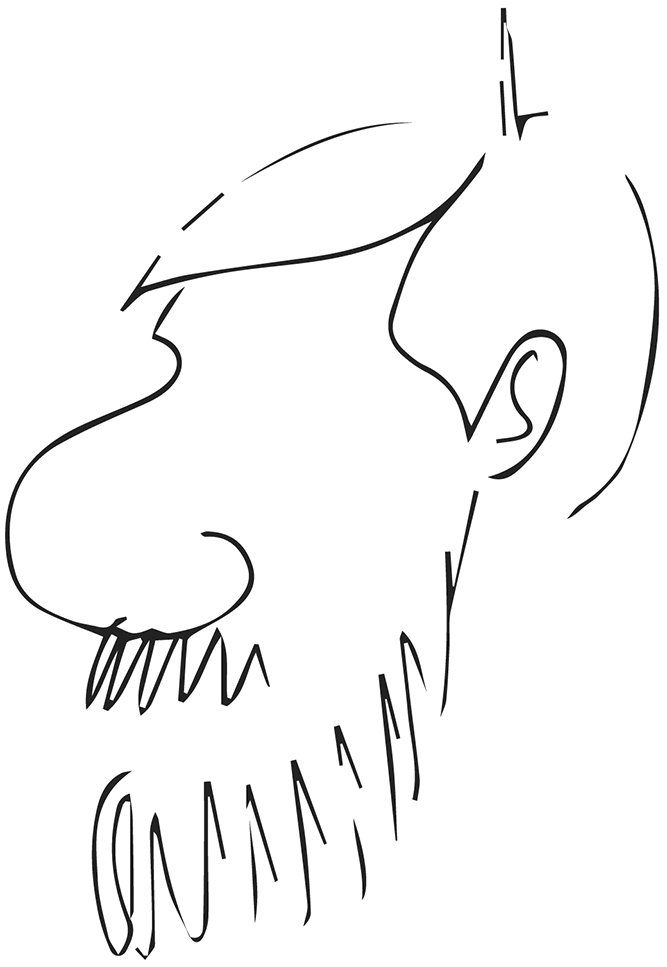
\includegraphics[width=55mm]{./imgs/autocharge.jpg}
%\caption{}
%\end{minipage}
 \end{figure}
\end{vplace}

\clearpage
\thispagestyle{empty}

\movetoevenpage
\pagebreak
\begin{center}
{\MyriadPro{\large\textbf{Posfácio}}}
\end{center}
\label{posfacio}

\bigskip

\emph{O Compromisso} (\emph{Kompromiss,} 1981)\footnote{Traduzido como
  \emph{A troca} no prefácio do livro \emph{Parque Cultural.} Tradução
  Yulia Mikaelyan. São Paulo: Kalinka, 2016.} é mais um capítulo da
epopeia criada pelo escritor russo radicado em Nova Iorque Serguei
Dovlátov (1941--1990) ao longo de seus contos e novelas (seu gênero foi
a prosa curta). Escritas em forma de anedotas tragicômicas, suas obras,
em sua maioria, são conduzidas por um narrador em primeira pessoa
aparentemente muito parecido com seu autor. Como nota o crítico russo
Ígor Sukhikh, vistos em conjunto, seus principais textos --- \emph{A
zona, 1982; O compromisso; O ofício} (\emph{Remesló}),
1985\emph{; Parque Cultural (Zapoviédnik}), 1983; \emph{Os
nossos} (\emph{Náchi}), 1983\emph{, A mala}
(\emph{Tchemodan}), 1986 ---, que espelham as peripécias vividas
ou testemunhadas pelo autor em diferentes momentos de sua vida, são como
que partes integradas de uma única obra, na qual há um único
protagonista: seu autor"-narrador, ou o ``herói lírico
dovlatoviano''.\footnote{\scalebox{0.8}{SUKHIKH}, Ígor. \emph{Serguei Dovlátov: época,
  lugar e destino} (\emph{Serguei Dovlátov:vriemia, miesto, sudbá}). São
  Petersburgo: \emph{Niéstor"-Istória}, 2006, p. 51.}

Nascido em Ufá (Basquíria), durante a Segunda Guerra Mundial, o pequeno
Serioja foi para Leningrado ainda na infância, em 1944. Filho de uma
atriz e revisora armênia e de um diretor teatral judeu, ele desde cedo
teve contato com literatos e, em 1959, ingressou no departamento de
letras finlandesas da Universidade de São Petersburgo, de onde foi
expulso por mau aproveitamento nos estudos. Nessa época, nosso Omar
Sharif (assim alguns amigos chamavam o escritor moreno de quase dois
metros de altura) teve um caso tórrido com uma beldade da cidade, Ássia
Pekuróvskaia, sua primeira esposa. Em 1962, para surpresa de todos, dos
corredores da faculdade e das noitadas literárias regadas a vodca,
Dovlátov foi direto para um \emph{láguer} da República de Kómi, onde
serviu três anos como guarda de prisioneiros escoltados, experiência
explorada em \emph{A zona}.

De volta a Leningrado, o jornalismo tornou"-se seu ganha"-pão, embora,
sobretudo desde o serviço militar, o único ofício ambicionado por ele
fosse o de escritor. Para Dovlátov, ser escritor era a única coisa que
realmente importava, mas, mesmo apreciado por literatos conceituados,
não conseguia ser publicado na União Soviética: parecia estar sempre na
hora errada e no lugar errado. Suas incursões frustradas por diversas
editoras e redações leningradenses são descritas em \emph{O ofício:}
``Tudo o que eu escrevia era aprovado no âmbito dos colaboradores das
revistas ordinárias. Depois, instâncias invi­síveis freavam meus
manuscritos. Eu não chegava a compreen­der quem dirigia a
literatura\ldots{}''.\footnote{\scalebox{0.8}{DOVLÁTOV}, Serguei. \emph{O ofício.} Tradução
  Daniela Mountian e Yulia Mikaelyan. São Paulo: Kalinka, 2017, p. 54.}

Em 1972, brigado com sua segunda mulher, Elena Dovlátova (com quem teve
dois filhos, Ekaterina e, em Nova Iorque, Nikolai) e decepcionado com a
falta de perspectivas profissionais de uma Leningrado conservadora e
burocrática, Serguei Dovlátov saiu em busca de um ambiente criativo
menos asfixiante em Tállin, capital da República Socialista Soviética da
Estônia.

A Estônia, a última república báltica a ser anexada pela União Soviética
(1940), era conhecida por ser um dos lugares menos autoritários do país,
um reduto do liberalismo ocidental, e Tállin por ser uma cidade de
hábitos europeus. Alguns historiadores explicam esse fenômeno como um
vestígio dos vinte e poucos anos de independência estoniana: de 1918,
após a queda do Império Russo, até 1940. Durante a Grande Guerra
Patriótica, a Estônia ainda foi ocupada por tropas nazistas (1941),
voltando ao domínio soviético em 1944 e reconquistando sua independência
em 1991. Anna Koválova e Lev Lurié, autores do livro \emph{Dovlátov,}
descrevem o ambiente da Estônia soviética:

\begin{quote}
Na Estônia, havia mais liberdade do que em qualquer outro lugar do país.
Ali, permitiam as coisas com mais facilidade e as proibiam com menos
prazer. Ali, com boa vontade fechavam os olhos para a apatia política,
não raro ignoravam declarações malvistas, e apenas raramente puniam
erros ideológicos.\footnote{\scalebox{0.8}{KOVÁLOVA}, Anna; \scalebox{0.8}{LURIÉ}, Lev. \emph{Dovlátov}.
  São Petersburgo: \emph{Ámfora}, 2009, p. 176.}
\end{quote}

Não por acaso a cidade estoniana de Tártu deu abrigo ao famoso grupo do
historiador cultural e semioticista Iúri Lótman (1922--1993), este
citado inclusive no \emph{Ofício,} quando uma editora buscava um
parecerista para a publicação do primeiro livro de Dovlátov, \emph{Cinco
esquinas} (\emph{Piat uglóv,} depois renomeado \emph{Contos da cidade,
Gorodskie rasskázy}), coletânea que acabou vetada pelo \scalebox{0.8}{KGB} da
Estônia (o tempo passou: em 2019, o governo de Tállin decidiu erguer uma
estátua em homenagem a Dovlátov, que já possui uma em Petersburgo, além
de uma rua em Nova Iorque com seu nome):

\begin{quote}
Depois de uns dias, ela me telefonou: gostaram muito. Pe­diriam um
parecer de alguém da Universidade de Tállin.

--- Seria possível pedir ao próprio Lótman?

--- Em princípio, sim. Iúri Mikháilovitch escreveria um pa­recer com
prazer. Mas não recomendo. O nome dele despertará um interesse
indesejável. Vamos enviar ao docente Bezzúbov. É muito competente,
especializado na obra de Leonid Andréiev. Gosta de Andréiev? (\scalebox{0.8}{DOVLÁTOV},
2017, p. 71).
\end{quote}

No começo dos anos 1970, escritores soviéticos que não eram aceitos
pelos órgãos oficiais das grandes cidades ainda tinham esperanças de
publicar um livro na pequena República da Estônia. Além da atmosfera
mais liberal, havia poucos escritores contemporâneos russos lá, que,
mesmo sem gozar dos mesmos privilégios dos estonianos, eram valorizados:

\begin{quote}
Com a língua russa, a situação é um pouco diferente. Os au­tores russos
têm possibilidades consideravelmente reduzidas. Embora a sombra tênue
dos privilégios estonianos paire sobre eles também.

Além disso, a seção de literatura russa em Tállin é bem pou­co numerosa.
Fazia três anos que não entravam novos mem­bros na União dos Escritores
local. Por isso se interessaram tanto por mim. (\scalebox{0.8}{DOVLÁTOV}, 2017, p. 72)
\end{quote}

Dessa maneira, Dovlátov considerou a mudança para Tallin uma
possibilidade real de ingressar oficialmente na literatura soviética:
poderia lançar um livro e assim ser admitido na União de Escritores
local. A filiação a uma União de Escritores, mesmo periférica, aumentava
as chances de publicação na União Soviética. Eis os motivos de sua
``primeira emigração'', assim Valéri Popóv\footnote{\scalebox{0.8}{POPÓV}, Valéri.
  \emph{Dovlátov}. Moscou: \emph{Molodaia Gvárdia}, 2010, p. 205.}
definiu a partida do amigo.

Em certo sentido, as expectativas de Dovlátov se concretizaram: em
Tállin, ele logo começou a colaborar num importante jornal da república
editado em russo (a língua oficial do país), o \emph{Estônia Soviética}
(\emph{Soviétskaia Estónia}), tornando"-se um nome respeitado na redação.
A novela \emph{O Compromisso} descreve justamente seu período como
jornalista na imprensa soviética estoniana. O narrador, \emph{alter ego}
do escritor e com quem compartilha o nome, retrata hilariamente o
laboratório de criação de reportagens ``ideologicamente retificadas'' e
muito distantes das situações que as originaram.

\begin{center}
{\MyriadPro{\textbf{Da realidade ao real}}}
\end{center}

Serguei Dovlátov passou dois anos e meio na cidade ``intimista'' de
Tállin, de setembro de 1972 a março de 1975, onde teve oportunidade de
conhecer a fundo as idiossincrasias de uma gazeta soviética. A novela é
composta por 12 partes, ou \emph{compromissos,} que desconstroem a
verdade oficial estampada nas páginas dos jornais. ``Nos jornais
soviéticos só os erros de digitação são fidedignos'', diz um dos
aforismos do escritor que aparece em \emph{Um solo na Underwood},
primeiro volume de seus \emph{Cadernos de anotações}.\footnote{\scalebox{0.8}{DOVLÁTOV},
  Serguei. \emph{Cadernos de anotações. Um solo na Underwood. Um solo no
  \scalebox{0.8}{IBM}} (\emph{Zapisnye kníjki. Solo na Undervude. Solo na \scalebox{0.8}{IBM}}). São
  Petersburgo: \emph{Ázbuka}, 2001, p. 12.}

Os compromissos são iniciados por notícias de jornal (de 1973 a 1976),
seguidas por seus bastidores, ou seja, pela história por trás de cada
uma delas:

\begin{quote}
Não se pode pisar duas vezes no mesmo rio. Mas se pode, através da água,
divisar o fundo coberto por vidros de conservas. E, por trás dos
cenários pomposos do teatro, ver a parede de tijolos, as cordas, o
extintor de incêndio e os operários embriagados. Quem ao menos uma vez
na vida esteve numa coxia sabe disso\ldots{} (\scalebox{0.8}{DOVLÁTOV}, 2019, p.)
\end{quote}

O eixo das anedotas, que mantém a linha narrativa, é a figura do
narrador, o \emph{Serguei Dovlátov ficcional}, o autor das reportagens
que se vê obrigado a assumir o compromisso de conciliar os
acontecimentos hilários, absurdos e às vezes trágicos da realidade que o
cercava com o espaço censurado e ideologicamente alinhado de um jornal
oficial.

O enredo, como geralmente ocorre nos textos de Dovlátov, é baseado em
episódios e pessoas reais. Muitas personagens, antigos colegas e amigos
do escritor, não tiveram nem os nomes modificados: o editor do
\emph{Estônia Soviética} realmente se chamava Guénrikh Frántsevitch
Turónok; Dmítri Kliónski trabalhava no jornal; Ivan Trul era instrutor
do partido. Já na figura de Micha Chablínski é fácil reconhecer o
jornalista Mikhail Roguínski, amigo do escritor desde a faculdade. A
personagem de Marina, a namorada do protagonista, lembra Tamara
Zibunova, engenheira física, com quem Dovlátov morou em Tállin e teve
uma filha, Aleksandra. Érik Buch, por quem suspiravam todas as coroas da
redação, foi baseado no jornalista Mikhail Buch. O jóquei Anatóli
Ivanóv, o ``êmulo do vento'', também teve um protótipo: o jóquei Víktor
Ivanóv, que Dovlátov conheceu ao preparar uma matéria sobre o hipódromo.
É curioso o fato de o jóquei, que quebrou uma perna e duas clavículas ao
cair bêbado de um táxi, ter recebido o nome de um renomado escritor
soviético, Anatóli Stepánovitch Ivanóv (1928 -- 1999). Há quem veja no
hipódromo de Dovlátov uma analogia à distribuição de ordens, títulos e
condecorações aos escritores soviéticos. Aliás, o livro toca em muitos
temas tabus ou em voga, como o alcoolismo, a corrida espacial (no quinto
compromisso há inúmeras referências ao cosmo) e o antissemitismo. Talvez
em nenhum outro livro de Dovlátov a situação dos judeus na União
Soviética tenha sido tão discutida como em \emph{Compromisso}. Por trás
do tom cômico, amoral e despojado do narrador surge um olhar ferino que
não poupa o leitor de verdades desconcertantes:

\begin{quote}
No jornalismo, cada pessoa é autorizada a fazer uma coisa. Violar um
único princípio da moral socialista. Quer dizer, um sujeito pode beber.
Outro ser insolente. Um terceiro contar piadas políticas. Um quarto ser
judeu. Um quinto apartidário. Um sexto levar uma vida imoral. E assim
por diante. Mas cada um, eu repito, só tem permissão para uma coisa. Não
se pode ser judeu e ao mesmo tempo bêbado. Insolente e apartidário\ldots{}
(\scalebox{0.8}{DOVLÁTOV}, 2019, p. \pageref{ref2})
\end{quote}

De forma análoga às personagens, o escritor usou algumas matérias e
reportagens reais como base de seus compromissos. Por exemplo, segundo
colegas do escritor entrevistados por Koválova e Lurié, no jornal
realmente saiu uma carta endereçada a Bréjnev escrita por uma
ordenhadora, porém, a reportagem não fora feita por Dovlátov (que
trabalhava na seção de notícias), mas por um colega da seção de
agricultura (\scalebox{0.8}{KOVÁLOVA}, p. 190). No mesmo livro, Ivan Trul afirmou que no
\emph{Estônia Soviética} existira por algum tempo uma coluna chamada
``Bê"-á"-bá estoniano'', em que eram publicados poemas infantis de
Dovlátov, mas notou que a conversa entre ele e o escritor nunca
acontecera e que a coluna fora fechada por outras razões (\scalebox{0.8}{KOVÁLOVA}, p.
214).

Está claro que o caráter autobiográfico da prosa de Dovlátov é
construído, simulado, são \emph{pseudomemórias}. Sua obra é
essencialmente ficcional, e as pessoas, os acontecimentos e os lugares
servem parar criar o pano de fundo, este sim verdadeiro: as contradições
de viver na União Soviética e da vida em si mesma. Tudo em seus livros,
incluindo o próprio escritor, são peças de seu universo artístico.
Dovlátov manipulava os componentes da realidade que o cercava, misturava
elementos reais e inventados, tornando"-os propositadamente reconhecíveis
para depois desconstruí"-los, contradizê"-los, reafirmá"-los, mitificá"-los.

Mikhail Roguínski, por exemplo, afirma que a mudança de Dovlátov para a
capital estoniana não foi um ato tão espontâneo como descrito na novela
e que o escritor ``chegou a Tállin sozinho e de trem'', e não de carona
com o sinistro Grichánia (\scalebox{0.8}{KOVÁLOVA}, p. 180). Dovlátov não só transforma
a realidade cotidiana como bem entende como dá versões diferentes a um
mesmo episódio, o que não interfere na discussão das grandes questões
(políticas, sociais e mesmo filosóficas) levantadas pela obra. Em
\emph{Ofício} (p. 69), assim ele descreve sua partida de Leningrado:
``Saímos por volta de uma da tarde. Vinte e seis rublos no bolso,
credenciais de jornalista, uma caneta"-tinteiro. Na pasta, uma muda de
roupa de baixo''. Já em \emph{Compromisso} (p. \pageref{ref3}), o
autor"-narrador tinha acabado de sair de uma festa e contava com
dezesseis rublos: ``Demos um pulo numa venda. Garrafas alargavam nossos
bolsos. Eu vestia uma camisa de verão e tênis. Nem sequer carregava o
passaporte''.

Contradições podem também ocorrer numa mesma obra. No oitavo
compromisso, o fotógrafo Jbankóv conta às suas anfitriãs a história da
troca de corpos no enterro de Ilves. No décimo primeiro compromisso, que
descreve o enterro em si, Jbankóv nem aparece, e é Bykovier quem
descobre a trapalhada. Isso poderia ser explicado pelo fato de as
histórias de Dovlátov terem antes sido publicadas separadamente, mas a
decisão de não adaptá"-las, ao reuni"-las, é um ato artístico. Os
``deslizes'' do escritor não são acidentais, mas são usados para
acentuar o caráter ficcional da novela, para criar unidade entre
histórias aparentemente sem ligação, como ainda será visto, ou para
sublinhar uma ideia.

Como não é de admirar, nem todos os conhecidos do escritor gostaram de
ser retratados comicamente em suas obras. O jornalista Dmítri Kliónski,
referindo"-se à personagem que leva seu nome, diz que no livro ``não há
sequer uma palavra de verdade sobre ele'' e que não tinha contato
regular com Serguei Dovlátov, pois, na época, não passava de um
jornalista principiante, enquanto Dovlátov já era um dos ``corifeus'' da
redação (\scalebox{0.8}{KOVÁLOVA}, p. 199). Na mesma entrevista, Kliónski mostrou"-se
indignado com a forma grotesca e irônica em que o editor Turónok fora
descrito, acusando Dovlátov de ingratidão, visto que aquele o apreciava
muito (\scalebox{0.8}{KOVÁLOVA}, p. 202). Não poucos tacharam o escritor de cruel\ldots{} Na
composição de suas personagens, ele podia usar apenas uma característica
de seu modelo, exagerando"-a até torná"-lo uma caricatura. ``Serguei
estava em busca constante por um enredo. Para ele, quase não havia vida
ordinária, tentava imediatamente transpor tudo para o plano de
literatura'', notou Tamara Zibunova (\scalebox{0.8}{KOVÁLOVA}, p. 206).

\begin{center}
{\MyriadPro{\textbf{Dovlátov e a literatura russa}}}
\end{center}

Certamente, a realidade imediata era apenas um pretexto para Serguei
Dovlátov compor suas criações. O tom despretensioso do narrador, como o
de um contador de histórias, pode enganar a um leitor desavisado, mas
figuras literárias memoráveis saíram da pena do escritor. Duas
personagens de \emph{O compromisso} merecem atenção: os impagáveis
Mikhail Jbankóv e Érik Buch.

A personagem do fotógrafo Mikhail Jbankóv, que, pelo visto, não possui
protótipo real, acompanha o autor"-narrador em duas viagens de trabalho:
a primeira para Paide, aonde foram conhecer a vaca recordista, e a
segunda para Tártu, quando foram cobrir o encontro anual de
ex"-prisioneiros de guerra em campos de concentração nazistas. Em seu
desleixo existencial, Jbankóv lembra Mikhal Iványtch ou o fotógrafo
Valera Márkov de \emph{Parque Cultural}, livro em que se descrevem as
agruras do narrador como guia turístico no parque"-museu
Mikháilovskoie"-Trigórskoie, dedicado ao poeta Aleksandr Púchkin, onde
Dovlátov ficou de 1976 a 1977, pouco depois de voltar de Tállin e pouco
antes de emigrar, em 1978 (morando em Nova Iorque desde 1979, finalmente
publicou seus livros, doze ao todo, e tornou"-se um escritor
prestigiado). Jbankóv, representando a figura tragicômica do alcoólatra
russo, é um dos personagens mais lúcidos do enredo. ``E você é feliz?'',
pergunta"-lhe o narrador:

\begin{quote}
\forceindent{}--- Eu? Eu colocaria a corda no pescoço agora mesmo! Tenho medo da dor
do último momento. Se fosse possível adormecer e já não despertar\ldots{}

--- Mas o que fazer?

--- De repente a dor é tão grande que não dá para suportar\ldots{}

--- Mas o que fazer?

--- Não pensar. Beber vodca.

Jbankóv tirou uma garrafa.

--- Parece que vou matar a sede --- disse eu.

--- Como não! --- Jbankóv deu uma piscadela. --- Direto do gargalo?

--- Mas ali tem um copo.

--- O prazer não é o mesmo.

(\scalebox{0.8}{DOVLÁTOV}, 2019, p.)
\end{quote}

Para Jbankóv, a bebida era um meio de escapar à tragicidade da vida.
Essa capacidade do álcool, de harmonizar um mundo de notas dissonantes
(para usar da nomenclatura musical, tão presente no livro), define um
\emph{leitmotiv} da prosa de Dovlátov. Tanto as personagens como o
narrador são consumidos e confortados pela vodca: ``Infelizmente,
revelei grande predisposição para a bebida. Por um tempo, ela me
reconciliava com a realidade'', confessa o autor em \emph{O ofício} (p.
57). O poder sublimador do álcool, ou a passagem etílica para outras
esferas da realidade é um dos motivos que levou alguns críticos a
compararem a obra de Serguei Dovlátov com à de Venedikt Eroféiev
(1938--1991), autor do cultuado ``poema em prosa''
\emph{Moscou"-Petuchki} (1969)\emph{.}

Mas Serguei Dovlátov não deve ser lido apenas ao lado de seus
contemporâneos. Em sua criação existe um profundo diálogo com autores
russos do século 19, dos quais ele apreciava especialmente Anton
Tchékhov, com quem pode ser comparado pelo tom de anedota da primeira
fase tchekhoviana e pela sensação claustrofóbica, de beco sem saída, da
segunda --- sem contar, naturalmente, a concisão e o humor, procedimento
que Dovlátov empregava com precisão cirúrgica. Há inclusive na novela
uma pequena citação ao conto \emph{Enfermaria nº 6}, escrito por
Tchékhov em 1892. No conto, um médico de uma cidadezinha passa a fazer
visitas frequentes a um pavilhão de loucos, atraído pela inteligência de
um dos pacientes, Ivan Dmítrich. A proximidade entre Ivan e o doutor
Andrei Efímitch faz com que este seja declarado insano, sendo no fim
internado na enfermaria nº 6 ao lado de seus consulentes. No quinto
compromisso, Dovlátov se vê às voltas de mais uma incumbência
disparatada de seu editor: para comemorar o Dia da Libertação da
Estônia, precisa ir à maternidade esperar pelo nascimento do
quadringentésimo milésimo habitante da cidade. Após recusar dois bebês,
indesejáveis ao jornal (o primeiro pelo pai vir da Etiópia e a segundo
pelo pai ser judeu), Dovlátov finalmente consegue para sua reportagem
uma criança ``dentro das normas'', cujo pai era um homem alcoólatra e
frustrado, mas russo:

\begin{quote}
--- Kúzina, da enfermaria nº 6, deu à luz. Aqui estão os dados. Ela é
estoniana, motorista de carrinhos de carga. O marido, um torneiro da
fábrica de navios, é russo, membro do partido. O bebê está dentro das
normas. (\scalebox{0.8}{DOVLÁTOV}, 2019, p. \pageref{ref4})
\end{quote}

Outro louco lúcido do enredo é Érik Buch, um belo jornalista de trinta e
poucos anos, cobiçado pelas mulheres de meia"-idade do jornal, que parece
ter nascido em outra época. De acordo com Roguínski, Mikhail Buch, o
modelo de Érik, era de fato mulherengo, vivia em apuros na redação e não
conseguia emprego fixo, pois era descuidado ao checar as fontes de suas
matérias (como se deu com a entrevista do capitão de um navio mercante
alemão, Paul Rudi, na verdade um estoniano foragido), mas a personagem
do jornalista tem outras camadas de significado. Como um Quixote
soviético, a figura ambivalente de Buch (``Nele a insubmissão convivia
pacificamente com a ausência de princípios'') tem uma espécie de
nobreza, na sua luta solitária contra as arbitrariedades do mundo e na
relação com Dovlátov:

\begin{quote}
Buch refletiu um segundo, como se estivesse tomando uma decisão difícil.

--- Quer casar com Galina? --- disse ele. --- Eu cedo Galina a você, meu
amigo. Ela pode pintar flores para vender. E daqui a uma semana vai
nascer uma ninhada de siameses. Case, não vai se arrepender! (\scalebox{0.8}{DOVLÁTOV},
2019, p. \pageref{ref5})
\end{quote}

Érik Buch, assim como Jbankóv, não deixa de ser uma atualização do
\emph{homem pequeno} (\emph{málenkii tcheloviek}), tipo consagrado na
literatura russa por personagens como Akáki Akákievitch (\emph{O
capote,} Gógol, 1842), um funcionário insignificante de uma
repartição que tem um ímpeto de vida quando se vê obrigado a encomendar
um novo capote e, depois de morto, passa a assombrar os habitantes de
São Petersburgo. Essas vidas ordinárias, anônimas e decaídas povoaram as
páginas da literatura russa do século 19, perdendo espaço durante o
realismo socialista, mas o reconquistando nos anos 1960 e 1970, quando
escritores não oficiais se voltaram para esferas marginalizadas da
sociedade soviética (como também o fez, por exemplo, Liudmila
Petruchévskaia, já conhecida do público brasileiro). Após desperdiçar
sua última chance de ter um cargo efetivo no jornal, Buch sai vagando,
ébrio e degradado, pelas ruas estonianas, tornando"-se um ponto
indefinido no espaço. Em sua indolência e delírio (``(\ldots{}) passava dias
inteiros metido num penhoar verde que Galina havia costurado da cortina
da janela. Ele preparava o discurso que pronunciaria ao ser agraciado
com o Nobel (\ldots{})''), Buch também tem um quê de Oblómov, de um
\emph{homem supérfluo} (\emph{líchnii tcheloviék}), que, em desacordo
com a realidade e pleno de ideais, é incapaz de realizar"-se.

Referindo"-se a alguns personagens de Dovlátov, Ígor Sukhikh (2006, p.
109) propõe inverter a fórmula gogoliana do ``riso entre lágrimas''. De
fato, no caso de Jbankóv e de Buch, em alguns momentos brotam ``lágrimas
entre risos''. Revela"-se o dom de Dovlátov de unir o cômico e o
dramático, o triste e o alegre, o patético e o genial. Assim como o Ivan
da \emph{Enfermaria nº 6}, Jbankóv e Buch eram homens de talento:
Jbankóv, munido de uma antiga máquina soviética de nove rublos, era um
excelente fotógrafo e Buch destacava"-se visivelmente em meio à
mediocridade dos jornalistas locais.

Em todo caso, a citação mais flagrante do enredo certamente envolve
Fiódor Dostoiévski. Como notou Galina Dobrozrákova,\footnote{\scalebox{0.8}{DOBROZRÁKOVA},
  Galina. \emph{Dostoiévski na consciência artística de S. Dovlátov}
  (\emph{Dostoiévski v khudójestvennom soznánii S. Dovlátova})\emph{.
  Viéstnik Sam\scalebox{0.8}{GU},} nº4 (85), 2011.} no décimo primeiro
compromisso, em que são narrados os quiproquós ocorridos durante o
enterro de Hubert Ilves, o diretor do estúdio de televisão, foi
delineado um claro diálogo paródico com \emph{Bobók}, que Dovlátov
considerava o melhor conto de todos os tempos, por nele sobressair a
``natureza ambivalente do riso de Dostoiévski''(\scalebox{0.8}{DOBROZRÁKOVA}, p. 1). No
gogoliano \emph{Bobók,} lançado em 1873 na coluna \emph{Diário de um
escritor} (revista \emph{O cidadão}), um escrevinhador escuta
vozes do além num cemitério, vozes das procedências mais distintas que,
igualadas na morte, têm o mesmo direito de existir\emph{. }

Mesmo antes de o narrador de \emph{O compromisso} ouvir uma ``voz
distante'', vinda de dentro da sepultura --- ``No que estou pensando, do
lado de cá da cova? Nos mistérios da alma humana. Na superação da morte
e dos pesares do espírito. Nas leis da existência que nasceram há
milênios e que continuarão vivas até o sol deixar de brilhar\ldots{}'' (p. \pageref{ref6})
---, a narrativa vai demarcando aproximações com o pequeno conto
fantástico de Dostoiévski (\scalebox{0.8}{DOBROZRÁKOVA}, p. 3). Em \emph{Bobók,} o
narrador em primeira pessoa, também um bêbado russo (``Ivan Ivánovitch,
diz, por favor, vou encontrar"-te sóbrio algum dia?'')\footnote{\scalebox{0.8}{DOSTOIÉVSKI},
  Fiódor. \emph{Bobók} \&\emph{Meia carta ``de um sujeito''.} Tradução
  Daniela e Moissei Mountian. Coleção Mir. São Paulo: Kalinka, 2018, p.
  9.} e também um literato frustrado (``Escrevi uma novela ---
recusaram. Escrevi um folhetim --- recusaram''), vai a um enterro de um
parente distante, mas um ``conselheiro do colegiado''. Depois de passar
por um restaurante e de tomar uns goles, senta ao lado de uma lápide e
vê um sanduíche largado: ``fato estúpido e inoportuno''. Já os três
incorrigíveis amigos, Dovlátov, Bykovier e Altmäe, unidos pela vodca,
levam o defunto de Ilves para o cemitério espremidos num furgão de
metal, onde bebem e comem sanduíches, colocados sobre a tampa do caixão.
No cemitério de \emph{Bobók}, o narrador se queixa do peso do defunto:

\begin{quote}
Depois, ajudei, com minhas próprias mãos, a carregar o caixão da igreja
até a sepultura. Por que será que os mortos no caixão ficam tão pesados?
Dizem que, devido a algum tipo de inércia, é como se o corpo já não se
controlasse sozinho\ldots{} ou qualquer outro absurdo do gênero, o que
contradiz a mecânica e o bom senso. (\scalebox{0.8}{DOSTOIÉVSKI}, 2018, p. 21)
\end{quote}

Em \emph{Compromisso,} Fima Bykovier, judeu semilouco e genial, por
pouco não deixa o caixão cair: ``Como é pesado, parasita\ldots{}''. Ao andar
pelo cemitério, Ivan Ivánovitch espia dentro das sepulturas e ``havia
água lá, e que espécie de água!''. Dovlátov, aproximando"-se da cova para
fazer o discurso de que fora encarregado, menciona: ``Ali dentro havia
água parada (\ldots{}).''

Falar de \emph{Bobók} é quase sinônimo de falar de Mikhail Bakhtin
(1895--1975), crítico que consagrou\footnote{\scalebox{0.8}{BAKHTIN}, Mikhail.
  \emph{Problemas da poética de Dostoiévski.} Tradução Paulo Bezerra.
  Rio de Janeiro: Forense Universitária, 2005.} o conto como um modelo
da sátira menipeia, estilo que, segundo ele, teria dado origem à
literatura carnavalizada, à qual Dostoiévski estaria filiado, culminando
em sua tão discutida polifonia, ou a ``multiplicidade de consciências,
plenamente qualificadas, cada uma com seu mundo e seu pensamento por
trás''.\footnote{\scalebox{0.8}{BERNARDINI}, Aurora Fornoni. \emph{Aulas de literatura
  russa: de Púchkin a Gorenstein.} São Paulo: Kalinka, 2018, p. 124.}

Na relação entre Dovlátov e \emph{Bobók,} Galina Dobrozrákova (p. 2) vai
mais longe: considera bem provável que Dovlátov, atento a críticos e
estudos literários, tivesse contato com essa interpretação de Bakhtin, e
que ambos, a obra e seu interpretador, tenham servido de fonte para a
composição da novela.

Sem entrar em detalhes, lembremos apenas que na carnavalização (a
transposição da festa para a literatura) descrita por Bakhtin reina a
temporalidade do extraordinário, de um estado de exceção, cheio do
grotesco e da bufonaria. Aqui os gêneros, os tons e os estilos podem
conviver sem barreiras, todas as regras e as leis habituais perdem
validade, e todas as vozes têm expressão livre: ``O carnaval aproxima,
reúne, celebra os esponsais e combina o sagrado com o profano, o elevado
com o baixo, o grande com o insignificante, etc.'' (\scalebox{0.8}{BAKHTIN}, 2005, p.
123). Nesse mundo de ponta"-cabeça, elimina"-se a distância entre os
homens, anulam"-se as hierarquias, invertem"-se os papéis, reúnem"-se o
riso e a morte.

Essa ambivalência está presente no andar rocambolesco do enterro de
Ilves, em que o profano e o sagrado são continuamente misturados, e a
paródia fica demarcada no fim: enquanto, em \emph{Bobók,} Ivan
Ivánovitch escuta risos e zombarias dos mortos, Dovlátov ouve um
discurso lúcido e triste, mas ambos fazem, via riso e via fantástico,
com o que o leitor experimente uma verdade, usando de um conceito de
Bakhtin, como nota também Galina Dobrozrákova (p. 4).

Se existe nesse episódio da novela uma conversa particular com
\emph{Bobók,} há um elemento carnavalesco que transpassa todos os
\emph{compromissos} e basicamente todos os livros de Dovlátov: a
sensação de caos, de uma situação em crise, de um mundo virado às
avessas, como, inclusive, na \emph{Enfermaria nº 6}. ``Porque o pior não
é o pesadelo e a sensação de beco sem saída. O mais terrível é o
caos\ldots{}'', diz Alikhánov, o narrador de \emph{Parque Cultural} (p. 87).
Paulo Bezerra, em ensaio sobre \emph{Bobók,} escreve sobre a sátira
menipeia:

\begin{quote}
O caos que toma conta do mundo representa um questionamento do
\emph{status quo}, o presente está em processo de formação e o passado
não serve mais como modelo. O riso aproxima e dá o tom a tudo, sua
ambivalência vislumbra uma nova perspectiva de construção do universo,
assumindo, em casos particulares, conotações utópicas. O riso
familiariza tudo e não deixa mais lugar para a imagem elevada do passado
absoluto, todo o espaço da representação se constitui numa zona de
contato familiar entre o mais sagrado e o mais profano, o mais alto e o
mais baixo (\ldots{})\footnote{\scalebox{0.8}{DOSTOIÉVSKI}, Fiódor. \emph{Dostoiévski:
  ``Bobók''.} Tradução e análise do conto Paulo Bezerra. São Paulo:
  Editora 34, p. 110.}
\end{quote}

Por trás da narração descontraída de Dovlátov, do tom cômico,
confessional e amigo que não se presta a dar sermões, surge um autor em
busca por harmonia. Numa entrevista dada a John Glad, Dovlátov discorre
sobre o caos, que, enquanto cosmovisão, é um elemento inseparável da
literatura russa:

\begin{quote}
Eu tento despertar no leitor a sensação de normalidade\ldots{} Um dos
sentimentos mais sérios ligados ao nosso tempo é a sensação do absurdo
iminente, quando a loucura se converte num fenômeno mais ou menos
normal\ldots{} Isso significa que o absurdo e a loucura se transformam em
algo completamente natural, e a norma, quer dizer, uma conduta normal,
natural, generosa, tranquila, discreta, educada se torna, cada vez mais,
um acontecimento fora do comum\ldots{} Despertar no leitor a sensação de que
isso é normal, talvez eu não me coloque de caso pensado diante dessa
tarefa, mas é o meu tema, um tema que eu não inventei e ao qual não sou
o único a dedicar algum tempo e esforço. Se palavras bonitas e, em
geral, corretas e justas são necessárias, isso é uma tentativa de
harmonização do mundo.\footnote{\scalebox{0.8}{SUKHIKH}, Ígor. \emph{Literatura russa
  para todos} (\emph{Rússkaia literatura dlia vsekh}), tomo 3.
  Petersburgo: Lenizdat, 2013, p. 696.}
\end{quote}

Em 2015, durante a abertura do Festival Serguei Dovlátov (Pskóv), o
crítico e escritor russo Víktor Eroféiev destaca essa natureza
harmonizadora, cheia de humor e ironia, numa entrevista sobre o
homenageado (Dovlátov teve um infarto fulminante antes dos 50 anos, em
Nova Iorque, quando começava a se tornar conhecido na Rússia e, desde
então, quase trinta anos após sua morte, vem ganhando admiradores):

\begin{quote}
As pessoas precisam de uma referência moral da época em que vivemos. É
difícil encontrar isso, e nesse ponto Dovlátov ajuda muito\ldots{} Dovlátov
achou para si uma posição muito equilibrada: um observador um tanto
cruel e, ao mesmo tempo, irônico e espirituoso. Como Tchékhov, ele tinha
a capacidade magnífica de misturar o importante e o insignificante
(\ldots{}).\footnote{Entrevista disponível em \textless{}
  \emph{https://bit.ly/2EzGxlj}\textgreater{}.}
\end{quote}

\begin{center}
{\MyriadPro{\textbf{Dovlátov \emph{versus} Dovlátov}}}
\end{center}

Ainda no enterro de Ilves, no décimo primeiro compromisso, Galina
Dobrozrákova (pág. 3) chama a atenção para outro componente da
carnavalização: a troca incessante de papéis, a inversão de valores.
Dovlátov foi ao enterro no lugar de Chablínski e vestido com um terno do
colega (e também o substituiu na relação com Marina); Bykovier fora
mandado a um \emph{láguer} por sua voz ter sido confundida com a de
Stálin; e, a apoteose, o corpo de Ilves foi trocado pelo de um contador
do \emph{kolkhoz} de pescadores: o alto funcionário foi enterrado num
cemitério como um homem comum e o simples contador recebeu as honras de
um homem da nomenclatura, num cemitério apenas para privilegiados. Essa
troca de papéis, além de ser o mote da novela (notícias que não são o
que aparentam ser), é aplicada --- com detalhes que o leitor se
divertirá ao descobrir --- em outros momentos do enredo, delineando uma
espécie de unidade entre as histórias, unidade salientada ainda por
elementos ou cenas recorrentes, como, por exemplo, o uso do algarismo 4
(o quadringentésimo milésimo habitante da cidade nasceu no hospital nº
4; a cientista em busca de conselhos sobre sexo corria a prova dos 400
metros; o telefone de Buch era 4-0-0-11; Jbankóv usava o filme
\emph{Mikrat nº4;} etc.) No entanto, talvez a utilização mais
interessante da alternância de papéis, do mascaramento, da produção de
\emph{duplos,} seja a do narrador, que muda de lugar consigo próprio (o
que o autor inclusive aplica em outras obras).

A paródia carnavalesca está inevitavelmente embebida do elemento cômico,
mas ele não é usado apenas para negar e deformar, mas para renovar. Um
desdobramento dessa ideia seria a criação de personagens que são negadas
e afirmadas por outras, pelos seus duplos. Essa característica é notada
por Bakhtin no conjunto da obra de Dostoiévski --- Raskólnikov, por
exemplo, é negado e reiterado por Svidrigáilov, Lújin, Stravóguin, Ivan
Karamázov e até pelo diabo. São personagens que se desdobram em si
mesmas por meio de um processo de construção complementar ambivalente. É
como se Raskólnikov morresse em cada uma delas para afirmar sua
presença, num estranho jogo de espelhos.

No sexto compromisso, Lida Agápova, procurando uma ``pessoa
interessante'' para entrevistar em seu programa de rádio, lembrou"-se de
Alikhánov:

\begin{quote}
Outro dia uma colega jornalista havia aparecido na rádio com um
filólogo\ldots{} Ou talvez fosse tradutor. Ele disse que tinha sido guarda de
prisioneiros escoltados\ldots{} Contava coisas horríveis\ldots{} O sobrenome dele
não era russo, Alikhánov. Outra pessoa interessante, sem sombra de
dúvida\ldots{} (\scalebox{0.8}{DOVLÁTOV}, 2019, p. \pageref{ref1})
\end{quote}

Boris Alikhánov é o autor"-narrador de duas novelas, \emph{Parque
Cultural} e \emph{A zona}, mas é sobretudo a segunda que é aqui
recuperada (o escritor às vezes dava seu próprio nome aos narradores, às
vezes não, mas todos são propositadamente aproximados de sua figura
real, inclusive fisicamente). Se Dovlátov é por vezes considerado
impiedoso pela forma em que transformou seus amigos em personagens, nada
se compara com o tratamento que ele podia dar ao seu eu ficcional. Em
\emph{O compromisso} ele fez uma caricatura cruel de Alikhánov: a
personagem, de testa pequena, queixo frouxo e um ``quê de falso
napolitano no olhar'' (o escritor costumava se descrever assim), era
alcoólatra, vivia na imundície, mal conseguia terminar uma frase
(``desmanchou"-se num discurso inábil e sem sentido que não pôde
acabar'') e estava tão emocionalmente exaurido que destruiu todos os
méritos de sua experiência num \emph{láguer}:

\begin{quote}
\forceindent{}--- Liuba --- disse ele.

--- Lida.

--- Lida! --- Alikhánov quase gritava. --- Vou pegar agora seis rublos.
Tenho vizinhos humanos. Vamos comprar meia garrafa de vodca e uma de
vinho seco. Não estou concatenando as ideias.

--- Não bebo. O senhor se considera um homem corajoso?

--- Não sei. Antes eu conseguia tomar dois litros. Agora bastam
setecentos gramas para eu ficar tonto\ldots{} É a idade\ldots{}

(\scalebox{0.8}{DOVLÁTOV}, 2019, p. \pageref{ref7})
\end{quote}

Mesmo a cicatriz de Alikhánov --- referência à novela \emph{A zona,} em
que ficamos sabendo que o narrador foi ferido por um dos presos --- aqui
foi transformada num furúnculo. Mas a ideia principal de \emph{A zona}
não se perde: as fronteiras pouco claras entre os guardas e os
prisioneiros, entre a prisão e a liberdade:

\begin{quote}
\forceindent{}--- O senhor não compreendeu. Preciso de um homem original, de uma
personalidade interessante. O senhor é filólogo, um indivíduo que sente
as coisas com delicadeza. E antes era um guarda num campo de
prisioneiros. Corria riscos todo santo dia. A delicadeza da alma
frequentemente vem acompanhada pela rudeza física.

--- Quando é que eu fui rude com a senhora?

--- Não comigo. O senhor vigiava os presos\ldots{}

--- Vigiávamos principalmente a nós mesmos. 

(\scalebox{0.8}{DOVLÁTOV}, 2019, p. \pageref{ref8})
\end{quote}

De volta ao décimo primeiro compromisso, enquanto levava o corpo de
Ilves para o cemitério, o narrador, Serguei Dovlátov, recorda"-se de seu
tempo de guarda de um campo de prisioneiros, trocando de lugar consigo
próprio outra vez, e, para completar, antes de seu discurso, ele é
apresentado como Dolmátov, nome do narrador da novela \emph{Filial}
(1987):

\begin{quote}
\forceindent{}--- As palavras de despedida são de\ldots{}

Claro que ele mutilou meu sobrenome:

--- As palavras de despedida são do camarada Dolmátov.

Quantos homens já não fui nesta vida? Dokládov, Zaplátov\ldots{}

(\scalebox{0.8}{DOVLÁTOV}, 2019, p. \pageref{ref9})
\end{quote}

Com o duplo do duplo, o sósia do sósia, o narrador Serguei Dovlátov,
também relacionado com o autor, também relacionado com o escritor, morre
dostoievskianamente em si mesmo e nos mostra que a coisa mais verdadeira
do livro é sua arte.

\begin{flushright}
\emph{Daniela Mountian e Yulia Mikaelyan}
\end{flushright}
